% \documentclass[anon,12pt]{colt2018} % Anonymized submission
\documentclass[12pt]{colt2018} % Include author names
% http://www.learningtheory.org/colt2018/call.html#instructions

% The following packages will be automatically loaded:
% amsmath, amssymb, natbib, graphicx, url, algorithm2e

\title[What Doubling Tricks Can and Cannot Do for Multi-Armed Bandits]{What Doubling Tricks Can and Cannot Do for Multi-Armed Bandits}

\usepackage{macrosArticle}
\usepackage{macrosText}
\usepackage{times}
\usepackage{array}
\usepackage{float}

\coltauthor{\Name{Lilian Besson} \Email{{Lilian}{.}{Besson}{@}{CentraleSupelec}{.}{fr}} \\
    \addr CentraleSup\'elec (campus of Rennes), IETR, SCEE Team,\\
    Avenue de la Boulaie -- CS $47601$, F-$35576$ Cesson-S\'evign\'e, France
    \AND
    \Name{Emilie Kaufmann} \Email{{Emilie}{.}{Kaufmann}{@}{Univ}{-}{Lille}{.}{fr}} \\
    \addr CNRS \& Universit\'e de Lille, Inria SequeL team\\
    UMR $9189$ -- CRIStAL,  F-$59000$ Lille, France
}

\begin{document}

\maketitle


% -----------------------------------------------------------------
\begin{abstract}
    An online reinforcement learning algorithm is \emph{anytime} if it does not need to know in advance the horizon $T$ of the experiment.
    A well-known technique to obtain an anytime algorithm from any non-anytime algorithm is the ``Doubling Trick''.
    In the context of adversarial or stochastic multi-armed bandits,
    the performance of an algorithm is measured by its regret,
    and we study two families of sequences of growing horizons (geometric and exponential)
    to generalize previously known results that certain doubling tricks can be used to conserve certain regret bounds.
    In a broad setting, we prove that a geometric doubling trick can be used to conserve (minimax) bounds in $R_T = \cO(\sqrt{T})$ but \emph{cannot} conserve (distribution-dependent) bounds in $R_T = \cO(\log T)$.
    We give insights as to why exponential doubling tricks may be better, as they conserve bounds in $R_T = \cO(\log T)$, and are close to conserving bounds in $R_T = \cO(\sqrt{T})$.
    %
    % Numerical experiments also show the efficiency of this approach
    % when the appropriate doubling trick is used with
    % efficient non-anytime algorithms,
    % like the Approximated Finite-Horizons Gittins Index (\AFHG) algorithm by \cite{Lattimore16a} or \KLUCBpp{} by \cite{Menard17}.

    % DEADLINE
    % - Paper submission deadline: February 16, 2018, 11:00 PM EST
    % \verb+http://www.learningtheory.org/colt2018/call.html#instructions+
\end{abstract}

% -----------------------------------------------------------------
\begin{keywords}
    Multi-Armed Bandits;
    % Reinforcement Learning;
    % Online Learning;
    Anytime Algorithms;
    Sequential Learning;
    Doubling Trick.
\end{keywords}


% \iffalse  % XXX
\FIXME{
    Remove Table of Contents when submitting.
    Maybe bring back table of content for the HAL version?
}
\tableofcontents
% \fi % XXX


\TODO{Maths:}
\begin{enumerate}
    % \item Write a code that plots, for a function $f$,
    % \[\frac{\sum_{i=0}^{L_T} (T_i - T_{i-1})^{\gamma} \log(T_i - T_{i-1})^{\delta}}{T^{\gamma} (\log(T))^{\delta}}\]
    % (and the same without the $T_{i-1}$), just to have an idea how bad is our initial upper bound
    \item Is a function for which it is bounded for $(\gamma,\delta)=(1/2,0)$ and $(\gamma,\delta)=(0,1)$ then prove it mathematically!
    \item Extend the lower bound at the end of this document for all $\alpha \in (0,1]$
    \item Include also the previous geometric lower bound in this statement
\end{enumerate}

\TODO{Writing:}
\begin{itemize}
    \item Change introduction,
\end{itemize}
% -----------------------------------------------------------------


% -----------------------------------------------------------------
\section{Introduction}
% -----------------------------------------------------------------

\todo[inline]{begin todo}
    \begin{itemize}
        \item
        Change the motivation:
        understanding why those doubling tricks are used, and what they can preserve...
        \item
        Remove the idea of problem dependent + worse-case optimal
        \item
        Update the literature review:
        Talk about the \KLUCBswitch{} algorithm from \cite{GarivierHadiji2018}.
    \end{itemize}
\todo[inline]{end todo}

Multi-Armed Bandit (MAB) problems are well-studied sequential decision making problems in which an agent repeatedly chooses an action (the ``arm'' of a one-armed bandit) in order to maximize some total reward \citep{Robbins52,LaiRobbins85}.
Initial motivation for their study came from the modeling of clinical trials, as early as 1933 with the seminal work of \cite{Thompson33}.
In this example, arms correspond to different treatments with unknown, random effect.
Since then, MAB models have been proved useful for many more applications, that range from
cognitive radio \citep{Jouini09} to
online content optimization (\eg, news article recommendation \citep{Li10}, online advertising \citep{LiChapelle11}, A/B Testing \citep{Kaufmann14,Jamieson17ABTest}),
or portfolio optimization \citep{Sani2012risk}.

While the number of patients involved in a clinical study (and thus the number of treatments to select) is often decided in advance, in other contexts the total number of decisions to make (the horizon $T$) is unknown.
It may correspond to the total number of visitors of a website optimizing its displays for a certain period of time, or to the number of attempted communications in a smart radio device.
In such cases, it is thus crucial to devise \emph{anytime algorithms}, that is algorithms that do no rely on the knowledge of this horizon $T$ to sequentially select arms.
A general way to turn any base algorithm into an anytime algorithm is the use of the so-called Doubling Trick, first proposed by \cite{auer1995gambling}, that consists in repeatedly running the base algorithm with increasing horizons.
Motivated by the frequent use of this technique and the absence of a generic study of its effect on the algorithm's efficiency,
this paper investigates in details two families of doubling sequences (geometric and exponential), and shows that the former should be avoided for stochastic problems.


More formally, a MAB model is a set of $K$ arms, each arm $k$ being associated to a (unknown) \emph{reward stream} $(Y_{k,t})_{t\in\N}$.
Fix $T$ a finite (possibly unknown) horizon.
At each time step $t \in \{1,\dots,T\}$ an agent selects an arm $A(t) \in \{1,\dots,K\}$ and receives as a reward the current value of the associated reward stream, $r(t) := Y_{A(t), t}$.
The agent's decision strategy (or \emph{bandit algorithm})
$\cA_T := (A(t), t\in \{1,\dots,T\})$ is such that $A(t)$ can only rely on the past observations
% $\cF_{t-1} = (A(1),r(1),\dots,A(t-1),r(t-1))$,
$A(1),r(1),\dots,A(t-1),r(t-1)$,
on external randomness and (possibly) on the knowledge of the horizon $T$.
The objective of the agent is to find an algorithm $\cA$ that maximizes the expected cumulated rewards, where the expectation is taken over the possible randomness used by the algorithm and the possible randomness in the generation of the rewards stream.
In the oblivious case, in which the reward streams are independent of the algorithm's choice, this is equivalent to minimizing the \emph{regret}, defined as
\begin{equation}\label{eq:regret}
    R_T(\cA_T) := \max_{k \in \{1,\dots,K\}}
    % \mu^* T - \E_{\mu}\left[\sum_{t=1}^{T} r(t)\right]
    \E\left[\sum_{t=1}^{T} \left(Y_{k,t} - Y_{A(t),t}\right)\right].
    % = \mu^* T - \sum_{k=1}^K \mu_k \E_{\mu}\left[ T_k(T) \right], \
\end{equation}


This quantity, referred to as \emph{pseudo-regret} in \cite{Bubeck12}, quantifies the difference between the expected cumulated reward of the best fixed action, and that of the strategy $\cA_T$.
For the general adversarial bandit problem \citep{Auer02NonStochastic}, in which the rewards streams are arbitrary (picked by an adversary), a \emph{worst-case} lower bound has been given.
It says that for every algorithm, there exists (stochastic) reward streams such that the regret is larger than $(1/20)\sqrt{KT}$
\citep{Auer02NonStochastic}.
% \citep[Th.5.1]{Auer02NonStochastic}.
Besides, the \ExpThree{} algorithm has been shown to have a regret of order $\sqrt{KT\log(K)}$.


Much smaller regret may be obtained in \emph{stochastic} MAB models, in which the reward stream from each arm $k$ is assumed to be \iid, from some (unknown) distribution $\nu_k$, with mean $\mu_k$.
In that case, various algorithms have been proposed with \emph{problem-dependent} regret upper bounds of the form $C(\bm\nu) \log(T),$ where $C(\bm\nu)$ is a constant that only depend on the arms distributions.
Different assumptions on the arms distributions lead to different problem-dependent constants.
In particular, under some parametric assumptions (\eg, Gaussian distributions, exponential families), \emph{asymptotically optimal} algorithms have been proposed and analyzed (\eg, \KLUCB{} \citep{KLUCBJournal} or Thompson sampling \citep{AgrawalGoyal11,Kaufmann12Thompson}), for which the constant $C(\bm\nu)$ obtained in the regret upper bound matches exactly that of the lower bound given by \cite{LaiRobbins85}.
Under the non-parametric assumption that the $\nu_k$ are bounded in $[0,1]$, the regret of the \UCBone{} algorithm \citep{Auer02} is of the above form with $C(\bm\nu) = 8 \times \sum_{k : \mu_k > \mu^*} (\mu^* - \mu_k)^{-1}$, where $\mu^* = \max_k \mu_k$ is the mean of the best arm.
%\UCBone{} is referred to as \emph{order-optimal} as its regret has, up to a multiplicative constant, the right dependency in the gaps.
Like in this last example, all the available constants $C(\bm\nu)$ become very large on ``hard'' instances, in which some arms are very close to the best arm.
On such instances,  $C(\bm\nu)\log(T)$ may be much larger than the worst-case $(1/20)\sqrt{KT}$, and distribution-independent guarantees may actually be preferred.

The \MOSS{} algorithm, proposed by \cite{Audibert2009minimax}, is the first stochastic bandit algorithm
to enjoy a problem-dependent logarithmic regret
and to be optimal in a \emph{minimax} sense, as its regret is proved to be upper bounded by $\sqrt{KT}$, for bandit models with rewards in $[0,1]$.
However the corresponding constant $C(\bm \nu)$ is proportional to $K/\Delta_{\min}$, where $\Delta_{\min} = \min_{k} (\mu^*-\mu_k)$ is the minimal gap, which worsen the constant of \UCBone{}.
Another drawback of \MOSS{} is that it is \emph{not} anytime.
%
These two shortcoming have been overcame recently in two different works.
On the one hand, the \MOSSAnytime{} algorithm \citep{Degenne16} is minimax optimal and anytime, but its problem-dependent regret does not improve that of \MOSS.
On the other hand, the \KLUCBpp{} algorithm \citep{Menard17} is simultaneously minimax optimal and asymptotically optimal (\ie, it has the best problem-dependent constant $C(\bm\nu)$), but it is not anytime. A natural question is thus to know whether a Doubling Trick could overcome this limitation.


This question is the starting point of our comprehensive study of the Doubling Trick: can a single Doubling Trick be used to preserve both problem-dependent (logarithmic) regret and minimax (square-root) regret?
We answer this question partially, by showing that two different types of Doubling Trick may actually be needed.
In this paper, we investigate how algorithms enjoying regret guarantees of the generic form
\begin{equation}\label{eq:genericWithLogT}
    \forall T \geq 1,\;\;\;\; R_T(\cA_T) \leq c \; T^{\gamma} (\log T)^{\delta} + o( T^{\gamma} \left(\log T)^{\delta} \right)
\end{equation}
may be turned into an anytime algorithm enjoying \emph{similar} regret guarantees with an appropriate Doubling Trick.
%
This does not come for free, and we exhibit a ``price of Doubling Trick'', that is a constant factor larger than $1$, referred to as a \emph{constant multiplicative overhead}.



% Outline of this article
%\paragraph{Outline}
The rest of the paper is organized as follows.
The Doubling Trick is formally defined in Section~\ref{sec:genericAlgo}, along with a generic tool for its analysis.
In Section~\ref{sec:geometricDoublingTrick}, we present upper and lower bounds on the regret of algorithms to which a geometric Doubling Trick is applied.
Section~\ref{sec:exponentialDoublingTrick} investigates regret guarantees that can be obtained for a ``faster'' exponential Doubling Trick.
Experimental results are then reported in Section~\ref{sec:experiments}.
Complementary elements of proofs are deferred to the appendix.
% We give missing proofs and additional results in Appendix~\ref{sec:missingproofs}, a heuristic $\DTnr$ improving $\DTr$ in App.~\ref{sec:DTnr} along with more experimental results in App.~\ref{sec:otherExperiments}, and other technical tools are given in App.~\ref{sec:otherproofs}.

% -----------------------------------------------------------------
\section{Doubling Tricks }\label{sec:genericAlgo}


The Doubling Trick, denoted by \DT, is a general procedure to convert a (possibly non-anytime) algorithm into an anytime algorithm.
It is formally stated below as Algorithm~\ref{algo:DTr} and depends on a non-decreasing diverging \emph{doubling sequence} $(T_i)_{i\in \N}$
(\ie, $T_i\to\infty$ for $i\to\infty$).
% such that $T_i$ goes to infinity.
\DT{} fully restarts the underlying algorithm $\cA$ at the beginning of each new sequence (at $t = T_i + 1$), and run this algorithm on a sequence of length ($T_i - T_{i-1}$).
% If the algorithm $\cA$ needs to know the horizon, $\cA_{T=\square}$ denotes $\cA$ initialized with the value $\square$ for its parameter $T$,
% and if $\cA$ does not need the horizon, $\cA_{T=\square}$ is simply a new instance of $\cA$.

% \FIXME{Remove box ?}

%
%It is immediate to check that for any $t$, the decisions taken by $\cA' = \DTr(\cA, (T_i)_{i\in\N})$, $A'(t)$, are also measurable regarding the previous observations.

%
%It is a very generic\footnote{It is well known to not even be restricted to the setting of Multi-Armed Bandit.} algorithm that can be applied to any algorithm $A$.
%

% - Full restart is very generic and can work for most algorithms.
% - Non-restart only works for specific cases that only use the horizon $T$ as just a numerical parameter.


% \subsection{Doubling Trick Algorithm with Full Restart}

% Let $A' := \DTr(A, (T_i)_{i\in\N})$ denotes the following Algorithm~\ref{algo:DTr}.


\vspace*{5pt}  % XXX remove if problem
% \centering
% Documentation at http://mirror.ctan.org/tex-archive/macros/latex/contrib/algorithm2e/doc/algorithm2e.pdf if needed
% Or https://en.wikibooks.org/wiki/LaTeX/Algorithms#Typesetting_using_the_algorithm2e_package
% \removelatexerror% Nullify \@latex@error % Cf. http://tex.stackexchange.com/a/82272/
\begin{framed}
\begin{algorithm}[H]
        % XXX Options
        \LinesNumbered  % XXX Option to number the line
        \DontPrintSemicolon
        % \RestyleAlgo{boxed}
        % XXX Input, data and output
        \KwIn{Bandit algorithm $\cA$, and doubling sequence $(T_i)_{i\in\N}$.}
        % \KwData{Data}
        % \KwResult{Result}
        \BlankLine
        % XXX Algorithm
        Let $i = 0$, and initialize algorithm $\cA^{(0)} = \cA_{T_0}$.\;
        \For{$t = 1, \dots, T-1$}{
            \If(\tcp*[f]{Next horizon $T_{i+1}$ from the sequence}){
                $t > T_i$
            }{
                Let $i = i + 1$.\;
                Initialize algorithm $\cA^{(i)} = \cA_{T_i - T_{i-1}}$.
                \tcp*[f]{Full restart}
            }
            Play with $\cA^{(i)}$: play arm $A'(t) := A^{(i)}(t - T_{i-1})$, observe reward $r(t) = Y_{A'(t), t}$. \nllabel{line:internalTimer_DTr}
        }
        \caption{The Generic Doubling Trick Algorithm, $\cA' = \DTr(\cA, (T_i)_{i\in\N})$.}
\label{algo:DTr}
\end{algorithm}
\end{framed}
% \vspace*{-5pt}  % XXX remove if problem
\vspace*{5pt}  % XXX remove if problem

% With examples of an algorithm $A$ that could \textbf{not} be used for the full-restart case ?
% ``Explore-then-Commit'' algorithms by~\cite{Garivier2016ETC}, or the DMED algorithm by~\cite{Honda10}. Others ?
%
% With examples of an algorithm $A$ that could \textbf{not} be used for the non-restarting case?
% ``Explore-then-Commit'' algorithms by~\cite{Garivier2016ETC}, or the DMED algorithm by~\cite{Honda10}. Others ?


\paragraph{Related work.}
The Doubling Trick is a well known idea in online learning, that can be traced back to \cite{auer1995gambling}.
In the literature, the term Doubling Trick usually refers to the geometric sequence $T_i = 2^i$, in which the horizon is actually \emph{doubling}, that was popularized by
\cite{CesaLugosi06} in the context of adversarial bandits. Specific doubling tricks have also been used for stochastic bandits, for example in the work of \cite{Auer10}, which uses
the doubling sequence $T_i = 2^{2^{i}}$ to turn the \UCBR{} algorithm into an anytime algorithm.


\paragraph{Elements of regret analysis.}
% \subsection{Growing Sequences $(T_i)_{i\in\N}$ of Successive Horizons}\label{sub:growingSequences}
For a sequence $(T_i)_{i\in\N}$, with $T_i\in\N$ for all $i$, we denote $T_{-1} = 0$,
and $T_0$ is always taken non-zero, $T_0 > 0$ (\ie, $T_0\in\N^*$).
We only consider \emph{non-decreasing} and \emph{diverging} sequences
(that is, $\forall i,\; T_{i+1} \geq T_i$, and $T_i \to \infty$ for $i \to \infty$).

% We study two doubling sequence and give basic results for them.
% The first sequence is denoted as the ``geometric growth'' of parameters $T_0, b$,
% and the second sequence is denoted as the ``exponential growth'' of parameters $T_0, a, b$.


\begin{definition}[Last Term $L_T$]\label{def:lastTerm}

    For a non-decreasing diverging sequence $(T_i)_{i\in\N}$
    and $T\in\N$,
    we can define $L_T\bigl((T_i)_{i\in\N}\bigr)$ by
    \begin{equation}
        \forall T\geq1,\;\;\;\;
        L_T\bigl((T_i)_{i\in\N}\bigr) := \min\left\{ i \in \N : T_i > T \right\}.
    \end{equation}

    It is simply denoted $L_T$ when there is no ambiguity (\eg, if the doubling sequence is chosen).
\end{definition}
% \begin{proof}\label{proof:lastTerm}
%     As $T_i \to \infty$ for $i \to \infty$,
%     the minimum exists for any $T\in\N$.
%     %
%     As the sequence is non-decreasing,
%     $L_T \geq 0$ is also the only integer $k\in\N$ satisfying
%     $T_{k - 1} < T \leq T_{k}$
%     (as $T_{-1} = 0$).
% \end{proof}



% \subsection{Decomposing the Regret on the Sub-Sequences}

$\DTr(\cA)$ reinitializes its underlying algorithm $\cA$ at each time $T_i$,
and in generality the total regret is upper bounded by the regret on
each sequence $\{T_i,\dots, T_{i+1} - 1\}$.
By considering the last partial sequence $\{T_{L_T-1}, \dots, T - 1\}$, this splitting can be used to get
% both a lower bound \eqref{eq:decompositionIneq_LB} by excluding the last sequence,
a generic upper bound~\eqref{eq:decompositionIneq_UB} by taking into account a larger last sequence (up to $T_{L_T} - 1$).
And for stochastic bandit models, the \iid{} hypothesis on the rewards streams makes the splitting on each sequence an equality, so we can also get the lower bound \eqref{eq:decompositionIneq_LB} by excluding the last partial sequence.
Lemma~\ref{lem:decomposition} is
% easy from the \iid{} hypothesis, and is
proved in Appendix~\ref{sub:proof_decompositionDTr}.

% \begin{lemma}[Regret Decomposition for $\DTr$]\label{lem:decomposition}
%     For a fixed (but unknown) horizon $T$ and a sequence $(T_i)_{i\in\N}$,
%     the regret of a sequence-based algorithm satisfies this identity \eqref{eq:decompositionEq} and the inequalities \eqref{eq:decompositionIneq},
%     \vspace*{-5pt}  % XXX remove if problem
%     \begin{align}
%         R_T(\DTr(A, (T_i)_{i\in\N}))
%         =
%         \sum_{i=0}^{L_T-1} R_{T_i - T_{i-1}}(A_{T = T_i - T_{i-1}})
%         + R_{T - T_{L_T-1}}(A_{T = T_{L_T} - T_{L_T-1}}) \label{eq:decompositionEq} \\
%         \sum_{i=0}^{L_T-1} R_{T_i - T_{i-1}}(A_{T = T_i - T_{i-1}})
%         \underset{LB}{\leq}
%         R_T(\DTr(A, (T_i)_{i\in\N}))
%         \underset{UP}{\leq}
%         \sum_{i=0}^{L_T} R_{T_i - T_{i-1}}(A_{T = T_i - T_{i-1}}). \label{eq:decompositionIneq}
%     \end{align}
% \end{lemma}

% \FIXME{A new version of this result. Ajust the explanation above and the proof}
% \FIXME{Exemple of the alternative notations are in the result}


\begin{lemma}[Regret Lower and Upper Bounds for $\DTr$]\label{lem:decomposition}

    For \emph{any bandit model} and algorithm $\cA$ and horizon $T$, one has the generic upper bound
    \vspace*{-5pt}  % XXX remove if problem
    \begin{align}
        R_T(\DTr(\cA, (T_i)_{i\in\N}))
        \leq \sum_{i=0}^{L_T} R_{T_i - T_{i-1}}(\cA_{T_i - T_{i-1}}). \tag{LB}\label{eq:decompositionIneq_LB}
    \end{align}

    Under a \emph{stochastic bandit model}, one has furthermore the lower bound
    \begin{align}
        R_T(\DTr(\cA, (T_i)_{i\in\N}))
        \geq \sum_{i=0}^{L_{T-1}} R_{T_i - T_{i-1}}(\cA_{T_i - T_{i-1}}). \tag{UB}\label{eq:decompositionIneq_UB}
    \end{align}
\end{lemma}


As expected, the key to obtain regret guarantees for a Doubling Trick algorithm is to carefully choose the doubling sequence $(T_i)_{i\in\N}$.
%
Empirically, one can verify that sequences with slow growth gives terrible results, and for example using an arithmetic progression typically gives a linear regret.
% XXX in fact for any algorithm that samples each arm once in its $K$ first steps, any arithmetic progression (\ie, $T_i - T_{i-1}$ is bounded) induces a linear regret.
%
Building on this result, we will prove that if $\cA$ satisfies a certain regret bound ($R_T = \cO(T^{\gamma})$, $\cO((\log T)^{\delta})$, or $\cO(T^{\gamma} (\log T)^{\delta})$) then an appropriate anytime version of $\cA$ with a certain doubling trick can conserve the regret bound, with an explicit constant multiplicative overhead $\ell > 1$.
%
In this paper, we study in depth two families of sequences: first geometric and then exponential growths.

% -----------------------------------------------------------------
% -----------------------------------------------------------------
\section{A Generic Analysis of the Regret of a Doubling-Trick Anytime Algorithm}
\TODO{Finish this (Lilian) :
    OK for presentation,
    OK for upper-bound of sum by last term,
    TODO for last term bound by term in $T$
}

In this first Section,
we start by giving an overview of our technique to conserve regret upper bounds for doubling-trick algorithms.
We present a generic way of defining doubling sequences, and two examples to find back the two cases commonly used in the literature (\ie, geometric and exponential doubling sequences).
Then we explain how to bound the regret of a doubling-trick anytime algorithm, for any sequence of a certain parametric form, to obtain a unified analysis of our upper bounds.


% -----------------------------------------------------------------
\subsection{Overview of our proof}

We propose a generic analysis of a Doubling Trick based algorithm.
Assume $\cA_T$ has bounded regret in the form $R_T(\cA_T) \leq c T^{\gamma} (\log T)^{\delta}$.
First note that the regret of the anytime algorithm $\DT(\cA)$ is upper bounded by
$c\sum_{i=0}^{L_T} (T_i)^{\gamma} (\log(T_i))^{\delta}$ (by Lemma~\ref{lem:decomposition}).

\begin{itemize}
    \item
    The first requirement for a good regret bound is to find a suitable choice of sequence $(T_i)_i$,
    such that the last term in this sum, \ie, $(T_{L_T})^{\gamma} (\log(T_{L_T}))^{\delta}$, is of order $T^{\gamma} \log(T)^{\delta}$, up-to some multiplicative constants.
    % % XXX Remove this itemize
    % \begin{itemize}
    %     \item $f(t) = \log(t)$: true for any values,
    %     \item $f(t) = c t$: true for $\gamma = 0$, \emph{almost} true for any values,
    %     \item $f(t) = t^\alpha$: true for $\gamma =0$, \emph{almost} true for any values. (check!)
    % \end{itemize}

    \item
    The second step of our analysis is to use that the doubling sequence grows \emph{fast enough} so that the sum is indeed dominated by its last term.
    % % XXX Remove this itemize
    % \begin{itemize}
    %     \item $f(t) = \log(t)$: true for $\gamma > 0$,
    %     \item $f(t) = c t$: true for any values,
    %     \item $f(t) = t^\alpha$: true for $\gamma > 0$ (CONJ: does not work for $\gamma=0$)
    % \end{itemize}
\end{itemize}


\paragraph{Lower bounds}

A geometric doubling trick \emph{cannot} preserve a logarithmic regret and neither can the faster sequences defined with $f(i) = i^\alpha$ for any $\alpha \in (0,1)$.
This shows that we \textbf{need} a sequence growing at least as fast as the one for $f(i) = i$, \ie, an exponential sequence.

\TODO{Last claim only proved for $\delta=1$ and $f(t)=\sqrt{t}$}
\TODO{Can we find \emph{another} function $f$ that work? worst-case check numerically the second step}
\TODO{How about this form, with $\beta<0$ ? $f(i) = i^{\alpha} \left(\log(i)\right)^{\beta}$}
\TODOE{given that $i^{\alpha} \left(\log(i)\right)^{\beta}$ is squeezed between $i^\alpha$ and $i^{\alpha+\epsilon}$ I don't expect a different behavior}

% -----------------------------------------------------------------
\subsection{A generic doubling sequence}

Let us consider an increasing function $f: \N \to \N$, and a constant $c>0$.
We define an increasing\footnote{~Note that if $(T_i)$ is not increasing, but diverging, one can always define a new sequence $(T_i')$ that is also increasing and grows faster than $(T_i)$ with this trick: $\forall j, T_{j+1}' := T_{\min\{i > j, T_i > T_j \}}$. The sequence $(T_i')$ always satisfies $T_i' > T_{i-1}'$, and it is the slowest sequence that satisfies this and is faster than $(T_i)$.}
% FIXME remove this footnote? We added hypothesis such that it is no longer required
and diverging sequence $(T_i)_{i\in\N}$ by
$\forall i\in\N, T_i := \lfloor c_0 \exp(c \exp(f(i))) \rfloor$.
The function $f$ has to grow fast enough so that $T_i - T_{i-1}$ increases and diverges, and so that $(T_i)_i$ is increasing.

\paragraph{Examples}
Possible functions $f$ include:
\begin{itemize}
    \item
    The function $f(i) = \log(i)$ gives a geometric doubling,
    with $c_0 = T_0$, $b = \exp(c)$,
    $$\forall i\in\N, \; T_i = \lfloor c_0 \exp(c \exp(f(i))) \rfloor = \lfloor T_0 b^i \rfloor.$$
    \item
    The function $f(i) = \alpha i$ gives an exponential doubling,
    with $c_0 = \frac{T_0}{\exp(c)}$, $a = \exp(c)$, $b = \exp(\alpha)$,
    $$\forall i\in\N, \; T_i = \lfloor c_0 \exp(c \exp(f(i))) \rfloor = \lfloor T_0 a^{b^i} \rfloor.$$
    \item
    And choosing a more generic form $f(i) = c_2 i^d (\log i)^e$, for $c_2,d>0$ and $e\in\R$, which is increasing from $t \geq \exp(\frac{-e}{d})$ (so increasing from a certain value, which is enough for us).
    As soon as $d>0$, any value of $e$ gives a doubling sequence growing \emph{faster than any geometric sequences}, and as soon as $d<1$, it gives a doubling sequence growing \emph{slower than any exponential sequences}.
    As such, this generic form is the best candidate to unify the previously known results about both the geometric sequences used to conserve $\bigO{\sqrt{T}}$ regret bounds, and the exponential sequences used to conserve $\bigO{\log(T)}$ regret bounds.
\end{itemize}


% -----------------------------------------------------------------
\subsection{Unified analysis of the upper-bound}

Let $\gamma,\delta\in\R$, both non-negative but not zero simultaneously.
Fix the horizon $T$ and let $\cA_T$ denote a non-anytime algorithm.
Assume that it satisfies
\[R_T(\cA_T) \leq g_1(T) + c_1 T^{\gamma} (\log T)^{\delta}\]
for some constant $c_1 > 0$ and $g_1(t) = \smallO{T^{\gamma} (\log T)^{\delta}}$ (uniformly for any $T$).

We consider $\DT(\cA)$ the doubling-trick anytime version of $\cA_T$,
for which Lemma~\ref{lem:decomposition} gives that
its regret is upper bounded by this sum,
where $g_2(t) = \smallO{T^{\gamma} (\log T)^{\delta}}$
thanks to Lemma~\ref{lem:ControlLemmaSumOfSmallO}.

\begin{equation}
    R_T(\DT(\cA)) \leq g_2(T) +  c_1 \sum_{i=0}^{L_T} (T_i - T_{i-1})^{\gamma} (\log(T_i - T_{i-1}))^{\delta}
\end{equation}

Our first trick is to directly bound $T_i - T_{i-1} \leq T_i$, and it could seem to be a really crude bound.
But as soon as $f$ is increasing, $T_i - T_{i-1}$ is diverging, and for any $f$ of the form we consider, $T_i - T_{i-1}$ is actually equivalent to $T_i$.
We give in Appendix~\ref{appendix:equivalence_Ti_and_TimTim1} a result to justify that this is not suboptimal, and as it eases the proofs we prefer to simply the presentation as much as possible.

\TODOE{so far I proved the equivalence only for the exponential doubling, is it true in general?}

\begin{equation}
    R_T(\DT(\cA)) \leq g_2(T) +  c_1 \sum_{i=0}^{L_T} T_i^{\gamma} (\log(T_i))^{\delta}.
\end{equation}

If $f$ is increasing only from a constant value $i_{\min} \geq 0$, we can consider the first terms as constants and include them in the function $g_2$.
So we can suppose that $f$ is increasing from a certain rank $i_{\min}$, and assume $T$ to be large enough so that $L_T - 1 \geq i_{\min}$ (as $L_T \to+\infty$ when $T\to+\infty$).
For instance, $f(i) = c_2 i^d (\log i)^e$ is increasing from $i \geq i_{\min} = \lceil \exp(\frac{-e}{d})\rceil$.

We focus on this sum from $i=i_{\min}$ to $i=L_T$, \ie, $\sum_{i=i_{\min}}^{L_T} T_i^{\gamma} (\log(T_i))^{\delta}$.
The second trick is to show that we can bound the sum from $i_{\min}$ to $L_T-1$ as a constant times the last term for $i=L_T$, so that the whole sum is of the order of its last term.
We have the next lemma and prove it below.

\begin{lemma}\label{lem:unifiedUpperBound}
    \textbf{(Case 1)}
    For any $\gamma > 0,\delta$ and any choice of $f(i) = c_2 i^d (\log i)^e$ ($c_2>0$, $d\geq0$, $e\in\R$),
    there exists a constant $C$ such that the following inequality holds,
    for any $T$ large enough,
    \begin{equation}\label{eq:unifiedUpperBound1}
        \sum_{i=i_{\min}}^{L_T - 1} T_i^{\gamma} (\log(T_i))^{\delta}
        \leq C \; \times \; T_{L_T}^{\gamma} (\log(T_{L_T}))^{\delta}.
    \end{equation}

    \textbf{(Case 2)}
    If $\gamma = 0$ and $d > 0$,
    % a more careful analysis is needed,
    there exists $g(T) = \smallO{(\log(T_{L_T}))^{\delta}}$ such that
    \begin{equation}\label{eq:unifiedUpperBound2}
        \sum_{i=i_{\min}}^{L_T - 1} (\log(T_i))^{\delta}
        \leq g(T) + C \; \times \; (\log(T_{L_T}))^{\delta}.
    \end{equation}

    \textbf{(Case 3)}
    Finally, if $\gamma = 0$ and $d = 0$, \textcolor{red}{sadly we cannot obtain anything else but}
    \begin{equation}\label{eq:unifiedUpperBound3}
        \sum_{i=i_{\min}}^{L_T - 1} (\log(T_i))^{\delta}
        \leq C \; \times \; (\log(T_{L_T}))^{\textcolor{red}{1+}\delta}.
    \end{equation}
\end{lemma}

\TODOE{Not so bad, we don't need the $\gamma = 0$ and $d=0$, we have a lower bound in that case}

\hr{}

\begin{proof}
    \textbf{(Case 3)}
    First of all, let us tackle the easiest case when $\gamma=0$ and $d = 0$, \ie, the sequence is a geometric one.
    We have a lower-bound that shows that $R_T(\cA_T) = \Theta((\log T)^{\delta})$ is lost by a geometric doubling trick, as $R_T(\DT(\cA)) = \Theta((\log T)^{1+\delta})$ (see Theorem~\ref{thm:LowerBoundGeom_log}).
    We can quickly show our upper-bound easily in this case,
    as $\sum_{i=i_{\min}}^{L_T} (\log T_i)^{\delta} \leq L_T (\log T_{L_T})^{\delta}$,
    $L_T = \bigO{\log T}$ and so $\log T_{L_T} = \bigO{\log T}$ too.
    So $\sum_{i=i_{\min}}^{L_T} (\log T_i)^{\delta} = \bigO{(\log T)^{1+\delta}}$.

    \hr{}
    \textbf{(Case 2)}
    If $\gamma=0$ but for other sequences (\ie, $d>0$), a more careful analysis is needed.
    % Actually I think it is quite easy.
    In a nutshell, we have
    $T_i = \bigO{a^{b^{i^d}}}$ if $d>0$ and so $\log T_i = \bigO{b^{i^d}}$,
    for which by a sum-integral and then a change of variable we can bound the sum by what we want.
    % (it is a generalization of what we know to do correctly for bounding the geometric sum by a constant times its last term).

    For $i \leq L_T - 1$, we can bound $f(i) \leq c_2 (\log L_T)^e i^d$,
    so if we call $c_3(e,T) := c_2 (\log L_T)^e$, we have
    $\log T_i \leq \text{constant} + c \exp(f(i))$.
    Using Lemma~\ref{lem:expoInequality} and $\delta<1$, it gives,
    $(\log T_i)^{\delta} \leq \text{constant} + c^{\delta} \exp(\delta f(i)) \leq \text{constant} + c^{\delta} \exp(\delta c_3(e,T) i^d)$.
    Thus when controlling the sum from $i=i_{\min}$ to $L_T - 1$,
    constant term will give a $\bigO{L_T}$, which itself can be neglected against the right hand side (\ie, is a $\smallO{}$ of the second term).

    Let focus on $\sum_{i=i_{\min}}^{L_T - 1} \exp(\alpha i^d)$ for $\alpha := \delta c_3(e,T) > 0$.
    By using a sum-integral comparison, we bound it by $\int_{i_{\min}}^{L_T} \exp(\alpha t^d) \dt$.
    The change of variable $u = t^d$ (of class $\cC^1$), and the observation that $u^{\frac{1-d}{d}} \leq 1$ gives directly that
    $\int_{i_{\min}}^{L_T} \exp(\alpha t^d) \dt \leq \frac{1}{\alpha d} \exp(\alpha L_T^d)$.

    Finally, with an appropriate $g(T) = \smallO{(\log T)^{\delta}}$,
    we obtain that
    $\sum_{i_{\min}}^{L_T - 1} (\log T_i)^{\delta} \leq g(T) + c^{\delta} \frac{1}{c_2 \delta d} \exp(\delta f(L_T)) \leq g(T) + \frac{1}{c_2 \delta d} (\log(T_{L_T}))^{\delta}$ as wanted.

    \hr{}
    \textbf{(Case 1)}
    Now, suppose $\gamma>0$. A quick trick we can use is to bound all $\log(T_i)$ terms by the last one $\log(T_{L_T-1})$ and factor them.
    We can thus focus on $\sum_{i=i_{\min}}^{L_T-1} T_i^{\gamma}$.
    Bounding $T_i^{\gamma}$ by $c_0 \exp(c \gamma \exp(f(i)))$,
    and using a sum-integral inequality, we obtain,
    \begin{align*}
        \sum_{i=i_{\min}}^{L_T - 1} T_i^{\gamma} (\log(T_i))^{\delta}
        & \leq
        (\log T_{L_T-1})^{\delta} c_0 \int_{i_{\min}}^{L_T} \exp(c \gamma \exp(f(t))) \dt.
    \end{align*}

    The goal is now to bound this integral.
    Let $c_3(e,T) := c_2 \max(i_{\min}^e,(\log L_T)^e) > 0$,
    and first observe that $f(t) \leq c_3(e,T) t^d$ for any $t\in[i_{\min}, L_T]$,
    as $t \mapsto (\log t)^e$ is monotonic, no matter if $e<0$, $e>0$ or $e=0$.
    \TODO{Everything is simpler if we restrict to $e\geq0$ I think... But we forget about the case of $f(i) = \frac{i}{\log i}$. Maybe it's simpler to say from the beginning that $d,e\geq0$ and $de > 0$ (\ie, not both can be $0$ simultaneously).}
    We can thus bound the integral by
    $\int_{i_{\min}}^{L_T} \exp(c \gamma \exp(c_3(e,T) t^d)) \dt$.
    The change of variable $u := \exp(c_3(e,T) t^d)$ is of class $\cC^1$, and
    has a Jacobian $\frac{\du}{\dt} = c_3(e,T) \times d \times t^{d-1} \times u$,
    and so $\dt = \frac{1}{d c_3(e,T)} \frac{(\log u)^{\frac{1-d}{d}}}{u} \du$ after simplification.
    Let $\kappa = \frac{1-d}{d}$.
    Let $h(u) = \frac{(\log u)^{\kappa}}{u}$ (well defined for $u > 1$).
    We can bound the integral, do this change of variable and obtain
    \begin{align*}
        \int_{i_{\min}}^{L_T} \exp(c \gamma \exp(f(t))) \dt
        & \leq \int_{i_{\min}}^{L_T} \exp(c \gamma \exp(c_3(e,T) t^d)) \dt \\
        & \leq \frac{1}{d c_3(e,T)} \int_{\exp(c_3(e,T) i_{\min}^d)}^{\exp(c_3(e,T) L_T^d)} \exp(c \gamma u) h(u) \du\\
        \intertext{
        We can do a simple study of $h$.
        It is of class $\cC^1$, and $h'(u)$ has the sign of $\frac{\kappa}{\log u} - 1$, so $h$ is increasing then decreasing, and attains its global maximum at $u = \exp(\kappa)$.
        So we are sure that $h(u)$ is bounded for $u\in[ \exp(c_3(e,T) i_{\min}^d), \exp(c_3e,(T) L_T^d) ]$.
        Its maximum on this interval is bounded by its global maximum, \ie,
        $h(\exp(\kappa)) = \frac{\kappa^{\kappa}}{\exp(\kappa)}$, a constant w.r.t. $T$.
        Let us call $c_4(d,e,T) := \frac{1}{d c_3(e,T)} \times \frac{(\frac{1-d}{d})^{(\frac{1-d}{d})}}{\exp((\frac{1-d}{d}))} > 0$.
        Thus we have
        }
        & \leq c_4(d,e,T) \int_{\exp(c_3(e,T) i_{\min}^d)}^{\exp(c_3(e,T) L_T^d)} \exp(c \gamma u) \du.\\
        \intertext{
            Let $c_5(c,d,e,\gamma,T) := \frac{1}{c \gamma} c_4(d,e,T)$,
            we can now be bound the integral and conclude.
        }
        \int_{i_{\min}}^{L_T} \exp(c \gamma \exp(f(t))) \dt
        & \leq c_5(c,d,e,\gamma,T) \times \Bigl[ \exp(c \gamma u) \Bigr]_{\exp(c_3(e,T) i_{\min}^d)}^{\exp(c_3(e,T) L_T^d)}\\
        & \leq c_5(c,d,e,\gamma,T) \exp(c \gamma \exp(c_3(e,T) L_T^d)).
    \end{align*}

    To finish, the initial sum is now bounded by
    \begin{align*}
        \sum_{i=i_{\min}}^{L_T - 1} T_i^{\gamma} (\log(T_i))^{\delta}
        & \leq
        (\log T_{L_T-1})^{\delta} c_0 c_5(c,d,e,\gamma,T) \exp(c \gamma \exp(c_3(e,T) L_T^d)).
    \end{align*}
    with three values
    $c_5(c,d,e,\gamma,T) := c_4(d,e,T) \frac{1}{c \gamma}$,
    $c_4(d,e,T) := \frac{1}{d c_3(e,T)} \times \frac{(\frac{1-d}{d})^{(\frac{1-d}{d})}}{\exp((\frac{1-d}{d}))}$,
    and
    $c_3(e,T) := c_2 \max(i_{\min}^e,(\log L_T)^e)$.

    \TODO{Just force $e>0$, so $c_3(e,T)$ is just $c_2 (\log L_T)^e$.}

    If $e>0$, then $c_3(e,T)$ is just $c_2 (\log L_T)^e$.
    No matter the value of $e$, we clearly have
    $c_3(e,T) \geq c_2$ and thus $c_4$ and $c_5$ are constant w.r.t. $T$.
    Moreover, remember that there is an integer part (\ie, $\lfloor \dots \rfloor$) in the definition of $T_i$,
    so $\exp(c \gamma \exp(c_2 L_T^d (\log L_T)^e)) \leq (T_{L_T} + 1)^{\gamma} \leq T_{L_T}^{\gamma} + 1$ (as $\gamma \leq 1$, see Lemma~\ref{lem:expoInequality}).
    Thus, have two constants $c_6>0$ and $C>0$ such that
    \begin{align*}
        \sum_{i=i_{\min}}^{L_T - 1} T_i^{\gamma} (\log(T_i))^{\delta}
        & \leq
        c_6 + C T_{L_T}^{\gamma} (\log T_{L_T})^{\delta}.
    \end{align*}

\end{proof}

\TODO{Now we have to do the last part: show that this term as function of $T_{L_T}$ is bounded by $T^{\gamma} (\log T)^{\delta}$ and conclude.}

Now to finish the proof, we need to show that this last term, $T_{L_T}^{\gamma} (\log T_{L_T})^{\delta}$, is always bounded by a constant times $T^{\gamma} (\log T)^{\delta}$,
for any of the considered doubling sequences.

\TODO{I cannot find a satisfactory way to write all this, in a clean and unified way!}


% -----------------------------------------------------------------
\section{What the Geometric Doubling Trick Can and Cannot Do}\label{sec:geometricDoublingTrick}

We define geometric doubling sequences, and prove that they can be used
to conserve bounds in $\bigO{T^{\gamma}(\log T)^{\delta}}$ with $\gamma>0$ but cannot be used to conserve bounds in $\bigO{(\log T)^{\delta}}$.


% \subsection{The Geometric Sequence of Growing Horizons}

\begin{definition}[Geometric Growth]\label{def:geomSequence}
    For $b\in\R$, $b>1$ and $T_0\in\N^*$,
    the geometric sequence $T_i = \lfloor T_0 b^i \rfloor, \forall i \in \N$
    is non-decreasing and diverging,
    and satisfies furthermore
    \vspace*{-10pt}  % XXX remove if problem
    \begin{align}
        \forall T < T_0,\;
        L_{T} = 0,
        \;\;\text{and}\;\;
        \forall T \geq T_0,\;
        L_T = \left\lceil \log_b\left( \frac{T}{T_0} \right) \right\rceil, \label{eq:geomSequence2} \\
        \forall i > 0,\;\;
        T_0 (b - 1) b^{i-1} - 1
        \leq T_i - T_{i-1}
        \leq 1 + T_0 (b - 1) b^{i-1}. \label{eq:geomSequence1}
    \end{align}
    Asymptotically for $i$ and $T\to\infty$,
    $T_i = \bigO{b^i}$ and
    $L_T \sim \log_b(T) = \bigO{\log T}$.
\end{definition}
% \begin{proof}\label{proof:geomSequence}
%     The sequence is non-decreasing as $b>1$,
%     however it can be non-increasing for small values of $i$, \eg, $T_0=1$ and $b=1.1$ gives $T_i=1$ for $i=0$ to $7$.
%     %
%     But $b^i\to\infty$ and so $\lfloor T_0 b^i \rfloor \to \infty$ as well.

%     If $T > T_0$, the formula~\eqref{eq:geomSequence2} for $L_T$ comes from its definition as the smallest $i$ such that $T \leq T_i$,
%     \begin{align*}
%         \forall i > 0,\;\;\;\;
%         T \leq T_i
%         &\Leftrightarrow T \leq \lfloor T_0 b^i \rfloor
%         \underset{\text{as } T\in\N}{\Leftrightarrow} T \leq T_0 b^i
%         \Leftrightarrow \frac{T}{T_0} \leq b^i \\
%         &\Leftrightarrow \log_b\left(\frac{T}{T_0}\right) \leq i
%         \underset{\text{as } i\in\N}{\Leftrightarrow} i \geq \left\lceil \log_b\left(\frac{T}{T_0}\right) \right\rceil.
%     \end{align*}

%     For the inequality~\eqref{eq:geomSequence1}, we have $T_0 b^i - 1\leq T_i \leq T_0 b^i = T_0 b b^{i-1}$,
%     and $T_0 b^{i-1} - 1 \leq T_{i-1} \leq T_0 b^{i-1}$ (as $\lfloor x \rfloor \geq x - 1$),
%     so clearly $T_0 (b - 1) b^{i-1} - 1 \leq T_i - T_{i-1} \leq 1 + T_0 (b - 1) b^{i-1}$.
% \end{proof}



\subsection{Conserving a Regret Upper Bound with Geometric Horizons}

A geometric doubling sequence allows to conserve a minimax bound (\ie, $R_T = \mathcal{O}(\sqrt{T})$).
It was suggested, for instance, in~\cite[Ex.2.9]{CesaLugosi06}.
%
We generalize this result in the following theorem, proved in Appendix~\ref{sub:proof_keep45}, by extending it from $\sqrt{T}$ bounds to bounds of the form $T^{\gamma} (\log T)^{\delta}$ for \emph{any} $0<\gamma<1$ and $\delta \geq 0$.
%
Note that no distinction is done on the case $\delta=0$ neither in the expression of the constant overhead, nor in the proof.


% \begin{theorem}\label{thm:keep4}
%     If an algorithm $A$ satisfies
%     $ R_T(A) \leq c T^{\gamma} + f(T)$,
%     for $0<\gamma<1$, $c > 0$, and an increasing function $f(t) = \smallO{t^{\gamma}}$ (at $t\to\infty$),
%     then the anytime version $A':=\DTr(A, (T_i)_{i\in\N})$ with the geometric sequence $(T_i)_{i\in\N}$ of parameters $T_0\in\N^*,b>1$ (\ie, $T_i = \lfloor T_0 b^i \rfloor$) satisfies
%     \begin{equation}\label{eq:keep4_1}
%         \forall T \geq 0,\;\;\;\;
%         R_T(A') \leq \ell(\gamma, b) \; c \; T^{\gamma} + g(T).
%     \end{equation}
%     with an increasing function $g(t) = \smallO{t^{\gamma}}$,
%     and a \emph{constant overhead} $\ell(\gamma, b) > 1$,
%     % depending only on $\gamma$ and $b$,
%     \begin{equation}\label{eq:keep5_2}
%         \ell(\gamma, b) := \frac{b^{\gamma} (b-1)^{\gamma}}{b^{\gamma} - 1}.
%     \end{equation}

%     For a fixed $\gamma$, minimizing $\ell(\gamma, b)$ does not always give a unique solution.
%     If $\gamma \gtrsim 0.384$, there is a unique solution $b^*(\gamma) > 1$, solution of $b^{\gamma+1} - 2b + 1 = 0$, with no explicit form if $\gamma$ is unknown.
%     % $\ell(\gamma, b) \geq 4$ with the minimum attained for $b^*(\gamma) = 2^{\frac{1}{\gamma}}$.
%     % \begin{equation}
%     %     R_T(\DTr(A, (T_0 2^{\frac{i}{\gamma}})_{i\in\N})) \leq 4 c T^{\gamma} + g(T).
%     % \end{equation}
% \end{theorem}


% This first result can be applied to bounds of the form $R_T = \mathcal{O}(\sqrt{T})$ (with $\gamma=\frac{1}{2}$),
% % that are satisfied by minimax optimal algorithms (like kl-UCB$^++$ by~\cite{Menard17}),
% and the next result generalizes to the case
% of bounds of the form $R_T = \bigO{\sqrt{T \log T}}$ (with $\gamma=\frac{1}{2}, \delta=\frac{1}{2}$).
% % that are satisfied by minimax sub-optimal algorithms (like AFGH by~\cite{Lattimore16a}).

% \FIXME{NO we do not ``have to be less subtle'', I can obtain a similar overhead for this second theorem, TODO write it!}
%
% Note that the constant overhead in Theorem~\ref{thm:keep45} is larger than the one in Theorem~\ref{thm:keep4} because we have to be less subtle in our control of the inequalities to handle the $\log(T_i)$ terms easily (we use $T_i - T_{i-1} \leq T_i$ instead of $\leq 1 + T_0 (b - 1) b^{i-1}$.
% %
% Theorem~\ref{thm:keep45} is proved in Appendix~\ref{sub:proof_keep45}.

\begin{theorem}\label{thm:keep45}
    If an algorithm $\cA$ satisfies
    $ R_T(\cA_T) \leq c \; T^{\gamma} (\log T)^{\delta} + f(T)$,
    for $0<\gamma<1$, $\delta \geq 0$
    and for $c > 0$, and an increasing function $f(t) = \smallO{t^{\gamma} (\log t)^{\delta}}$ (at $t\to\infty$),
    then the anytime version $\cA':=\DTr(\cA, (T_i)_{i\in\N})$ with the geometric sequence $(T_i)_{i\in\N}$ of parameters $T_0\in\N^*,b>1$ (\ie, $T_i = \lfloor T_0 b^i\rfloor$)
    \emph{with the condition} $T_0 (b-1) > 1$ if $\delta>0$,
    satisfies,
    \begin{equation}\label{eq:keep45_1}
        % \forall T \geq 1,\;\;\;\;
        R_T(\cA') \leq \ell(\gamma, \delta, T_0, b) \; c \; T^{\gamma} \left(\log T\right)^{\delta} + g(T),
    \end{equation}
    with a increasing function $g(t) = \smallO{t^{\gamma} (\log t)^{\delta}}$,
    and a \emph{constant overhead} $\ell(\gamma, \delta, T_0, b) > 1$,
    \begin{equation}\label{eq:keep45_2}
        \ell(\gamma, \delta, T_0, b) := \left(\frac{\log(T_0(b-1) + 1)}{\log(T_0(b-1))}\right)^{\delta} \; \times \; \frac{b^{\gamma} (b-1)^{\gamma}}{b^{\gamma} - 1}.
    \end{equation}
    % % Where $\log^(x) := \max(1, \log(x))$.
\end{theorem}


For a fixed $\gamma$ and $\delta$, minimizing $\ell(\gamma, \delta, T_0, b)$ does not always give a unique solution.
On the one hand, if $\gamma \gtrsim 0.384$, there is a unique solution $b^*(\gamma) > 1$ minimizing the $\frac{b^{\gamma} (b-1)^{\gamma}}{b^{\gamma} - 1}$ term, solution of $b^{\gamma+1} - 2b + 1 = 0$, but without a closed form if $\gamma$ is unknown.
%
On the other hand, for any $\gamma$, the term depending on $\delta$ tends quickly to $1$ when $T_0$ increases.


\paragraph{Practical considerations.}
%
Empirically, when $\gamma$ and $\delta$ are fixed and known, there is no need to minimize $\ell$ jointly.
%
It can be minimized separately by first minimizing $\frac{b^{\gamma} (b-1)^{\gamma}}{b^{\gamma} - 1}$,
that is by solving $b^{\gamma+1} - 2b + 1 = 0$ numerically (\eg, with Newton's method), and then by taking $T_0$ large enough so that the other term is close enough to $1$.

For the usual case of $\gamma=1/2$ and $\delta=0$ (\ie, bounds in $\sqrt{T}$), the optimal choice of $b$ is $\frac{3+\sqrt{5}}{2}$ leading to $\ell \simeq 3.33$,
and the usual choice of $b=2$ gives $\ell \simeq 3.41$ (see Corollary~\ref{cor:keep4} in appendix).
%
Any large enough $T_0$ gives similar performance, and empirically $T_0 \gg K$ is preferred, as most algorithms explore each arm once in their first steps
(\eg, $T_0 = 200$ for $K=9$ for our experiments).


\subsection{A Regret Lower Bound with Geometric Horizons}\label{sec:lowerboundsGeom}

We observe that the constant overhead in Eq.~\eqref{eq:keep45_2} from the previous Theorem~\ref{thm:keep45} blows up when $\gamma$ goes to zero,
giving the intuition that no geometric doubling trick could be used to preserve a logarithmic bound (\ie, with $\gamma=0$, $\delta>0$).
This is confirmed by the lower bound given below.

\begin{theorem}\label{thm:LowerBoundGeom_log}
    If $\cA$ satisfies
    $ R_T(\cA_T) \geq c \; (\log T)^{\delta}$,
    for $c > 0$ and $\delta>0$,
    and under a certain \emph{stochastic model},
    % if $T_0 (b-1) > 1$
    then the anytime version $\cA':=\DTr(\cA, (T_i)_{i\in\N})$ with the geometric sequence $(T_i)_{i\in\N}$ of parameters $T_0\in\N^*,b>1$ (\ie, $T_i = \lfloor T_0 b^i \rfloor$) satisfies this lower bound for a certain constant $c' > 0$,
    under the same model,
    \begin{equation}\label{eq:LowerBoundGeom_log_1}
        \forall T \geq 1,
        L_T \geq 2 \implies
        R_T(\cA') \geq
        % c_1 +
        % c_2 (\log T)^{\delta} +
        c' \; \left(\log T\right)^{\delta+1}.
    \end{equation}
    % for a constant $c' > 0$.
    %
    This implies that $R_T(\cA') = \Omega((\log T)^{\delta+1})$, which proves that a geometric sequence \emph{cannot} be used to conserve a logarithmic regret bound.
\end{theorem}


Theorem~\ref{thm:LowerBoundGeom_log} implies that a geometric sequence \emph{cannot}\footnote{Note that we only pay one extra $\log(T)$ factor, which is bad if $\delta$ is small, but not so bad for large $\delta$.} be used to conserve a finite-horizon lower bound like $R_T(\cA_T) \geq c \log(T)$. A complementary lower bound, stated as Theorem~\ref{thm:LowerBoundGeom_sqrt} in Appendix~\ref{sub:LowerBoundGeom_sqrt}, shows that if the regret is lower bounded at finite horizon by $R_T(\cA_T) \geq c \sqrt{T}$, then a comparable lower bound for the Doubling Trick algorithm $\DTr(\cA)$, possibly with a larger constant.
%

This special case ($\delta=1$) is indeed the most interesting, as in the stochastic case the regret of any uniformly efficient algorithm is at least logarithmic (\cite{LaiRobbins85}), and efficient algorithms with logarithmic regret have been exhibited.
%as efficient algorithms for stationary bandits should match the lower bound from \cite{LaiRobbins85}:
%  gives that $\lim\inf \frac{R_T(\cA)}{\log(T)}$ is a constant for any uniformly efficient algorithm, and an order-optimal algorithm have $R_T(\cA) = \bigO{\log(T)}$ so it has a (small enough) constant $c$ such that $R_T(\cA_T) \geq c \log(T)$ (maybe from a certain rank).
%
%
% XXX J'aime pas cette phrase "was maybe known", on peut pas dire "was intuited" ?
% This result was maybe known for the special case $\delta=1$ by \cite{Auer10}, as they used an exponential doubling trick ($T_i = 2^{2^i}$), but as far as the authors know, it has never been explicitly stated before.
%
% We interpret this result as announced above:
If $R_T(\cA_T)/{\log T}$ is bounded, then using a geometric sequence in the doubling trick algorithm is a bad idea as it guarantees a blow up in the regret, that is $R_T(\DTr(\cA, (T_i)_{i\in\N})) = \Omega((\log T)^2)$.
%
This result is the reason we need to consider successive horizons growing faster than a geometric sequence (\ie, such that $\log(T_i) \gg i$),
like the exponential sequence, which is studied in Section~\ref{sec:exponentialDoublingTrick}.


\subsection{Proof of Theorem~\ref{thm:LowerBoundGeom_log}}\label{proof:LowerBoundGeom_log}

    Let $\cA' := \DTr(\cA, (T_i)_{i\in\N})$ and consider a fixed \emph{stochastic} bandit problem.
    The lower bound \eqref{eq:decompositionIneq_LB} from Lemma~\ref{lem:decomposition} gives
    % Using Lemma~\ref{lem:decomposition} we get a decomposition on the regret of $\cA$ for time $T$ as a sum of regrets on sequences of successive lengths $T_i - T_{i-1}$, without the last sequence to have a lower bound, and so if $L_T \geq 2$, we have
    \begin{align*}
        R_T(\cA')
        &\geq \sum_{i=0}^{L_T-1} R_{T_i - T_{i-1}}(\cA_{T = T_i - T_{i-1}}) \\
        \intertext{
            We bound $T_i - T_{i-1} \geq T_0 (b - 1) b^{i-1} - 1$ for any $i>0$, thanks to Definition~\ref{def:geomSequence},
            and we can use the hypothesis on $\cA$ for each regret term.
        }
        &\geq \sum_{i=0}^{L_T-1} c (\log(T_i - T_{i-1}))^{\delta}
        \geq c \sum_{i=1}^{L_T-1} \bigl(\log\left(T_0 (b-1) b^{i-1} - 1\right)\bigr)^{\delta} \\
        &= c \sum_{i=0}^{L_T-2} \bigl(\log\left(T_0 (b-1) b^i - 1\right)\bigr)^{\delta} \;\;\;\;\;\;(\text{with } i := i - 1)\\
        \intertext{
            Let $x_i := T_0 (b-1) b^i > 0$.
            If we have $T_0 (b-1) > 1$ (see below ($\clubsuit$) in Page~\pageref{eq:clubsuit} for a discussion on the other case),
            then Lemma~\ref{lem:logxm1_logx} (Eq.~\eqref{eq:logxm1_logx_2}) gives
            $\log(x_i - 1) \geq \frac{\log(T_0 (b-1) - 1)}{\log(T_0 (b-1))} \log(x_i)$ as $x_i > 1$.
            % Moreover, $x_i \geq T_0 (b-1)$ for all $i\geq0$, and so $-\frac{1}{x_i} \geq -\frac{1}{T_0 (b-1)}$,
            % which gives $\log\left(1 - \frac{1}{x_i}\right) \geq \log\left(1 - \frac{1}{T_0 (b-1)}\right)$.
            % We can distribute the power on $\delta$ by a geometric sum, and so
            For lower bounds, there is no need to handle the constants tightly, and we have $x_i \geq b^i$ by hypothesis, so let call this constant $c' = c \left(\frac{\log(T_0 (b-1) - 1)}{\log(T_0 (b-1))}\right)^{\delta} > 0$, and thus it simplifies to
        }
        &\geq c' \sum_{i=0}^{L_T-2} \left(\log(b^i)\right)^{\delta} \\
        \intertext{
            % For this sum, as $\delta>0$,
            A sum-integral minoration for the increasing function $t \mapsto t^{\delta}$ (as $\delta>0$)
            % Lemma~\ref{lem:sumIntegralIneq} (sum-integral minoration),
            gives $\sum_{i=0}^{L_T-2} \left(\log(b^i)\right)^{\delta} = (\log b)^{\delta} \sum_{i=1}^{L_T-2} i^{\delta} \geq (\log b)^{\delta} \int_{0}^{L_T-2} t^{\delta} \dt = \frac{(\log b)^{\delta}}{\delta+1} \left(L_T-2\right)^{\delta+1}$ (if $L_T \geq 2$), and so
        }
        R_T(\cA') &\geq c' \frac{(\log b)^{\delta}}{\delta+1} (L_T-2)^{\delta+1} \\
        \intertext{
            For the geometric sequence, we know that $L_T \geq \log_b\left(\frac{T}{T_0}\right) \geq \log_b(T)$,
            and $\log_b(T) - 2 \sim \log_b(T)$ at $T\to\infty$ so there exists a constant $0 < c'' < 1$ such that $L_T - 2 \geq c'' \log_b(T)$ for $T$ large enough ($\geq \frac{2}{b-1}$), and such that $L_T \geq 2$.
            And thus we just proved that there is a constant $c''' > 0$ such that
        }
        R_T(\cA') &\geq c''' (\log T)^{\delta+1} =: g(T).
    \end{align*}
    % Even if $c_2$ is not positive, this does not change the result, as in any case $g(T) = c_3 (\log T)^{\delta+1} + \smallO{(\log T)^{\delta+1}} = \bigO{(\log T)^{\delta+1}}$.
    So this proves that for $T$ large enough, $R_T(\cA') \geq g(T)$ with $g(T) = \bigO{(\log T)^{\delta+1}}$,
    and so $R_T(\cA') = \Omega((\log T)^{\delta+1})$,
    which also implies that $R_T(\cA')$ \emph{cannot} be a $\bigO{(\log T)^{\delta}}$.


    \label{eq:clubsuit}
    ($\clubsuit$) If we do not have the hypothesis $T_0(b-1) > 1$, the same proof could be done,
    by observing that from $i \geq i_0$ large enough, we have $x_i \geq b^{i-i_0}$ (as soon as $b^{i_0} \geq \frac{1}{T_0 (b-1)} > 0$, \ie, $i_0 \geq \lceil -\log_b(T_0 (b-1)) \rceil \geq 1$),
    and so the same arguments can be used, to obtain a sum from $i = i_0 + 1$ instead of from $i = 1$.
    For a fixed $i_0$, we also have $L_T - 2 - i_0 \geq c'' \log(T)$ for a (small enough) constant $c''$, and thus we obtain the same result.
    %
    \hfill{}
    $\blacksquare$


% -----------------------------------------------------------------
\section{What Can the Exponential Doubling Trick Do?}\label{sec:exponentialDoublingTrick}

We define exponential doubling sequences, and prove that they can be used to conserve bounds in $\bigO{(\log T)^{\delta}}$, unlike the previously studied geometric sequences.
%
Furthermore, we provide elements showing that they may also conserve bounds in $\bigO{T^{\gamma}}$ or $\bigO{T^{\gamma}(\log T)^{\delta}}$.


% \subsection{The Exponential Sequence of Growing Horizons}

\begin{definition}[Exponential Growth]\label{def:expSequence}
    For $a,b\in\R$, $a,b>1$, $T_0\in\N^*$,
    and $\tau := \frac{T_0}{a} \in \R$,
    % , \geq 0$,
    the exponential sequence
    $T_i := \lfloor \tau a^{b^{i}} \rfloor, \forall i\in\N$
    is non-decreasing and diverging,
    and satisfies furthermore
    \begin{equation}\label{eq:expSequence}
        \forall T < T_0,\;
        L_{T} = 0,
        \;\;\text{and}\;\;
        \forall T \geq T_0,\;
        L_T = \left\lceil \log_b\left( \log_a\left( \frac{T}{\tau}\right)\right) \right\rceil.
    \end{equation}
    % \vspace*{-15pt}  % XXX remove if problem
    Asymptotically for $i$ and $T\to\infty$,
    $T_i = \bigO{a^{b^i}}$ and
    $L_T \sim \log_b(\log_a(\frac{T}{\tau})) = \bigO{\log \log T}$.
\end{definition}
% \begin{proof}\label{proof:expSequence}
%     The constant $\tau$ is not uniquely defined, as we only impose $T_0 = \lfloor \tau a^{b^0} \rfloor = \lfloor \tau a \rfloor$,
%     so any $\tau$ in $[\frac{T_0}{a}, \frac{T_0 + 1}{a})$ is correct.
%     But choosing $\tau = \frac{T_0}{a}$ is the simplest choice.

%     We ask $b>1$ and $a>1$ so $\tau a^{b^{i+1}} > \tau a^{b^i}$, so $\forall i>0, T_{i+1} \geq T_i$ as $x\mapsto \lfloor x \rfloor$ is non-decreasing,
%     thus the sequence is non-decreasing
%     (even if it can be non-increasing, for small values of $i$).

%     If $T>T_0$, the formula~\ref{eq:expSequence} for $L_T$ comes from its definition as the smallest $i$ such that $T \leq T_i$,
%     \begin{align*}
%         T \leq T_i
%         & \Leftrightarrow T \leq \lfloor \tau a^{b^i} \rfloor
%         \underset{\text{as } T\in\N}{\Leftrightarrow} T \leq \tau a^{b^i}
%         \Leftrightarrow \frac{T}{\tau} \leq a^{b^i} \\
%         & \Leftrightarrow \log_b\left(\log_a\left(\frac{T}{\tau}\right)\right) \leq i
%         \Leftrightarrow i \geq \left\lceil \log_b\left(\log_a\left(\frac{T}{\tau}\right)\right) \right\rceil.
%     \end{align*}
%     This sequence is simpler to work with if $a=T_0$, \ie, $\tau=1$, in which case $T_i$ is simply $\lfloor T_0^{b^i} \rfloor$.
%     %  for all $i\in\N$.
% \end{proof}


\subsection{Conserving a Regret Upper Bound with Exponential Horizons}

An exponential doubling sequence allows to conserve a problem-dependent bound on regret (\ie, $R_T = \bigO{\log T}$). This was already used in particular cases by ~\cite{Auer10} and more recently by \cite{Liauetal2017}.
We generalize this result in the following theorem.


% (with $\gamma=0, \delta=1$).
% that are satisfied by minimax optimal algorithms (like kl-UCB$^++$ by~\cite{Menard17}),
% and the second one is looser but more general, for instance to algorithms with bounds of the form $R_T = \bigO{\sqrt{T \log T}}$ (with $\gamma=1/2, \delta=1/2$).
% that are satisfied by minimax sub-optimal algorithms (like AFGH by~\cite{Lattimore16a}).
% The constants from Theorems~\ref{thm:keep45} and \ref{thm:keep5} are similar: $\ell(\gamma, b) = \ell(\delta, b)$.

% \FIXME{Why should the overhead satisfy $\ell(\gamma, \delta, T_0, a, b) >1$ here? We have no condition on $a > T_0$ so choosing a large $T_0$ can reduce the constant as much as we want!}

\begin{theorem}\label{thm:keep52}
    If an algorithm $\cA$ satisfies
    $ R_T(\cA_T) \leq c \; T^{\gamma} (\log T)^{\delta}+ f(T)$,
    for $0\leq\gamma<1$, $\delta \geq 0$,
    and for $c > 0$, and an increasing function $f(t) = \smallO{t^{\gamma} (\log t)^{\delta}}$ (at $t\to\infty$),
    then the anytime version $\cA':=\DTr(\cA, (T_i)_{i\in\N})$ with the exponential sequence $(T_i)_{i\in\N}$ of parameters $T_0\in\N^*,a,b>1$ (\ie, $T_i = \lfloor \frac{T_0}{a} a^{b^i}\rfloor$),
    satisfies the following inequality,
    % at the condition that $\Ei\left(\gamma\log(a)\right) \geq 0$ if $\gamma>0$ (\ie, $a > \e^{x_0/\gamma}$ where $x_0 \simeq 0.373$, cf. Lemma~\ref{lem:SumInequalityUsingEi}).
    \begin{equation}\label{eq:keep52_1}
        % \forall T \geq 1,\;\;\;\;
        R_T(\cA') \leq \ell(\gamma, \delta, T_0, a, b) \; c \left(T^b\right)^{\gamma} \left(\log T\right)^{\delta} + g(T).
    \end{equation}
    with an increasing function $g(t) = \smallO{(t^b)^{\gamma} (\log t)^{\delta}}$,
    and a \emph{constant overhead} $\ell(\gamma, \delta, T_0, a, b) > 0$,
    \begin{equation}\label{eq:keep52_2}
        \ell(\gamma, \delta, T_0, a, b) :=
        \begin{cases}
            \left(\frac{a}{T_0}\right)^{(b-1)\gamma} \; \frac{b^{2\delta}}{b^{\delta} - 1} > 0
            & \text{ if } \delta > 0 \\
            1 + \frac{1}{(\log(a)) (\log(b^{\gamma}))} > 1
            & \text{ if } \delta = 0
        \end{cases}
    \end{equation}
\end{theorem}



This result first shows that an exponential doubling trick can preserve a logarithmic regret bound ($\bigO(\log T)$, which corresponds to $\gamma=0$ and $\delta=1$),
% This result can be applied
% to bounds of the form $R_T = \bigO{(\log T)^{\delta}}$ (\ie, with $\gamma=0$)
with a multiplicative constant overhead $\ell \geq 4$.
%
%
It can further be applied to bounds of the generic form $R_T = \bigO{T^{\gamma} (\log T)^{\delta}}$, but with a \emph{significant overhead} as $T^{\gamma}$ becomes $T^{b\gamma}$, additionally to the constant multiplicative overhead $\ell > 0$.
However, it is important to notice that for $\gamma>0$, the constant $\ell$ can be made arbitrarily small
% (by increasing $T_0$).
%
% The fact that the constant overhead is not lower bounded and can be as close to $0$ as we want
(with a large enough first step $T_0$).
This observation is encouraging,
and let the authors think that a tighter upper bound could be proved.
% Even though we are not (yet) able to match th $T^{\gamma}$, we believe that it is possible  for this very reason.
%
% generalize this result for bounds of the form $R_T = \bigO{T^{\gamma} (\log T)^{\delta}}$, and the best result the authors obtained is the following.


\begin{remark}\label{cor:Keep5}
%     In particular, order-optimal and optimal algorithms for problem-dependent bound
%     have $\gamma=0$ and $\delta=1$,
%     as well as $f(t)=0$,
%     in which case Theorem~\ref{thm:keep52} gives a simpler bound,
%     as for any $b>1$, $\ell(\gamma=0, b) = \frac{b^2}{b-1} \geq 4$, and so
%     \vspace*{-10pt}  % XXX remove if problem
%
An interesting particular case of Theorem~\ref{thm:keep52} is the following ($\gamma =0, \delta=1$ and $f(t) = 0$).
        \begin{equation}
        % \forall T \geq 1,\;\;\;\;
        R_T(\cA_T) \leq c \; \log(T)
        \implies
        R_T(\DTr(\cA, (\lfloor T_0^{b^i} \rfloor)_{i\in\N})) \leq \frac{b^2}{b-1} \; c \; \log(T).
    \end{equation}
    %
    In this upper bound, the optimal choice of $b$ is $b=2$, which yields a constant multiplicative overhead of $\ell(\gamma=0, b) = 4$. It can be observed that this overhead is twice smaller as the overhead of $8.0625$ obtained by~\cite[Sec.4]{Auer10}\footnote{In \cite{Auer10}, the authors obtained an overhead of $258/32 = 8.0625 \geq 8$, as the ratio between the constants for the $\log(T)$ terms, respectively $258$ in Th.4.1 and $32$ in Th.3.1.}.
    % Also note that their Th.4.1 is not as clean as simply $R_T \leq \ell \; c \log(T)$, and in particular it seems that selecting a small enough $\lambda$ requires to know the horizon and cannot be tuned with a doubling trick.
\end{remark}


% We observe that the constant overhead from Theorem~\ref{thm:keep52} blows up for $\delta=0$ (as $b^{\delta}-1 \to 0$),
% % \ie, $\ell(\delta, b) \to +\infty$ for $\delta\to0$,
% and we give below in Theorem~\ref{thm:LowerBoundExpo_sqrt} another result toward a more precise lower bound.


\subsection{A Regret Lower Bound with Exponential Horizons}\label{sec:lowerboundsExpo}

% The previous Section~\ref{sec:geometricDoublingTrick} concluded on a clear take home message: geometric doubling tricks cannot conserve logarithmic regret guarantees.
% Proving or disproving the converse result for exponential doubling tricks and minimax regret bounds is not yet possible.

Assuming the upper bound of Theorem~\ref{thm:keep52} obtained for $\gamma > 0$ are tight would lead to think that exponential doubling tricks cannot preserve minimax regret bounds of the form $O(\sqrt{T}))$. If true, such a conjecture would need to be supported by a lower bound (a counterpart of Theorem~\ref{thm:LowerBoundGeom_log}). Theorem~\ref{thm:LowerBoundExpo_sqrt} provides such a lower bound, but as discussed below, combined with Theorem~\ref{thm:keep52}, this result rather advocates the use of exponential doubling tricks.  Theorem~\ref{thm:LowerBoundExpo_sqrt} is proved in Appendix~\ref{sub:proof_LowerBoundExpo_sqrt}.

% The lower bound from Theorem~\ref{thm:LowerBoundExpo_sqrt} below is a second step towards proving or disproving the converse of the lower bound of Theorem~\ref{thm:LowerBoundGeom_log}, for bounds of the form $R_T = \bigO{T^{\gamma} (\log T)^{\delta}}$ (with or without $\delta=0$).
% and an exponential sequence.
% This result, along with the previous one Theorem~\ref{thm:keep52}, starts to answer the question of whether an exponential sequence is sufficient to conserve both minimax and problem-dependent guarantees with Doubling Tricks.
%



\begin{theorem}\label{thm:LowerBoundExpo_sqrt}
    If $\cA$ satisfies
    $ R_T(\cA_T) \geq c \; T^{\gamma}$,
    % $(\log T)^{\delta}$
    for $c > 0$ and $0 < \gamma \leq 1$,
    and under a certain \emph{stochastic model},
    % and $\delta \geq 0$,
    then the anytime version $\cA':=\DTr(\cA, (T_i)_{i\in\N})$ with the exponential sequence $(T_i)_{i\in\N}$ of parameters $T_0\in\N^*$, $a>1$, $b>1$ (\ie, $T_i = \lfloor \frac{T_0}{a} a^{b^i} \rfloor$), satisfies this lower bound for a certain constant $c' > 0$,
    under the same model,
    \begin{equation}
        \forall T \geq 1,\;\;\;\;
        R_T(\cA') \geq c' \; \left(T^{\frac{1}{b}}\right)^{\gamma}.
        % \left(\log T\right)^{\delta}.
    \end{equation}
    % for a constant $c' > 0$.
\end{theorem}

% This result, along with the previous one Theorem~\ref{thm:keep52}, starts to answer the question of whether an exponential sequence is sufficient to conserve both minimax and problem-dependent guarantees with Doubling Tricks.


We already saw that any exponential doubling trick can conserve logarithmic problem-dependent regret bounds.
If we could take $b\to1$ in the two previous Theorems~\ref{thm:keep52} and \ref{thm:LowerBoundExpo_sqrt},
both results would match and prove that there exists an exponential doubling trick that can also be used to conserve minimax regret bounds.
%
This argument is not so easy to formulate, as $b$ cannot depend on $T$, but it supports our belief that exponential doubling tricks are good candidates for (asymptotically) preserving both problem-dependent and minimax regret bounds.

%and even if it can be taken as small as we want, it cannot be taken to $1$ (it has to be constant when $T\to\infty$).

% We interpret this result as announced above:
% if $R_T(\cA_T)$ satisfies both finite-time square-root lower  and upper bound (\ie, $\frac{R_T(\cA_T)}{\sqrt{T}}$ is bounded),
% then using an exponential sequence for the doubling trick algorithm is a bad idea as it guarantees a blow up in the regret lower bound and prove that $R_T(\DTr(A, (T_i)_{i\in\N})) = \Omega(T)$.

\subsection{Proof of Theorem~\ref{thm:keep52}} \label{proof:Keep52}

    Let $\cA' := \DTr(\cA, (T_i)_{i\in\N})$, and consider a fixed bandit problem.
    We first consider the harder case of $\delta>0$, see below in Page~\pageref{eq:spadesuit} in $(\spadesuit)$ for the other case.
    The lower bound \eqref{eq:decompositionIneq_LB} from Lemma~\ref{lem:decomposition} gives
    % We begin like in the proof of Theorem~\ref{thm:keep45} (in App.~\ref{sub:proof_keep45}).
    \begin{align*}
        R_T(\cA')
        &\leq \sum_{i=0}^{L_T} R_{T_i - T_{i-1}}(\cA_{T = T_i - T_{i-1}}) \\
        \intertext{
            We bound naively\footnotemark{} $T_i - T_{i-1} \leq T_i \leq \frac{T_0}{a} a^{b^i}$,
            and we can use the hypothesis on $\cA$ for each regret term,
            as $f$ and $t \mapsto c t^{\gamma} (\log t)^{\delta}$ are non-decreasing for $t\geq 1$ (by hypothesis for $f$ and by Lemma~\ref{lem:tgammalogtdeltaIncreasing}).
        }
        &\leq \sum_{i=0}^{L_T} f(T_i) + c \sum_{i=0}^{L_T} \left(T_i\right)^{\gamma} \left(\log\left(T_i\right)\right)^{\delta}
        \leq g_1(T) + c \sum_{i=0}^{L_T} \left(\frac{T_0}{a} a^{b^i}\right)^{\gamma} \left(\log\left(\frac{T_0}{a} a^{b^i}\right)\right)^{\delta} \\
        \intertext{
            The first part is denoted $g_1(T):= \sum_{i=0}^{L_T} f(T_i)$ and is dealt with Lemma~\ref{lem:ControlLemmaSumOfSmallO}:
            the sum of $f(T_i)$ is a $\smallO{\sum_{i=0}^{L_T} T_i^{\gamma} (\log(T_i))^{\delta}}$, as $f(t) = \smallO{t^{\gamma} (\log t)^{\delta}}$ by hypothesis, and this sum of $T_i^{\gamma} (\log(T_i))^{\delta}$ is proved below to be bounded by $T^{b\gamma} (\log T)^{\delta}$.
            So $g_1(T) = \smallO{T^{b\gamma} (\log T)^{\delta}}$.
            % for a certain constant $c'>0$.
            %
            The second part is $c \left(\frac{T_0}{a}\right)^{\gamma} \sum_{i=0}^{L_T} \left(a^{b^i}\right)^{\gamma} \left(\log\left(\frac{T_0}{a} a^{b^i}\right)\right)^{\delta}$.
            Define $\log^+(x) := \max(\log(x), 0) \geq 0$, so whether $\frac{T_0}{a} \leq 1$ or $ >1$, we always have $\log\left(\frac{T_0}{a} a^{b^i}\right) \leq \log^+\left(\frac{T_0}{a}\right) + \log\left(a^{b^i}\right)$.
            %
            Then we can use Lemma~\ref{lem:expoInequality} (Eq.~\eqref{eq:expoInequality1}) to distribute the power on $\delta$ (as it is $<1$). So $\left(\log\left(\frac{T_0}{a} a^{b^i}\right)\right)^{\delta} \leq \left(\log^+\left(\frac{T_0}{a}\right)\right)^{\delta} + \left(\log(a)\right)^{\delta} \left(b^i\right)^{\delta}$ with the convention that $0^{\delta} = 0$ (even if $\delta=0$),
            and so this gives
        }
        &\leq g_1(T) + c \left(\frac{T_0}{a}\right)^{\gamma} \left[
            \left(\log^+\left(\frac{T_0}{a}\right)\right)^{\delta} \sum_{i=0}^{L_T} (a^{b^i})^{\gamma}
            + \left(\log(a)\right)^{\delta} \sum_{i=0}^{L_T} (a^{b^i})^{\gamma} \left(b^i\right)^{\delta}
        \right] \\
        \intertext{
            % For the two sums,
            % we use two results proved in Appendix~\ref{sec:otherproofs}.
            %
            If $\gamma=0$ then the first sum is just $L_T+1 = \bigO{\log(\log T)}$ which can be included in $g_1(T) = \smallO{(\log T)^{\delta}}$ (still increasing),
            and so only the second sum has to be bounded, and a geometric sum gives $\sum_{i=0}^{L_T} \left(b^i\right)^{\delta} \leq \frac{b^{\delta}}{b^{\delta} - 1} (b^{L_T})^{\delta}$.
            %
            But if $\gamma > 0$,
            % then first we use
            % Lemma~\ref{lem:SumInequalityUsingEi} (Eq.~\eqref{eq:SumInequalityUsingEi_2}) to
            we can naively
            bound the first sum by $\sum_{i=0}^{L_T} (a^{b^i})^{\gamma} \leq (L_T+1) (a^{b^{L_T}})^{\gamma}$
            % (if $\Ei\left(\gamma\log(a)\right) \geq 0$),
            % and as $\delta>0$.
            Observe that $a^{b^{L_T}} = (a^{b^{L_T}-1})^b \leq (a\frac{T}{T_0})^b$.
            So $a^{b^{L_T}} = \bigO{T^b}$ and $L_T + 1 = \bigO{\log(\log T)}$, thus the first sum is a $\bigO{T^{b\gamma} \log(\log T)} = \smallO{T^{b\gamma} (\log T)^{\delta}}$ (as $\delta>0$).
            In both cases, the first sum can be included in $g_2(T)$ which is still a $\smallO{T^{b\gamma} (\log T)^{\delta}}$
            %
            Another geometric sum bounds the second sum by $\sum_{i=0}^{L_T} (a^{b^i})^{\gamma} \left(b^i\right)^{\delta} \leq (a^{b^{L_T}})^{\gamma} \sum_{i=0}^{L_T} \left(b^i\right)^{\delta} \leq \frac{b^{\delta}}{b^{\delta} - 1}  (b^{L_T})^{\delta}$.
        }
        &\leq g_1(T)
        % + c_1 (a^{b^{L_T}})^{\gamma}
        + c_1 (a^{b^{L_T}})^{\gamma} (b^{L_T})^{\delta}
        \intertext{
            We identify a constant multiplicative overhead
            % $c_1$,
            % depending on $T_0$, $a$, $b$ and $\gamma$, $\delta$.
            % $c_1 := c \left(\frac{T_0}{a}\right)^{\gamma} \left(\log^+\left(\frac{T_0}{a}\right)\right)^{\delta} \left(1 + \frac{1}{\log(b)}\right) \mathbbm{1}(\gamma > 0) \geq 0$,
            % and
            $c_1 := c \left(\frac{T_0}{a}\right)^{\gamma} \frac{b^{\delta}}{b^{\delta} - 1} \left(\log a\right)^{\delta} > 0$.
            %
            % The term $c_1 (a^{b^{L_T}})^{\gamma}$ is $\bigO{T^{b\gamma}}$ which can be included in $g_2(T) := g(T) + c_1 (a^{b^{L_T}})^{\gamma}$ which is still a $\smallO{T^{b\gamma} (\log T)^{\delta}}$.
            %
            The only term left which depends on $L_T$ is $(a^{b^{L_T}})^{\gamma} (b^{L_T})^{\delta}$,
            and it can be bounded by using
            $b^{L_T} = b b^{L_T-1} \leq b \log_a(a \frac{T}{T_0}) = b + b \log^+_a(\frac{T}{T_0}) \leq b + b \log_a(T)$ (as $T\geq1$),
            and
            again with $a^{b^{L_T}} \leq (a\frac{T}{T_0})^b$.
            The constant part of $b^{L_T}$ also gives a $\bigO{T^{b\gamma}}$ term, that can be included in $g(T) := g_2(T) + (a \frac{T}{T_0})^{b\gamma}$ which is still a $\smallO{T^{b\gamma} (\log T)^{\delta}}$, and is still increasing as sum of increasing functions.
            So we can focus on the last term, and we obtain
        }
        &\leq g(T) + c_1 \left(\frac{b}{\log(a)}\right)^{\delta} \left[ \left(\frac{a}{T_0}\right)^{b} \; T^{b} \right]^{\gamma} \left(\log T\right)^{\delta} \\
        \implies R_T(\cA') &\leq g(T) + \ell(\gamma, \delta, T_0, a, b) \; c T^{b\gamma} \left(\log T\right)^{\delta} \text{ with an increasing } g(t) = \smallO{t^{b\gamma} \left(\log t\right)^{\delta}}.
    \end{align*}
    \footnotetext{Here, using the more subtle bound $T_i - T_i \leq \frac{T_0}{a} a^{b^{i-1}} (\alpha^{b^{i-1}}) + 1$, with $\alpha=a^{b-1}$, from Definition~\ref{def:expSequence}, does not seem to help as it becomes too complicated to handle clearly in the $\log$ terms.}

    So the constant multiplicative overhead $\ell$ depends on $\gamma$ and $\delta$ as well as on $T_0$, $a$ and $b$ and is
    \begin{align}
        \ell(\gamma, \delta, T_0, a, b) := \left(\frac{a}{T_0}\right)^{(b-1)\gamma} \;\times\; \frac{b^{2\delta}}{b^{\delta} - 1} > 0,
        \;\;\;\;\text{if}\; \delta > 0.
    \end{align}

    If $T_0 = a$, the overhead
    $\ell(\gamma, \delta, T_0, a, b)$ is minimal at $b^*(\delta) = 2^{1/\delta} > 1$
    and for a minimal value of $\min_{b > 1} \ell(\gamma, \delta, T_0, a, b) = 4$ (\textbf{for any} $\delta$ and $\gamma$).
    %
    Finally, the $a/T_0$ part tends to $0$ if $T_0\to\infty$ so the overhead can be made as small as we want, simply by choosing a $T_0$ large enough (but constant \emph{w.r.t.} $T$).


    $(\spadesuit)$ Now for the other case of $\delta=0$, we can start similarly,
    but instead of bounding naively
    $\sum_{i=0}^{L_T} (a^{b^i})^{\gamma}$
    by $(L_T+1) (a^{b^{L_T}})^{\gamma}$
    we use Lemma~\ref{lem:DoubleExpSumIneq}
    to get a more subtle bound:
    $\sum_{i=0}^{L_T} (a^{b^i})^{\gamma} \leq a^{\gamma} + (1 + \frac{1}{(\log(a)) (\log(b^{\gamma}))}) (a^{b^{L_T}})^{\gamma}$.
    The constant term gets included in $g(T)$, and for the non-constant part,
    $(a^{b^{L_T}})^{\gamma}$ is handled similarly.
    Finally we obtain the overhead
    \begin{align}\label{eq:spadesuit}
        \ell(\gamma, 0, T_0, a, b) := 1 + \frac{1}{(\log(a)) (\log(b^{\gamma}))} > 1.
    \end{align}

\vspace*{-10pt}  % XXX remove if problem
\hfill{}
$\blacksquare$


% -----------------------------------------------------------------
\section{Numerical Experiments}\label{sec:experiments}

We illustrate here the practical cost of using Doubling Trick, for two interesting non-anytime algorithms that have recently been proposed in the literature:
\emph{Approximated Finite-Horizon Gittins indexes}, that we refer to as \AFHG, by \cite{Lattimore16a} (for Gaussian bandits with known variance)
and \KLUCBpp{} by \cite{Menard17} (for Bernoulli bandits).

We first provide some details on these two algorithms, and then illustrate the behavior of Doubling Tricks applied to these algorithms with different doubling sequences.
% \cite{GarivierHadiji2018}


\subsection{Two Index-Based Algorithms}\label{sub:twoIndexBasedAlgorithms}

% We also give two examples of recent non-anytime index-based algorithms (\KLUCBpp{} and \AFHG)
%For the sake of completeness, we give here the index used by the algorithms \AFHG{} \citep{Lattimore16a} and \KLUCBpp{} \citep{Menard17}.
% that are known to be very efficient both practically and theoretically, and have been proved order-optimal for both problem-dependent and minimax bounds.
%
We denote by
$X_k(t) := \sum_{s < t} Y_{A(s), s} \mathbbm{1}(A(s) = k)$ the accumulated rewards from arm $k$,
and $N_k(t) := \sum_{s < t} \mathbbm{1}(A(s) = k)$ the number of times arm $k$ was sampled.
%
Both algorithms $\cA$ assume to know the horizon $T$.
They compute an index $I_k^{\cA}(t)\in\R$ for each arm $k\in\{1,\dots,K\}$ at each time step $t\in\{1,\dots,T\}$,
and use the indexes to choose the arm with highest index, \ie, $A(t) := \arg\max_{k\in\{1,\dots,K\}} I_k(t)$ (ties are broken uniformly at random).

\begin{itemize}
    \item The algorithm \AFHG{} can be applied for Gaussian bandits with variance $V$ ($=1$ for our experiments).
    % with parameter $\alpha>0$ (default to $1/2$),
    Let $m(T, t) = T - t + 1 \geq 1$, and let
    \begin{equation}\label{eq:index_AFHG}
        I_k^{\AFHG}(t) := \frac{X_k(t)}{N_k(t)} + \sqrt{\frac{V}{N_k(t)} \log\left( \frac{m(T, t)}{N_k(t) \log^{1/2}\left( \frac{m(T, t)}{N_k(t)} \right)} \right)}.
    \end{equation}

    \item The algorithm \KLUCBpp{} can be applied for bounded rewards in $[0,1]$, and in particular for Bernoulli bandits.
    The binary Kullback-Leibler divergence is $\kl(x,y) := x \log(x/y) + (1-x) \log((1-x)/(1-y))$ (for $0<x,y<1$),
    % with parameter $c\geq0$ (default to $c=1$),
    and let $\log^+(x) := \max(0, \log(x)) \geq 0$.
    Let the function $g(n, T) := \log^+\left(\frac{T}{K n} (1 + \left(\log^+(\frac{T}{K n})\right)^2)\right)$ for $n \leq T$,
    and finally let
    \begin{equation}\label{eq:index_KLUCBpp}
        I_k^{\KLUCBpp}(t) := \sup\limits_{q \in [0, 1]} \left\{ q : \kl\left(\frac{X_k(t)}{N_k(t)}, q\right) \leq \frac{g(N_k(t), T)}{N_k(t)} \right\}.
    \end{equation}
\end{itemize}

% Explain quickly an example of a simple horizon-dependent algorithms, maybe give the explicit formula for the indexes of \KLUCBpp{} and \AFHG{} (good idea to include them, as they are not stated explicitly as such in the article but only in the video of Lattimore's COLT 2016 talk, cf \url{https://youtu.be/p8AwKiudhZ4?t=276}, as the two are used for the experiments?}



\subsection{Experiments}\label{sub:experiments}

% \FIXME{Adapt the text after deciding which figures to include, and WHY INCLUDE WHAT (on doit avoir un message UTILE avec chaque figure, sinon c'est inutile !)}

% \FIXME{Donner des take home message plus propre et plus utiles !}

We present some results from numerical experiments on Bernoulli and Gaussian bandits. More results are presented in Appendix~\ref{sec:otherExperiments}. %, as well as other families (truncated Exponential, Poisson, Gamma arms) which are not included for the sake of conciseness.}.
%
%For the sake of simplicity,
We present in pages~\pageref{fig:bernoulliBandits_DoublingTrick_Restart_BayesianProblem}
and \pageref{fig:bernoulliBandits_DoublingTrick_Restart_fixedProblem}
results for $K=9$ arms
% Different values of $K$ are used, $K=4$ then $K=9$ and $K=16$,
and horizon $T=45678$ (to ensure that no choice of sequence were lucky and had $T_{L_T-1} = T$ or too close to it).
%
We ran $n=1000$ repetitions of the random experiment, either on the same  ``easy'' bandit problem $\bmu$ (with evenly spaced means),
or on $n$ different random instances $\bmu$ sampled uniformly in $[0,1]^K$,
% (this is referred to as ``Bayesian MAB'' in the titles),
and we plot the average regret on $n$ simulations.
%
The black line without markers is the (asymptotic) lower bound in $\sum_{k \neq k^*} (\kl(\mu_k, \mu^*))^{-1} \log T$, from \cite{LaiRobbins85}.
% For the algorithms $\cA$,
We consider
\KLUCBpp{} for Bernoulli bandits (Figures~\ref{fig:bernoulliBandits_DoublingTrick_Restart_BayesianProblem}, \ref{fig:bernoulliBandits_DoublingTrick_Restart_fixedProblem})
% (with $c=1$)
or \AFHG{} for Gaussian bandits (Figures~\ref{fig:gaussianBandits_DoublingTrick_Restart_fixedProblem}, \ref{fig:gaussianBandits_DoublingTrick_Restart_fixedProblem2}),


Each doubling trick algorithm uses the same $T_0=200$ as a first guess for the horizon.
%
% (with $\alpha=0.5$),
We include both the non-anytime version that knows the horizon $T$, and different anytime versions to compare the choice of doubling trick.
To compare against an algorithm that does not need the horizon,
% (but suffers from the successive restart),
we also include \KLUCB{}~\citep{KLUCBJournal} as a baseline for Bernoulli bandits and for Gaussian bandits (in the Gaussian version, the divergence used is $\mathrm{kl}(x,y)=(x-y)^2/2$, and the algorithm is referred to as \UCB{}).
%
We consider are a geometric doubling sequence with $b=2$, and two different exponential doubling sequences: the ``classical'' $b=2$ and a ``slower'' one with $b=1.1$. Both use $a=T_0=200$, and the last one is using $a=2$, $b=2$.
%
Despite what was proved theoretically in Theorem~\ref{thm:keep52}, using $a=T_0$ and a large enough $T_0$ improves regarding to using $a=2$ and a leading $(T_0/a)$ factor.

% See below in Figures~\ref{fig:bernoulliBandits_DoublingTrick_Restart_BayesianProblem} and \ref{fig:bernoulliBandits_DoublingTrick_Restart_fixedProblem} where the algorithms are fully restarted at each breakpoint (using Algorithm~\ref{algo:DTr}).
% % and \ref{fig:bernoulliBandits_DoublingTrick_noRestart} where the algorithms are not fully restarted (using Algorithm~\ref{algo:DTr}).

% \FIXME{I would keep the version with no restart for later, \eg, the experimental/discussion section}

Another version of the Doubling Trick with ``no restart'', denoted $\DTnr$, is presented in Appendix~\ref{sec:DTnr}, but it is only a heuristic and cannot be applied to any algorithm $\cA$.
Algorithm~\ref{algo:DTnr} can be applied to \KLUCBpp{} or \AFHG{} for instance, as they use $T$ just as a numerical parameter (see Eqs.~\ref{eq:index_AFHG} and \ref{eq:index_KLUCBpp}), but its first limitation is that it cannot be applied to \DMEDp{} \citep{Honda10} or \Exppp{} \citep{Seldin17}, or any algorithms based on arm eliminations, for example.
%
A second limitation is the difficulty to analyze this ``no restart'' variant,
due to the unpredictable effect on regret of giving non-uniform prior information to the underlying algorithm $\cA$ on each successive sequence.
An interesting future work would be to analyze it, either in general or for a specific algorithm like \KLUCBpp.
%
Despite its limitations, this heuristic exhibits as expected better empirical performance than \DT, as can be observed in Appendix~\ref{sec:otherExperiments}.

% -----------------------------------------------------------------
\section{Conclusion}\label{sec:conclusion}


We formalized and studied the well-known ``Doubling Trick'' for generic multi-armed bandit problems, that is used to automatically obtain an anytime algorithm from any non-anytime algorithm. Our results are summarized in Table~\ref{fig:array_conclusion}. We show that a geometric doubling can be used to conserve minimax regret bounds (in $\sqrt{T}$), with a constant overhead (typically $\geq 3.33$),
but cannot be used to conserve problem-dependent bounds (in $\log T$),
for which a faster doubling sequence is needed.
An exponential doubling sequence can conserve logarithmic regret bounds also with a constant overhead,
% typically $\geq 3.33$,
but it is still an open question to know if minimax bounds can be obtained for this faster growing sequence.
%
Partial results of both a lower and an upper bound, for bounds of the generic form $T^{\gamma} (\log T)^{\delta}$, let use believe in a positive answer.

It is still an open problem to know if an anytime algorithm
can be both asymptotically optimal for the problem-dependent regret (\ie, with the exact constant) and optimal in a minimax regret (\ie, have a $\sqrt{KT}$ regret),
%
but we believe that using a doubling trick on non-anytime algorithms like \KLUCBpp{} cannot be the solution.
%
We showed that it cannot work with a geometric doubling sequence, and conjecture that exponential doubling trick would never bring the right constant either.

% \FIXME{More future work ?}

%A more promising direction would be to analyze manually a specific algorithm, in line of the work on MOSS-anytime \citep{Degenne16}.


% Cf. https://fr.wikibooks.org/wiki/LaTeX/Tableaux#Alignement_du_texte
\newcolumntype{M}[1]{>{\centering\arraybackslash}m{#1}}

\begin{figure}[!t]
    \centering
    \begin{tabular}{M{3cm}|M{5cm}|M{6cm}}
        Bound $\backslash$ Doubling
        % |
        & Geometric, $T_i = \lfloor T_0 b^i\rfloor$
        % |
        & Exponential, $T_i = \lfloor \frac{T_0}{a} a^{b^i}\rfloor$
        \tabularnewline
        \hline
        \hline
        % ----------------------------
        $(\log T)^{\delta}$
        % |
        & \textcolor{red}{$\times$ \emph{Known to fail}}
        % lower bound in
        \newline
        $R_T(\DT) \geq c' (\log T)^{1+\delta}$ if $R_T(\cA_T) \geq c (\log T)^{\delta}$.
        \newline
        (Theorem~\ref{thm:LowerBoundGeom_log})
        % |
        & \textcolor{blue}{$\checkmark$ \emph{Known to work}}, with overhead $\ell(\delta, b) = \frac{b^{2\delta}}{b^{\delta}-1} > 1$.
        \newline
        (Theorem~\ref{thm:keep52})
        \tabularnewline
        \hline
        % ----------------------------
        $T^{\gamma}$
        % |
        & \textcolor{blue}{$\checkmark$ \emph{Known to work}}, with overhead $\ell(\gamma, b) = \frac{b^{\gamma}(b-1)^{\gamma}}{b^{\gamma}-1} > 1$.
        \newline
        (Theorem~\ref{thm:keep45})
        % |
        & \textcolor{darkgreen}{? \emph{Partial}}, best known bound is $c_0' (T^{\frac{1}{b}})^{\gamma} \leq R_T (\DTr \leq \ell c (T^b)^{\gamma}$
        with overhead $\ell>1$,
        if $c_0 T^{\gamma} \leq R_T(\cA_T) \leq c T^{\gamma}$.
        \newline
        (Theorems~\ref{thm:keep52}, \ref{thm:LowerBoundExpo_sqrt})
        \tabularnewline
        \hline
        % \cline{1-2}
        % ----------------------------
        $T^{\gamma} \; (\log T)^{\delta}$
        \newline
        for both
        \newline
        $\gamma>0$, $\delta>0$
        % |
        & \textcolor{blue}{$\checkmark$ \emph{Known to work}}, with overhead $\ell(\gamma, \delta, T_0, b) = \left(\frac{\log(T_0 (b-1) + 1)}{\log(T_0 (b-1))} \right)^{\delta} \frac{b^{\gamma}(b-1)^{\gamma}}{b^{\gamma}-1} > 1$.
        \newline
        (Theorem~\ref{thm:keep45} )
        % |
        & \textcolor{darkgreen}{? \emph{Partial}}, best known bound is $R_T (\DTr) \leq \ell c (T^b)^{\gamma} (\log T)^{\delta}$ if $R_T(\cA_T) \leq c T^{\gamma} (\log T)^{\delta}$,
        % with overhead $\ell\to0$ for $T_0\to\infty$.
        \newline
        (Theorem~\ref{thm:keep52})
        % \tabularnewline
        % \hline
        % ----------------------------
    \end{tabular}
    \caption{Summary of \emph{known \textcolor{blue}{positive $\checkmark$} and \textcolor{red}{negative $\times$} and \textcolor{darkgreen}{partial results ?}}.}
    \label{fig:array_conclusion}
\end{figure}


% ------------------------------------
% XXX Before first plot
% \hr{}


%
% Regular plots of centralized regrets
%
\begin{figure}[H]
    \centering
    % \begin{subfigure}[!h]{0.49\textwidth}
    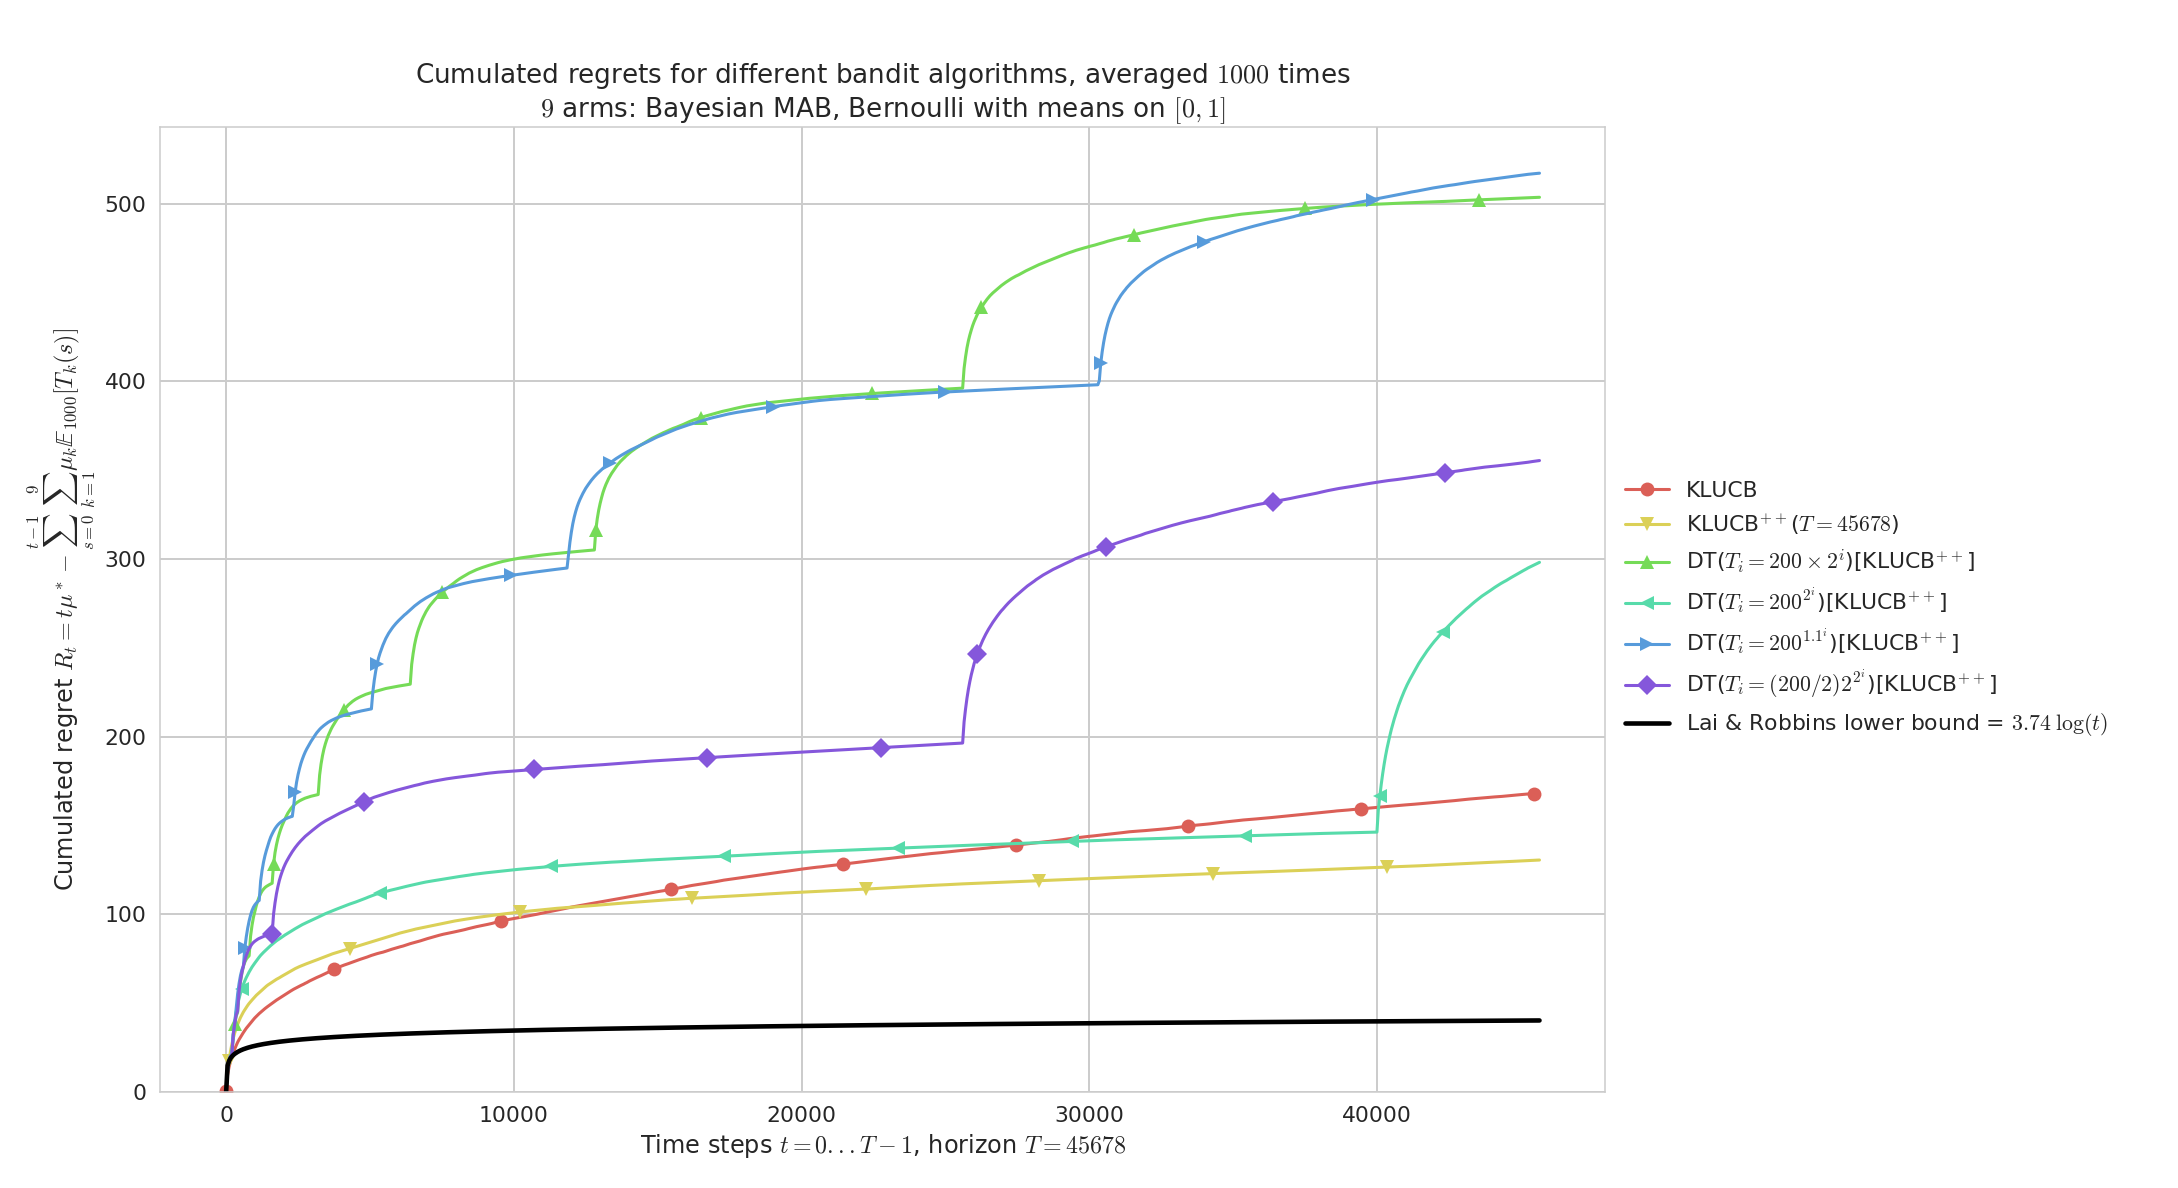
\includegraphics[width=0.95\textwidth]{figures/main____env1-1_1217677871459230631.pdf}
    % \end{subfigure}
    % % ~
    % \begin{subfigure}[!h]{0.49\textwidth}
    %   \includegraphics[width=10092textwidth]{XXX.pdf}
    % \end{subfigure}
    \caption{Regret for \DT, for $K=9$ Bernoulli arms, horizon $T=45678$, $n=1000$ repetitions and $\boldsymbol{\mu}$ taken uniformly in $[0,1]^K$. Geometric doubling ($b=2$) and slow exponential doubling ($b=1.1$) are too slow, and short first sequences make the regret blow up in the beginning of the experiment. At $t=40000$ we see clearly the effect of a new sequence for the best doubling trick ($T_i = 200 \times 2^i$). As expected, \KLUCBpp{} outperforms \KLUCB, and if the doubling sequence is growing fast enough then $\DT(\KLUCBpp)$ can perform as well as \KLUCB{} (see for $t < 40000$).}
    \label{fig:bernoulliBandits_DoublingTrick_Restart_BayesianProblem}
    % \vspace*{-15pt}  % XXX remove if problem
\end{figure}

%
% Regular plots of centralized regrets
%
\begin{figure}[H]
    \centering
    % \begin{subfigure}[!h]{0.49\textwidth}
    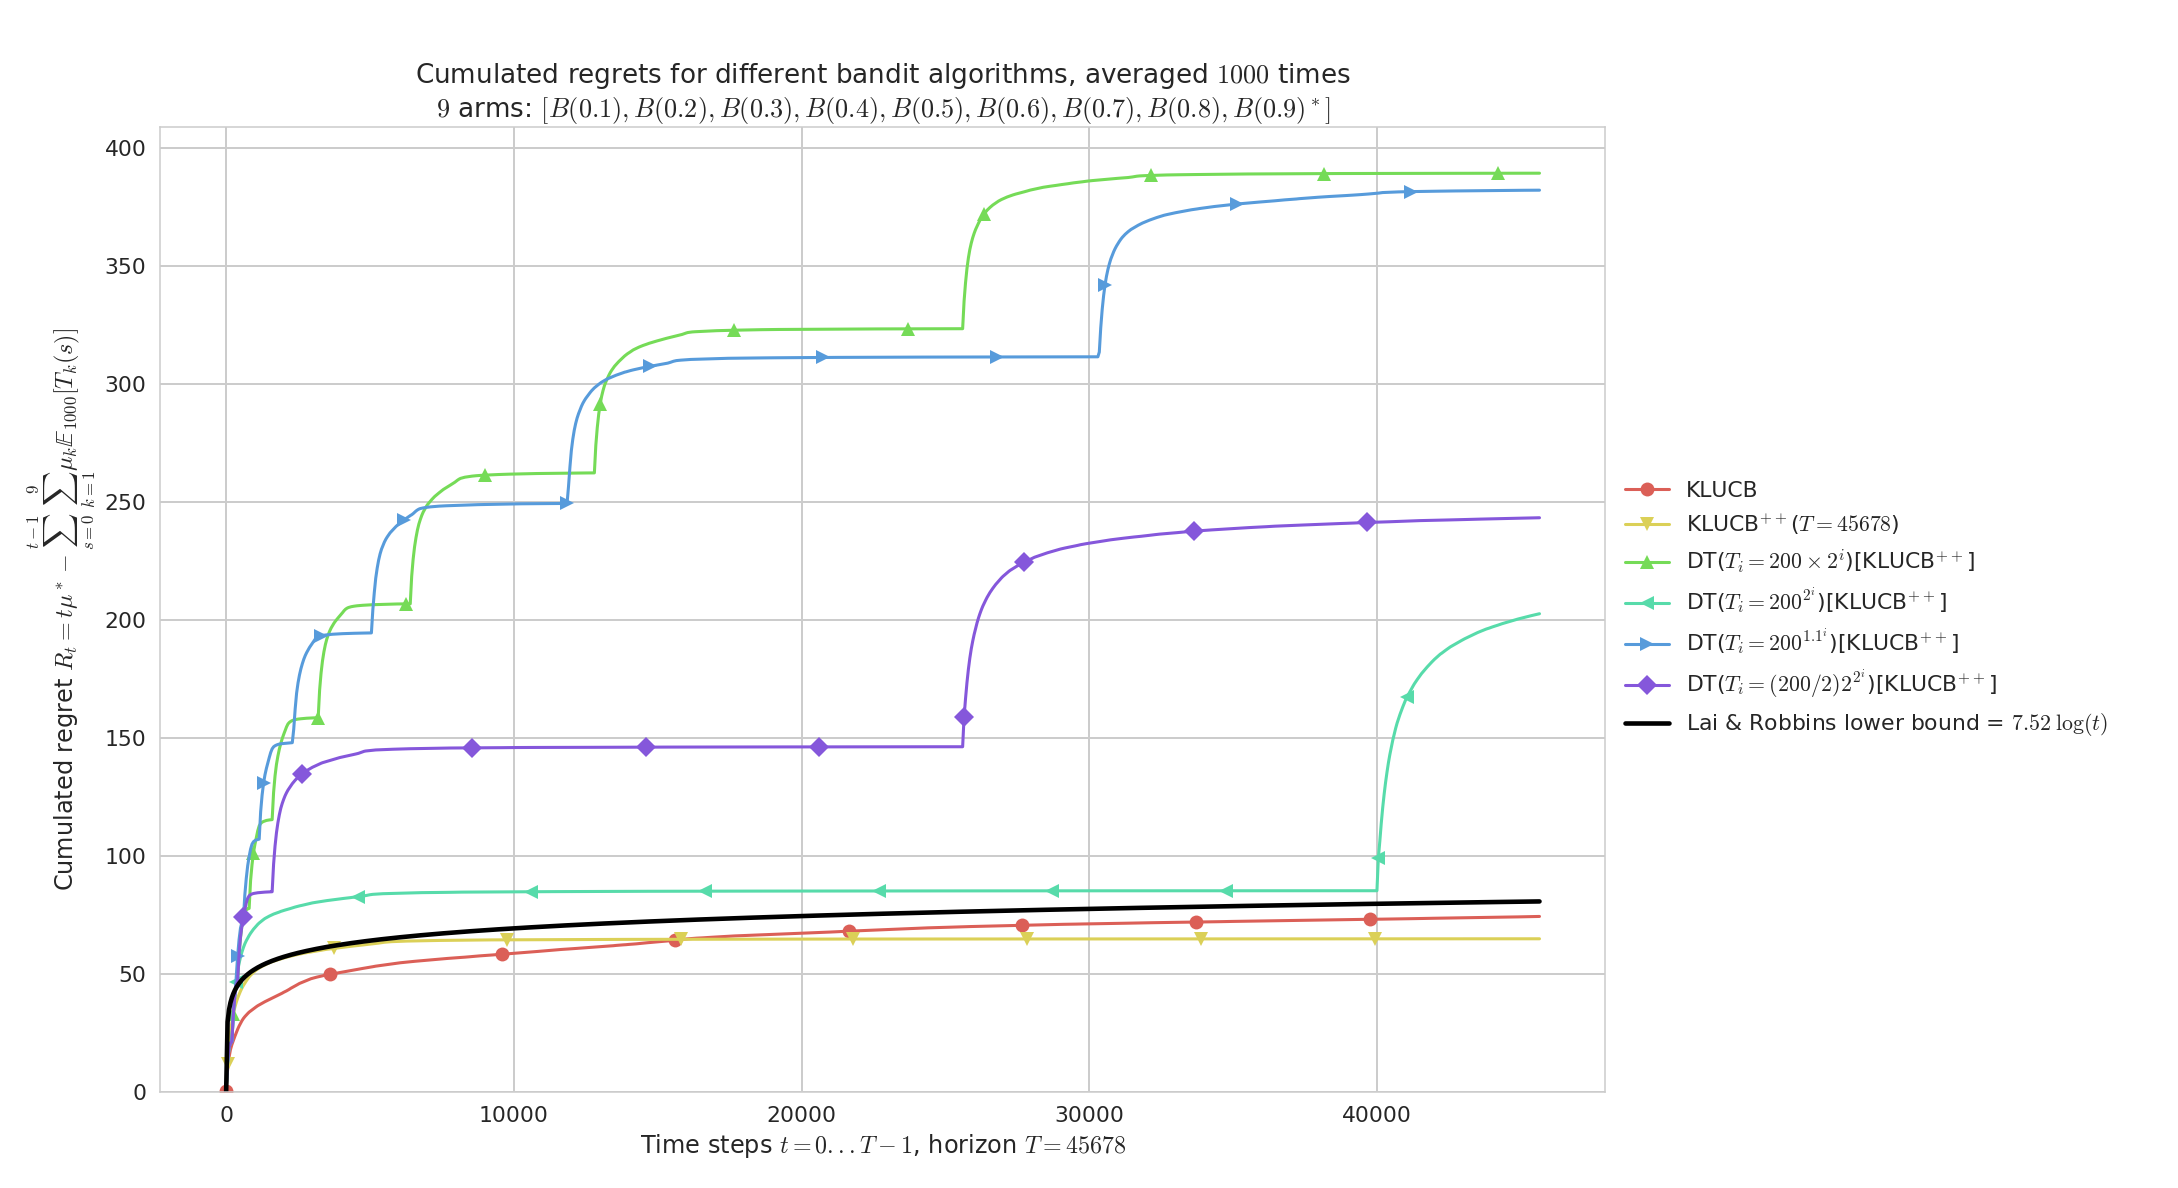
\includegraphics[width=0.93\textwidth]{figures/main____env1-1_3633169128724378553.pdf}
    % \end{subfigure}
    % % ~
    % \begin{subfigure}[!h]{0.49\textwidth}
    %   \includegraphics[width=10092textwidth]{XXX.pdf}
    % \end{subfigure}
    \caption{Similarly but for $\boldsymbol{\mu}$ evenly spaced in $[0,1]^K$ ($\{0.1,\dots,0.9\}$). Both \KLUCB{} and \KLUCBpp{} are very efficient on ``easy'' problems like this one, and we can check visually that they match the lower bound from \cite{LaiRobbins85}. As before we check that slow doubling are too slow to give reasonable performance.}
    \label{fig:bernoulliBandits_DoublingTrick_Restart_fixedProblem}
    \vspace*{-15pt}  % XXX remove if problem
\end{figure}
%
%
% Regular plots of centralized regrets
%
\begin{figure}[!h]
    \centering
    % \begin{subfigure}[!h]{0.49\textwidth}
    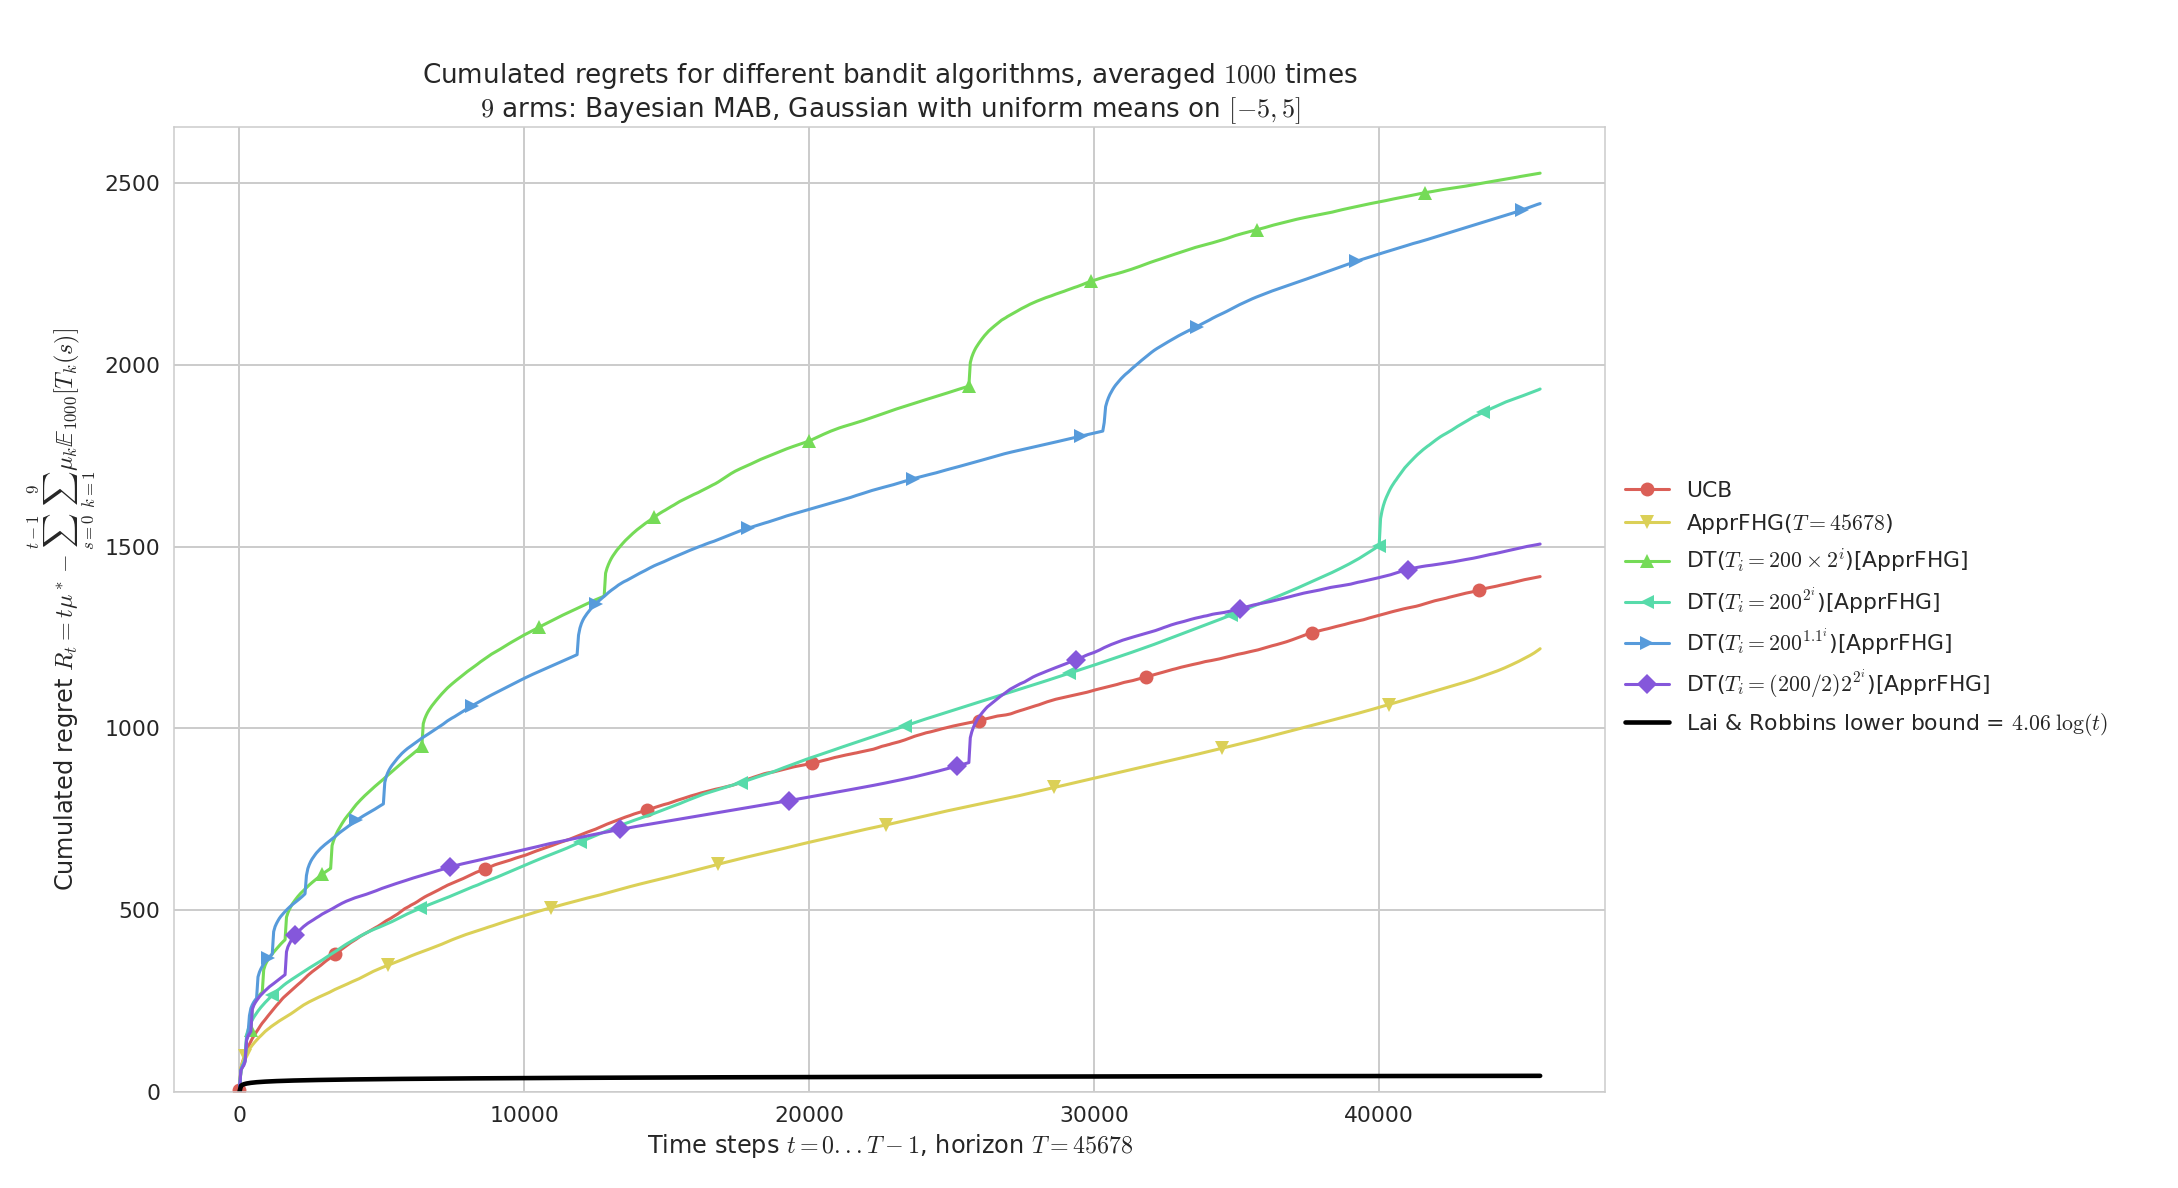
\includegraphics[width=0.93\textwidth]{figures/main____env1-1_2223860464453456415.pdf}
    % \end{subfigure}
    % % ~
    % \begin{subfigure}[!h]{0.49\textwidth}
    %   \includegraphics[width=1.00\textwidth]{XXX.pdf}
    % \end{subfigure}
    \caption{Regret for $K=9$ Gaussian arms $\cN(\mu, 1)$, horizon $T=45678$, $n=1000$ repetitions and $\boldsymbol{\mu}$ taken uniformly in $[-5,5]^K$ and variance $V=1$. On ``hard'' problems like this one, both \UCB{} and \AFHG{} perform similarly and poorly \emph{w.r.t.} to the lower bound from \cite{LaiRobbins85}. As before we check that geometric doubling ($b=2$) and slow exponential doubling ($b=1.1$) are too slow, but a fast enough doubling sequence does give reasonable performance for the anytime \AFHG{} obtained by Doubling Trick.}
    \label{fig:gaussianBandits_DoublingTrick_Restart_fixedProblem}
    % \vspace*{-15pt}  % XXX remove if problem
\end{figure}


% % \FIXME{For a newpage to not have the references starting in a ugly place}
% \clearpage
% \newpage

% -----------------------------------------------------------------
% Acknowledgments---Will not appear in anonymized version
\acks{
    This work is supported
    by the French National Research Agency (ANR), under the project BADASS (grant coded: \texttt{N ANR-16-CE40-0002}),
    % by CentraleSupélec,
    % by the CNRS, under the PEPS project BIO,
    by the French Ministry of Higher Education and Research (MENESR) and {\'E}cole Normale Sup{\'e}rieure Paris-Saclay.
    %
    %Thanks to Odalric-Ambrym Maillard and Florian Strub at Inria Lille for useful discussions.
    %
    The authors wish to thank the anonymous reviewers for their valuable comments that helped to improve the paper.
}

% -----------------------------------------------------------------
% \phantom{\cite{Lattimore16b}}

\bibliography{doublingTrick}
% \nocite{*}  % XXX remove at the end, to only include quoted references!


% \iffalse
\vskip 0.2in
% XXX Remove if problem?
\hr{}
% \vfill{}
\emph{Note}:
    the simulation code used for the experiments is using Python 3.
    % https://www.Python.org/
    It is open-sourced at \verb|https://GitHub.com/SMPyBandits/SMPyBandits|
    %  but is available upon request,
    and fully documented at \newline
    \verb|https://SMPyBandits.GitHub.io|.
    %~\citep{SMPyBandits}.
% \fi
% \hr{}

\clearpage
\newpage

% -----------------------------------------------------------------
\appendix


% -----------------------------------------------------------------
\section{Omitted Proofs}\label{sec:missingproofs}

We include here the proofs omitted in the main document.


\subsection{Proof of Lemma~\ref{lem:decomposition}, ``Regret Lower and Upper Bounds for \DTr''}\label{sub:proof_decompositionDTr}


    Let $\cA'$ denote $\DTr(\cA, (T_i)_{i\in\N})$. For every $k\in \{1,\dots, K\}$,
    \begin{align*}
        & \E\left[\sum_{t=1}^T (X_{k,t} - X_{A(t),t})\right] = \sum_{i=0}^{L_T -1} \E\left[\sum_{t=T_{i-1}}^{T_i}(X_{k,t} - X_{A(t),t})\right] +  \E\left[ \sum_{t=T_{L_T-1}}^{T}(X_{k,t} - X_{A(t),t})\right] \\
        & \hspace{0.7cm} \leq
        \sum_{i=0}^{L_T -1} \max_{k \in \{1,\dots,K\}}\E\left[\sum_{t=T_{i-1}}^{T_i} (X_{k,t} - X_{A(t),t})\right] + \max_{k \in \{1,\dots,K\}}\E\left[ \sum_{t=T_{L_T-1}}^{T}(X_{k,t} - X_{A(t),t})\right] \\
        & \hspace{0.7cm} \leq
        \sum_{i=0}^{L_T -1}R_{T_i-T_{i-1}}\left(\cA'\right) + R_{T - T_{L_T-1}}\left(\cA'\right).
    \end{align*}

    Thus, by definition of the regret
    \begin{align*}
        R_T(\cA')
        &\leq
        \sum_{i=0}^{L_T-1} R_{T_i - T_{i-1}}(\cA')+ R_{T - T_{L_T-1}}(\cA') \\
        &=
        \sum_{i=0}^{L_T-1} R_{T_i - T_{i-1}}\left(\cA_{T_{i} - T_{i-1}}\right)
        + R_{ \underbrace{T - T_{L_T-1}}_{\leq T_{L_T} - T_{L_T-1}} }\left(\cA_{T_{L_T} - T_{L_{T-1}}}\right) \\
        &\leq
        \sum_{i=0}^{L_T} R_{T_i - T_{i-1}}\left(\cA_{T_{i} - T_{i-1}}\right).
    \end{align*}

    In the stochastic case, it is well known that the regret can be rewritten in the following way, introducing $\mu_k$ the mean of arm $k$ and $\mu^*$ the mean of the best arm:
    \begin{align*}
        R_T(\cA') &=
        \E\left[\sum_{t=1}^{T}(\mu^* - \mu_{A(t)})\right] \\
        &=
        \sum_{i=0}^{L_{T-1}} \E\left[\sum_{t=T_{i-1}}^{T_i}(\mu^* - \mu_{A(t)})\right] + \E\left[\sum_{t=T_{L_T-1}}^{T}(\mu^* - \mu_{A(t)})\right] \\
        &=
        \sum_{i=0}^{L_T-1} R_{T_i - T_{i-1}}\left(\cA_{T_i - T_{i-1}}\right)) + \underbrace{R_{T - T_{L_T-1}}(\cA')}_{\geq 0}.
    \end{align*}
    and the lower bound follows.
\hfill{}
$\blacksquare$

\newpage

%     By definition of the regret (Eq.\ref{eq:regret}),
%     and without any \iid{} hypothesis on the rewards,
%     let $\cA'$ denotes $\DTr(\cA, (T_i)_{i\in\N})$.
%     As the $\max$ of a sum is bounded by the sum of the $\max$,
%     we can split the sum on $t\in\{1,\dots,T\}$ on the discrete intervals $\{T_{i-1}, \dots, T_i-1\}$ for $i=0,\dots,L_T-1$ and for $\{T_{L_T-1}, \dots, T-1\}$ for the last sequence\footnote{Beware that it is of course $\cA_{T = T_{L_T} - T_{L_T-1}}$ that is used on the last sequence, and not $\cA_{T = T - T_{L_T-1}}$ as the later would need to use the (unknown) horizon $T$.}, and so
%     % then if
%     % $\cR(t)$ denote the instantaneous regret at time $t$,
%     % $\cR(t) := \sum_{k=1}^K (\max_j \mu_j^{(t)} - \mu_k^{(t)}) \Pr_{\cF_{t-1}}\left[ A'(t) = k \right]$,
%     % We have
%     \begin{align*}
%         R_T(\cA')
%         % &\leq \sum_{t=1}^{T} \cR(t),
%         % &\leq \sum_{i=0}^{L_T-1} \sum_{t=T_{i-1}}^{T_i - 1} \cR(t) + \sum_{t=T_{L_T-1}}^{T} \cR(t)
%         &\leq
%         \sum_{i=0}^{L_T-1} R_{T_i - T_{i-1}}(\cA')
%         + \underbrace{R_{T - T_{L_T-1}}(\cA')}_{:= S \geq 0}.
%         % \intertext{
%         %     So to get the identity leading to Eq.~\eqref{eq:decompositionIneq_UB}, one simply has to observe that, by definition of the algorithm $\DTr$, on each of these sequences
%         %     (for $i\in\{0,\dots,L_T\}$),
%         %     $\cA'$ is exactly $\cA_{T_i-T_{i-1}}$ with its internal timer using $t-T_{i-1}$ instead of $t$ (cf. Algorithm~\ref{algo:DTr}, Line~\ref{line:internalTimer_DTr}).
%         %     % The \iid{} hypothesis on the rewards and the fact that we fully restart the algorithm gives
%         %     % $\Pr_{\bmu}\left[ A'(t) = k \right] = \Pr_{\bmu}\left[ A_{T_i-T_{i-1}}(t-T_{i-1}) = k \right]$
%         %     % if $t\in\{T_{i-1}, \dots, T_i-1\}$.
%         % }
%         % R_T(\cA') &\leq
%         % \sum_{i=0}^{L_T-1} R_{T_i - T_{i-1}}(\cA_{T = T_i - T_{i-1}})
%         % + \underbrace{R_{T - T_{L_T-1}}(\cA_{T = T_{L_T} - T_{L_T-1}})}_{:= S \geq 0}
%     \end{align*}
%     So to get Eq.~\eqref{eq:decompositionIneq_UB}, one simply has to observe that, by definition of the algorithm $\DTr$, on each of these sequences
%     (for $i\in\{0,\dots,L_T\}$),
%     $\cA'$ is exactly $\cA_{T_i-T_{i-1}}$ with its internal timer using $t-T_{i-1}$ instead of $t$ (cf. Algorithm~\ref{algo:DTr}, Line~\ref{line:internalTimer_DTr}).
%     % First, we lower bound the last sum $S$ by $0$ to get the lower bound $(LB)$.
%     % \implies R_T(A') &\underset{LB}{\geq} \sum_{i=0}^{L_T-1} R_{T_i - T_{i-1}}(A_{T = T_i - T_{i-1}}).
%     We bound $S$ by a sum on a \emph{longer} interval, up to $T_{L_T} > T$, as each term in $S$ is non-negative.
%     % ($(\max_j \mu_j^{(t)} - \mu_k^{(t)}) \Pr_{\bmu}\left[ A'(t) = k \right] \geq 0$).
%     % R_T(A')
%     % &\leq \sum_{i=0}^{L_T} \sum_{t=0}^{T_i - T_{i-1}} \sum_{k=1}^K (\max_j \mu_j^{(t)} - \mu_k^{(t)}) \Pr_{\bmu}\left[ A_{T_i-T_{i-1}}(t) = k \right] \\
%     % \implies R_T(A') &\underset{UP}{\leq} \sum_{i=0}^{L_T} R_{T_i - T_{i-1}}(A_{T = T_i - T_{i-1}}).
%
%     Now for the stochastic case, the \iid{} hypothesis on the reward make the first inequality above an equality, as the $\max$ and the expectation can be exchanged.
%     For the lower bound Eq.~\eqref{eq:decompositionIneq_LB}, we simply have to observe that $S \geq 0$.
% \end{proof}

% \paragraph{Remark.}
% Note that the lower bound becomes looser when $T$ gets closer to $T_{L_T}-1$, and conversely the upper bound becomes looser when $T$ gets closer to $T_{L_T-1}$.


% \subsection{Proof of Theorem~\ref{thm:keep4}}\label{sub:proof_keep4}


% \begin{proof}\label{proof:Keep4}
%     Let $A' := \DTr(A, (T_i)_{i\in\N})$.
%     We start by using Lemma~\ref{lem:decomposition},
%     % we get a decomposition on the regret of $A$ for time $T$ as a sum of regrets on sequences of successive lengths $T_i - T_{i-1}$, so
%     \begin{align*}
%         R_T(A')
%         &\leq \sum_{i=0}^{L_T} R_{T_i - T_{i-1}}(A_{T = T_i - T_{i-1}}) \\
%         \intertext{
%             We bound $T_i - T_{i-1} \leq 1 + T_0 (b - 1) b^{i-1}$ for $i>0$, thanks to Definition~\ref{def:geomSequence},
%             and we can use the hypothesis on $A$ for each regret term,
%             as $t \mapsto c t^{\gamma}$ and $f$ are non-decreasing for $t\geq 1$ (as $\gamma>0$).
%             Additionally,
%             $(T_i - T_{i-1})^{\gamma} \leq 1 + T_0^{\gamma} (b - 1)^{\gamma} (b^{i-1})^{\gamma}$ by Lemma~\ref{lem:expoInequality} (Eq.~\eqref{eq:expoInequality1}, as $\gamma<1$), thus
%         }
%         &\leq \sum_{i=0}^{L_T} c (T_i - T_{i-1})^{\gamma} + f(T_i - T_{i-1})
%         \leq \sum_{i=0}^{L_T} f(T_i) + c T_0^{\gamma} \sum_{i=1}^{L_T} c (T_i - T_{i-1})^{\gamma} \\
%         &\leq \left[\sum_{i=0}^{L_T} f(T_i) + c (T_0^{\gamma} + L_T)\right] + c T_0^{\gamma} (b - 1)^{\gamma} \sum_{i=1}^{L_T} (b^{i-1})^{\gamma} \\
%         \intertext{
%             The first part is denoted $g(T):=\sum_{i=0}^{L_T} f(T_i) + c (T_0^{\gamma} + L_T)$, and is an increasing function as a sum of increasing functions.
%             By Lemma~\ref{lem:ControlLemmaSumOfSmallO}, the sum of $f(T_i)$ is a $\smallO{\sum_{i=0}^{L_T} T_i^{\gamma}}$, as $f(t) = \smallO{t^{\gamma}}$ by hypothesis, and this sum of $T_i^{\gamma}$ is proved below to be bounded by $c' T^{\gamma}$ for a certain constant $c'>0$.
%             Moreover, $L_T = \bigO{\log T} = \smallO{T^{\gamma}}$ (for any $\gamma>0$),
%             so $g(t)$ is $\smallO{t^{\gamma}}$ as wanted.
%             %
%             We bound the second part by $\sum_{i=0}^{L_T-1} (b^i)^{\gamma} \leq \frac{1}{b^{\gamma} - 1} (b^{L_T})^{\gamma}$ thanks to a geometric sum and thus
%         }
%         &\leq g(T) + c T_0^{\gamma} \frac{(b - 1)^{\gamma}}{b^{\gamma} - 1} (b^{L_T})^{\gamma}
%         \intertext{
%             We see that $b^{L_T} = b b^{L_T - 1}$, and $b^{L_T - 1} \leq \frac{T}{T_0}$ also thanks to Definition~\ref{def:geomSequence}, so
%         }
%         &\leq g(T) + c T_0^{\gamma} \frac{b^{\gamma} (b - 1)^{\gamma}}{b^{\gamma} - 1} \frac{T^{\gamma}}{T_0^{\gamma}}
%         = g(T) + \frac{b^{\gamma} (b - 1)^{\gamma}}{b^{\gamma} - 1} \; c T^{\gamma} \\
%         \implies R_T(A') &\leq g(T) + \ell(\gamma, b) \; c T^{\gamma} \text{ with an increasing } g(T) = \smallO{T^{\gamma}}.
%     \end{align*}

%     To minimize this constant overhead $\ell(\gamma, b) = \frac{b^{\gamma} (b - 1)^{\gamma}}{b^{\gamma} - 1} > 1$, we fix $\gamma$ and study $h: b \mapsto \ell(\gamma, b)$.
%     The function $h$ is of class $\cC^1$ on $(1, \infty)$ and $h(b) \to +\infty$ for $b\to 1^+$ and $b\to\infty$,
%     so $h$ has a (possibly non-unique) global minimum and attains it.
%     Moreover $h'(b) = \frac{\gamma b^{\gamma-1} (b-1)^{\gamma-1}}{(b^{\gamma}-1)^2} \left( b^{\gamma+1} - 2 b + 1 \right)$ has the sign of $b^{\gamma+1} - 2 b + 1$,
%     which does not have a constant sign and does not have explicit root(s) for a generic $\gamma$.
% \end{proof}


\subsection{Proof of Theorem~\ref{thm:keep45}, ``Conserving a Regret Upper Bound with Geometric Horizons''}\label{sub:proof_keep45}

It is interesting to note that
the proof is valid for both the easiest case when $\delta=0$ (as it was known in \cite{CesaLugosi06} for $\gamma=1/2$)
and the generic case when $\delta\geq0$,
with no distinction.

As far as the authors know, this result in its generality with $\delta\geq0$ is new.

\vspace*{5pt}  % XXX remove if problem
\begin{proof}\label{proof:Keep45}
    Let $\cA' := \DTr(\cA, (T_i)_{i\in\N})$, and consider a fixed bandit problem.
    % The proof starts exactly like for the previous one for Theorem~\ref{thm:keep4}.
    The upper bound \eqref{eq:decompositionIneq_UB} from Lemma~\ref{lem:decomposition} gives
    \begin{align*}
        R_T(\cA')
        &\leq \sum_{i=0}^{L_T} R_{T_i - T_{i-1}}(A_{T = T_i - T_{i-1}}) \\
        \intertext{
            We can use the hypothesis on $\cA$ for each regret term,
            as $f$ and $t \mapsto c t^{\gamma} (\log t)^{\delta}$ are non-decreasing for $t\geq 1$ (by hypothesis for $f$ and by Lemma~\ref{lem:tgammalogtdeltaIncreasing}).
        }
        &\leq \sum_{i=0}^{L_T} f(T_i - T_{i-1}) + c T_0^{\gamma} (\log T_0)^{\delta}
        + c \sum_{i=1}^{L_T} \left(T_i - T_{i-1}\right)^{\gamma} \left(\log\left(T_i - T_{i-1}\right)\right)^{\delta}
        \intertext{
            The first part is denoted $g_1(T):= \sum_{i=0}^{L_T} f(T_i - T_{i-1}) + c T_0^{\gamma} (\log T_0)^{\delta}$, it is an increasing function as a sum of increasing functions, and it is dealt with by using Lemma~\ref{lem:ControlLemmaSumOfSmallO}:
            the sum of $f(T_i - T_{i-1})$ is a $\smallO{\sum_{i=0}^{L_T} (T_i - T_{i-1})^{\gamma} (\log(T_i - T_{i-1}))^{\delta}}$, as $f(t) = \smallO{t^{\gamma} (\log t)^{\delta}}$ by hypothesis, and this sum of $(T_i - T_{i-1})^{\gamma} (\log(T_i - T_{i-1}))^{\delta}$ is proved below to be bounded by $c' T^{\gamma} (\log T)^{\delta}$ for a certain constant $c'>0$,
            which gives $g_1(T) = \smallO{T^{\gamma} (\log T)^{\delta}}$.
            %
            For the second part,
            we bound $T_i - T_{i-1} \leq T_0 (b-1) b^{i-1} + 1$ thanks to Definition~\ref{def:geomSequence}.
            Moreover, as $\gamma<1$
            we can use Lemma~\ref{lem:expoInequality} (Eq.~\eqref{eq:expoInequality1}) to distribute the power on $\gamma$,
            so $(T_0 (b-1) b^{i-1} + 1)^{\gamma} \leq (T_0 (b-1) b^{i-1})^{\gamma} + \mathbbm{1}(\gamma\neq0)$ (indeed if $\gamma=0$ both sides are equal to $1$).
            This gives
        }
        &\leq g_1(T) + c
            (T_0 (b-1))^{\gamma} \sum_{i=1}^{L_T} (b^{i-1})^{\gamma} \left(\log(T_i - T_{i-1})\right)^{\delta}
            + c \mathbbm{1}(\gamma\neq0) \sum_{i=1}^{L_T} \left(\log(T_i - T_{i-1})\right)^{\delta} \\
        \intertext{
            If $\gamma\neq 0$,
            the last sum is bounded by $\sum_i^{L_T} (\log T_i)^{\delta} \leq (\log T_0)^{\delta}(L_T + 1) + (\log b)^{\delta} \sum_i^{L_T} i^{\delta}$ which is a $\bigO{L_T^{\delta+1}} = \bigO{(\log T)^{\delta+1}} = \smallO{T^{\gamma} (\log T)^{\delta}}$ (as $\gamma>0$, thanks to a geometric sum), and so it can be included in $g_2(T) = \smallO{T^{\gamma} (\log T)^{\delta}}$.
            If $\gamma=0$, there is only the first sum.
            %
            We bound again $T_i - T_{i-1} \leq T_0 (b-1) b^{i-1} + 1$
            and use Lemma~\ref{lem:logxm1_logx} to bound $\log(T_0 (b-1) b^{i-1} + 1)$
            by $\frac{\log(T_0 (b-1) + 1)}{\log(T_0 (b-1))} \log(T_0 (b-1) b^{i-1}) $ term (as $T_0 (b-1) > 1$ by hypothesis).
        }
        &\leq g_2(T) + c
            (T_0 (b-1))^{\gamma} \sum_{i=1}^{L_T} (b^{i-1})^{\gamma} \left( \frac{\log(T_0 (b-1) + 1)}{\log(T_0 (b-1))} \log(T_0 (b-1) b^{i-1})\right)^{\delta} \\
        \intertext{
            We split the $\log(T_0(b-1)b^{i-1})$ term in two, and
            once again, the term with $\log(T_0(b-1))$ gives a $\bigO{{b^{L_T-1}}}$ (by a geometric sum), which gets included in $g_3(T) = \smallO{T^{\gamma} (\log T)^{\delta}}$.
            We focus on the fastest term, and we can now rewrite the sum from $i=0$ to $L_T-1$,
        }
        &\leq g_3(T) + c
            (T_0 (b-1))^{\gamma} \left(\log(b) \frac{\log(T_0 (b-1) + 1)}{\log(T_0 (b-1))} \right)^{\delta} \sum_{i=0}^{L_T-1} (b^i)^{\gamma} i^{\delta} \\
        \intertext{
            We naively bound $i^{\delta}$ by $(L_T-1)^{\delta}$,
            and use a geometric sum
            % Corollary~\ref{cor:SumIneq3} (Eq.~\eqref{eq:sum_igamma_bidelta})
            to have
        }
        &\leq g_3(T) + c
            (T_0 (b-1))^{\gamma} \left(\log(b) \frac{\log(T_0 (b-1) + 1)}{\log(T_0 (b-1))} \right)^{\delta} (L_T-1)^{\delta} \frac{b^{\gamma}}{b^{\gamma}-1} (b^{L_T-1})^{\gamma} \\
        \intertext{
            Finally, observe that $L_T-1 \leq \log_b(\frac{T}{T_0}) \leq \log_b(T)$, so the $(\log b)^{\delta}$ term simplifies,
            and observe that $b^{L_T-1} \leq \frac{T}{T_0}$ so the $T_0^{\gamma}$ term also simplifies.
            Thus we get
        }
        &\leq g_3(T) + c
            \left(\frac{\log(T_0 (b-1) + 1)}{\log(T_0 (b-1))} \right)^{\delta} \frac{b^{\gamma} (b-1)^{\gamma}}{b^{\gamma}-1} T^{\gamma} (\log T)^{\delta}.
    \end{align*}

    The constant multiplicative overhead $\ell$ depends on $\gamma$ and $\delta$ as well as on $T_0$ and $b$,
    and is
    $\ell(\gamma, \delta, T_0, b) := \left(\frac{\log(T_0 (b-1) + 1)}{\log(T_0 (b-1))} \right)^{\delta} \frac{b^{\gamma} (b-1)^{\gamma}}{b^{\gamma}-1} > 1$.
\end{proof}


\paragraph{Minimizing the constant overhead?}
%
This constant overhead has two distinct part,
$\ell(\gamma, \delta, T_0, b) = \ell_1(\delta, T_0, b)$ $\ell_2(\gamma, b)$,
with $\ell_1$ depending on $\delta$, $T_0$ and $b$ (equal to $1$ if $\delta=0$),
and $\ell_2$ depending on $\gamma$ and $b$.
\begin{itemize}
    \item
Minimizing this constant overhead $\ell_1(\delta, T_0, b) := \left(\frac{\log(T_0 (b-1) + 1)}{\log(T_0 (b-1))} \right)^{\delta}\geq 1$ is independent of $\delta$ (even if it is $0$).
If we assume $b$ to be fixed,
% (as a value is suggested by minimizing $\ell_2(\gamma, b)$),
$\ell_1(\delta, T_0, b) \to 1$ when $T_0\to\infty$.
Moreover, for any $\delta$ and $b>1$,
$\ell_1(\delta, T_0, b)$ goes to $1$ very quickly when $T_0$ is large enough.
For instance, for $\gamma=\delta=\frac{1}{2}$ and $b=\frac{3+\sqrt{5}}{2}$ (see Corollary~\ref{cor:keep4}),
then $\ell_1(\delta, T_0, b) \simeq 1.109$ for $T_0=2$, $\simeq 1.01$ for $T_0=10$ and $\simeq 1.0004$ for $T_0=100$.
    \item
To minimize this constant overhead $\ell_2(\gamma, b) := \frac{b^{\gamma} (b - 1)^{\gamma}}{b^{\gamma} - 1} > 1$, we fix $\gamma$ and study $h: b \mapsto \ell_2(\gamma, b)$.
The function $h$ is of class $\cC^1$ on $(1, \infty)$ and $h(b) \to +\infty$ for $b\to 1^+$ and $b\to\infty$,
so $h$ has a (possibly non-unique) global minimum and attains it.
Moreover $h'(b) = \frac{\gamma b^{\gamma-1} (b-1)^{\gamma-1}}{(b^{\gamma}-1)^2} \left( b^{\gamma+1} - 2 b + 1 \right)$ has the sign of $b^{\gamma+1} - 2 b + 1$,
which does not have a constant sign and does not have explicit root(s) for a generic $\gamma$.
%
However, it is easy to minimizing $\ell_2(\gamma, b)$ for $b$ numerically when $\gamma$ is known and fixed (with, \eg, Newton's method).
\end{itemize}

% XXX To minimize it, we fix $\gamma$ and study $h: x \mapsto \frac{x^2}{x - 1}$.
% The function $h$ is of class $\cC^1$ on $(1, \infty)$ and $h(b) \to +\infty$ for $b\to 1^+$ and $b\to\infty$,
% so $h$ has a (possibly non-unique) global minimum and attains it.
% Moreover $h'(x) = \frac{x}{(x-1)^2}(x-2)$ has the sign of $x-2$, so $h$ is convex
% and has a unique global minimum attained at $x^*=2$.
% At this point, $h(x^*) = \frac{(x^*)^2}{x^* - 1} = 4$.
% % Moreover $h'(b) = \frac{b^{\gamma - 1} \gamma}{(\log(b^{\gamma}))^2} \left( (\log(b^{\gamma}))^2 + \log(b^{\gamma}) - 1 \right)$ has the sign of $y^2 + y - 1$ (if $y := \log(b^{\gamma}) > 0$).
% % The polynomial $y^2 - y + 1$ has a unique root on $(0, +\infty)$, $y_0 := \frac{\sqrt{5} - 1}{2} \simeq 0.618$.
% % Thus, as $x_0 := \exp(y_0) > 1$, $h$ has a unique global minimum, attained for $b^*(\gamma) = x_0^{1/\gamma} = \exp(\frac{y_0}{\gamma}) > 1$.
% % At this point, $h(b^*(\gamma)) = x_0 (1 + \frac{1}{x_0}) = \exp\left(\frac{\sqrt{5} - 1}{2}\right) \left( \frac{\sqrt{5} + 1}{\sqrt{5} - 1}\right) \simeq 4.86 > 1$.
% %
% % Note that this constant is larger than the minimum found in the previous Theorem~\ref{thm:keep4}, as we were less subtle in the inequalities.


The result from Theorem~\ref{thm:keep45} of course implies the result from \cite[Ex.2.9]{CesaLugosi06}, in the special case of $\delta=0$ and $\gamma=\frac{1}{2}$ (for minimax bounds),
as stated numerically in the following Corollary~\ref{cor:keep4}.

\begin{corollary}\label{cor:keep4}
    If $\gamma=\frac{1}{2}$ and $\delta=0$,
    the multiplicative overhead $\ell(\frac{1}{2}, 0, T_0, b)$ does not depend on $T_0$.
    It is then minimal for $b^*(\frac{1}{2}) = \frac{3 + \sqrt{5}}{2} \simeq 2.62$ and its minimum is $\sqrt{\frac{11 + 5 \sqrt{5}}{2}} \simeq 3.33$.
    Usually $b = 2$ is used, which gives an overhead of $\frac{\sqrt{2}}{\sqrt{2} - 1} \simeq 3.41$, close to the optimal value.

    % If $c_1 \neq 0$, the optimal value $b^*$ for the parameter $b$ depends on $c_1$ and $c_1'$ but not on $T_0$, so it can still be computed for known values of $c_1,c_1'$.
    % There is a tradeoff between the term $\frac{2}{\e \log(b)}$ in front of $c_1$ (which goes to $\infty$ for $b\to 1$ and $0$ for $b\to\infty$) and the term in front of $c_1'$ (which goes to $\infty$ for $b\to\infty$), and a global minimum $b^*$ always exist and is unique, but a closed form is less helpful.

    In particular, order-optimal and optimal algorithms for the minimax bound
    have $\gamma=\frac{1}{2}$ and $f(t)=0$,
    for which Theorem~\ref{thm:keep52} gives a simpler bound
    \begin{equation}\label{eq:corkeep4_1}
        % \forall T \geq 1,\;\;\;\;
        R_T(\cA_T) \leq c \sqrt{T}
        \implies
        R_T(\DTr(\cA, (T_0 2^i)_{i\in\N})) \leq \frac{\sqrt{2}}{\sqrt{2} - 1} c \sqrt{T}.
    \end{equation}
\end{corollary}




% \subsection{XXX}

% % \FIXME{Celui là est bon est intéressant. Mais ça ne révolutionne rien. Par contre il est très propre puisqu'on trouve la même overhead que dans le théorème \ref{thm:keep4} avec geometric sequences for $\sqrt{T}$ bounds.}


% \begin{theorem}\label{thm:keep5}
%     If an algorithm $A$ satisfies
%     $ R_T(A) \leq c (\log T)^{\delta}+ f(t)$,
%     for $\delta > 0$,
%     and for $c > 0$, and an increasing function $f(t) = \smallO{(\log t)^{\delta}}$ (at $t\to\infty$),
%     then the anytime version $A':=\DTr(A, (T_i)_{i\in\N})$ with the exponential sequence $(T_i)_{i\in\N}$ of parameters $T_0\in\N^*,a,b>1$ (\ie, $T_i = \lfloor \frac{T_0}{a} a^{b^i}\rfloor$),
%     satisfies the following inequality
%     \begin{equation}\label{eq:keep5_1}
%         \forall T \geq 1,\;\;\;\;
%         R_T(A') \leq \ell(\delta, b) \; c \; (\log T)^{\delta} + g(T).
%     \end{equation}
%     with an increasing function $g(t) = \smallO{(\log T)^{\delta}}$,
%     and a \emph{constant overhead} $\ell(\delta, b) > 1$
%     \begin{equation}\label{eq:keep5_2}
%         \ell(\delta, b) :=
%         \frac{b^{2\delta}}{b^{\delta} - 1} \geq 4.
%     \end{equation}

%     $\ell(\delta, b)$ is minimal at $b^*(\delta) = 2^{1/\delta} > 1$
%     and for a minimal value of $\min\limits_{b > 1} \ell(\delta, b) = 4$ (\textbf{for any} $\delta$).
% \end{theorem}


% \FIXME{Move the proof in Appendix? It's not that different from the previous one...}
% \begin{proof}\label{proof:Keep5}
%     Let $A' := \DTr(A, (T_i)_{i\in\N})$.
%     The proof starts like for the previous ones for Theorem~\ref{thm:keep45}.
%     \begin{align*}
%         R_T(A')
%         &\leq \sum_{i=0}^{L_T} R_{T_i - T_{i-1}}(A_{T = T_i - T_{i-1}}) \\
%         \intertext{
%             We bound naively $T_i - T_{i-1} \leq T_i \leq \frac{T_0}{a} a^{b^i}$,
%             and we can use the hypothesis on $A$ for each regret term,
%             as $f$ and $t \mapsto c  (\log t)^{\delta}$ are non-decreasing for $t\geq 1$ (by hypothesis for $f$ and by Lemma~\ref{lem:tgammalogtdeltaIncreasing}).
%         }
%         &\leq \sum_{i=0}^{L_T} f(T_i) + c \sum_{i=0}^{L_T} \left(\log\left(T_i\right)\right)^{\delta}
%         \leq g_1(T) + c \sum_{i=0}^{L_T} \left(\log\left(\frac{T_0}{a} a^{b^i}\right)\right)^{\delta} \\
%         \intertext{
%             The first part is denoted $g_1(T):= \sum_{i=0}^{L_T} f(T_i)$ and is dealt with Lemma~\ref{lem:ControlLemmaSumOfSmallO}.
%             The sum of $f(T_i)$ is a $\smallO{\sum_{i=0}^{L_T} (\log(T_i))^{\delta}}$, as $f(t) = \smallO{(\log t)^{\delta}}$ by hypothesis, and this sum of $(\log(T_i))^{\delta}$ is proved below to be bounded by $(\log T)^{\delta}$ for a certain constant $c'>0$.
%             %
%             The second part is $c \sum_{i=0}^{L_T}  \left(\log\left(\frac{T_0}{a} a^{b^i}\right)\right)^{\delta}$.
%             Define $\log^+(x) := \max(\log(x), 0) \geq 0$, so whether $\frac{T_0}{a} \leq 1$ or $ >1$, we always have $\log\left(\frac{T_0}{a} a^{b^i}\right) \leq \log^+\left(\frac{T_0}{a}\right) + \log\left(a^{b^i}\right)$.
%             %
%             Thus we can use Lemma~\ref{lem:expoInequality} (Eq.~\eqref{eq:expoInequality1}) to distribute the power on $\delta$ (as it is $<1$). So $\left(\log\left(\frac{T_0}{a} a^{b^i}\right)\right)^{\delta} \leq \left(\log^+\left(\frac{T_0}{a}\right)\right)^{\delta} + \left(\log(a)\right)^{\delta} \left(b^i\right)^{\delta}$ with $0^{\delta} = 0$ (even if $\delta=0$),
%             and so this gives
%         }
%         &\leq g_1(T) + c \left[
%             \left(\log^+\left(\frac{T_0}{a}\right)\right)^{\delta} (L_T + 1)
%             + \left(\log(a)\right)^{\delta} \sum_{i=0}^{L_T} \left(b^i\right)^{\delta}
%         \right] \\
%         \intertext{
%             For the two terms,
%             we use two results proved in Appendix~\ref{sec:otherproofs}.
%             We know that for the exponential sequence, $L_T = \bigO{\log(\log T)}$ which can be included in $g_1(T) = \smallO{(\log T)^{\delta}}$ (still increasing),
%             and so only the second sum has to be bounded.
%             a geometric sum gives $\sum_{i=0}^{L_T} \left(b^i\right)^{\delta} \leq \left(\frac{b^{\delta}}{b^{\delta} - 1}\right) (b^{L_T})^{\delta} = \left(\frac{b^{2\delta}}{b^{\delta} - 1}\right) (b^{L_T-1})^{\delta}$.
%         }
%         &\leq g_1(T) + c c' (b^{L_T-1})^{\delta} \\
%         \intertext{
%             We identify a constant multiplicative overhead $c' := (\log a)^{\delta} \frac{b^{2\delta}}{b^{\delta} - 1}$.
%             We know that
%             $b^{L_T-1} \leq \log_a(\frac{T}{T_0}) \leq \log_a(T)$ (as $T_0 \geq 1$),
%             and so the $(\log a)^{\delta}$ get cancelled and thus
%         }
%         &\leq g(T) + \frac{b^{2\delta}}{b^{\delta} - 1} c \left(\log T\right)^{\delta} \\
%         \implies R_T(A') &\leq g(T) + \ell(\delta, b) \; c \left(\log T\right)^{\delta} \text{ with an increasing } g(T) = \smallO{\left(\log T\right)^{\delta}}.
%     \end{align*}

%     So the constant multiplicative overhead $\ell$ depends only on $\delta$ and $b$ and is
%     \begin{align*}
%         \ell(\delta, b) :=
%         \frac{b^{2\delta}}{b^{\delta} - 1} \geq 4
%         % \begin{cases}
%         %     1 + \frac{1}{\delta\log(b)} > 1 & \text{~if~} \gamma > 0, \\
%         %     1 + \frac{1}{b^{\delta} - 1} > 1 & \text{~if~} \gamma = 0.
%         % \end{cases}
%     \end{align*}
%     The constant is always larger than its minimum $\min_{b>1} \ell(\delta, b) = \ell(\delta, b^*(\delta)) = 4$, attained for $b = b^*(\delta) = 2^{\frac{1}{\delta}}$.
% \end{proof}


\subsection{Proof of Theorem~\ref{thm:LowerBoundExpo_sqrt}, ``Minimax Regret Lower Bound with Exponential Horizons''}\label{sub:proof_LowerBoundExpo_sqrt}

\begin{proof}\label{proof:LowerBoundExpo_sqrt}
    Let $\cA' := \DTr(\cA, (T_i)_{i\in\N})$, and consider a fixed \emph{stochastic} bandit problem.
    The lower bound \eqref{eq:decompositionIneq_LB} from Lemma~\ref{lem:decomposition} gives
    % The proof starts similarly to the proof of Theorem~\ref{thm:LowerBoundGeom_log}.
    \begin{align*}
        R_T(\cA')
        &\geq \sum_{i=0}^{L_T-1} R_{T_i - T_{i-1}}(A_{T = T_i - T_{i-1}}) \\
        \intertext{
            We can use the hypothesis on $\cA$ for each regret term,
            and as $0 < \gamma \leq 1$, we can use Lemma~\ref{lem:expoInequality} (Eq.~\eqref{eq:expoInequality3}) to distribute the power on $\gamma$ to ease the proof and obtain
        }
        &\geq c T_0^{\gamma} + c \sum_{i=1}^{L_T-1} (T_i - T_{i-1})^{\gamma} \\
        &\geq c T_0^{\gamma} + c \sum_{i=1}^{L_T-1} \left(T_i^{\gamma} - T_{i-1}^{\gamma}\right) \;\;\;\;\text{(it is a telescopic sum and simplifies)} \\
        &\geq c T_{L_T-1}^{\gamma} \\
        \intertext{
            % $(\log (T_{L_T-1}))^{\delta}$
            % \FIXME{Maybe justify more how to handle the $(\log(...))^{\delta}$ term? Je crois que c'est trop rapide en l'état, on doit dire mieux (mais le théorème marche, j'en suis sur).}
            % As the telescopic sum simplifies.
            % and because we bound $\log (T_i - T_{i-1}) \geq \log (T_{L_T-1})$.
            % We bound naively $T_i \geq \frac{T_0}{a} a^{b^i} - \frac{T_0}{a} a^{b^{i-1}} - 1$.
            Observe that
            $T_{L_T-1} \geq (T_{L_T})^{\frac{1}{b}}$ by definition of the exponential sequence (Def.~\ref{def:expSequence}), and $T_{L_T} \geq T$ (Def.~\ref{def:lastTerm}).
            For the $\log (T_{L_T-1})$ term, we simply have $\log (T_{L_T-1}) \geq \frac{1}{b} \log(T)$ so if $c' = c / b$,
            then we obtain what we want
        }
        R_T(\cA')
        &\geq c' \; T^{\frac{\gamma}{b}}.
    \end{align*}
    This lower bound goes from $R_T(\cA_T) = \Omega(T^{\gamma})$ to $R_T(\DT(\cA)) = \Omega(T^{\frac{\gamma}{b}})$,
    and it looks very similar to the upper bound from Theorem~\ref{thm:keep52} where
    $R_T(\DT(\cA)) = \bigO{T^{b\gamma}}$
    was obtained from
    $R_T(\cA_T) = \bigO{T^{\gamma}}$.
\end{proof}

\paragraph{Remark}
It does seem sub-optimal to lower bound $T_{L_T-1}$ like this ($T_{L_T-1} \geq (T_{L_T})^{\frac{1}{b}}$), but we remind that $T$ can be located anywhere in the discrete interval $\{T_{L_T-1}, \dots, T_{L_T} - 1\}$, so in the worst case when $T$ is very close to $T_{L_T}$ (and for large enough $T$), we indeed have $T_{L_T-1}^b \sim T_{L_T}$ and $T_{L_T} \sim T$, so with this approach, the lower bound $T_{L_T-1} \geq T^{\frac{1}{b}}$ cannot be improved.


% -----------------------------------------------------------------

% \hr{}

% \section{Minimax Regret Lower Bound with Geometric Horizons}\label{sub:LowerBoundGeom_sqrt}

% \TODO{Remove, weird statement hard to get for the reader}

% We include here a last result that partly replies to Theorem~\ref{thm:keep45}.
% It is more subtle that the lower bound in Theorem~\ref{thm:LowerBoundGeom_log} but still provides an interesting insight:
% if $b$ is not chosen carefully (\ie, if $\ell_0(\gamma,b) > 1$), then the anytime version of $\cA_T$ using a geometric Doubling Trick suffers a non-improvable constant multiplicative overhead compared to $\cA_T$.

% \begin{theorem}\label{thm:LowerBoundGeom_sqrt}
%     For \emph{stochastic models},
%     if $\cA$ satisfies
%     $ R_T(\cA_T) \geq c \; T^{\gamma}$,
%     for $0<\gamma<1$ and $c > 0$,
%     then the anytime version $\cA':=\DTr(\cA, (T_i)_{i\in\N})$ with the geometric sequence $(T_i)_{i\in\N}$ of parameters $T_0\in\N^*,b>1$ (\ie, $T_i = \lfloor T_0 b^i \rfloor$) satisfies
%     \begin{equation}
%         % \forall T \geq 1,\;\;\;\;
%         L_T \geq 2 \implies
%         R_T(\cA') \geq \ell_0(\gamma, b) \; c \; T^{\gamma} + g_0(T).
%     \end{equation}
%     with $g_0(t) = \bigO{\log t} = \smallO{t^{\gamma}}$,
%     and a \emph{constant overhead} $\ell_0(\gamma, b)$
%     depending only on $\gamma$ and $b$,
%     \begin{align}
%         \ell_0(\gamma, b) &= \frac{(b-1)^{\gamma}}{b^{\gamma} (b^{\gamma} - 1)} > 0.
%     \end{align}
%     $\ell_0(\gamma, b)$ is always $> 0$ and tends to $0$ for $b\to\infty$,
%     and some choice of $b$ gives $\ell_0(\gamma, b) > 1$.
%     % For instance for $\gamma=\frac{1}{2}$, $b=2$ gives $\ell_0(\frac{1}{2}, 2) = 1+\frac{\sqrt{2}}{2} \simeq 1.71$.
% \end{theorem}
% %
% \begin{proof}\label{proof:LowerBoundGeom_sqrt}
%     Let $\cA' := \DTr(\cA, (T_i)_{i\in\N})$, and consider a fixed \emph{stochastic} bandit problem.
%     Assume $L_T \geq 2$.
%     The lower bound \eqref{eq:decompositionIneq_LB} from Lemma~\ref{lem:decomposition} gives
%     % we get a decomposition on the regret of $\cA$ for time $T$ as a sum of regrets on sequences of successive lengths $T_i - T_{i-1}$, without the last sequence to have a lower bound, and
%     % so if $L_T \geq 2$ we have
%     \begin{align*}
%         R_T(\cA')
%         &\geq \sum_{i=0}^{L_T-1} R_{T_i - T_{i-1}}(A_{T = T_i - T_{i-1}}) \\
%         \intertext{
%             We bound $T_i - T_{i-1} \geq T_0 (b - 1) b^{i-1} - 1$ for $i>0$, thanks to Definition~\ref{def:geomSequence},
%             and we can use the hypothesis on $\cA$ for each regret term.
%             Additionally, we have
%             $(T_i - T_{i-1})^{\gamma} \geq (T_0 (b - 1) b^{i-1} - 1)^{\gamma} \geq (T_0 (b-1))^{\gamma} (b^{i-1})^{\gamma} - 1$ by Lemma~\ref{lem:expoInequality} (Eq.~\eqref{eq:expoInequality3}, as $b>1$ and $0<\gamma<1$), thus
%         }
%         &\geq \sum_{i=0}^{L_T-1} c (T_i - T_{i-1})^{\gamma}
%         \geq c T_0^{\gamma} + c T_0^{\gamma} (b-1)^{\gamma} \sum_{i=1}^{L_T-1} (b^{i-1})^{\gamma} - c \sum_{i=1}^{L_T-1} 1 \\
%         &\geq c T_0^{\gamma} + c T_0^{\gamma} (b-1)^{\gamma} \sum_{i=0}^{L_T-2} (b^i)^{\gamma} - c (L_T - 1) \\
%         \intertext{
%             We have $\sum_{i=0}^{L_T-1} (b^i)^{\gamma} = \frac{(b^{L_T-1})^{\gamma} - 1}{b^{\gamma} - 1}$ thanks to a geometric sum (with $\gamma>0$) and thus
%         }
%         &\geq c T_0^{\gamma} + c T_0^{\gamma} (b-1)^{\gamma} \frac{(b^{L_T-1})^{\gamma} - 1}{b^{\gamma} - 1} + c (1 - L_T)
%         \intertext{
%             Thanks to Definition~\ref{def:geomSequence}, $b^{L_T - 1}$ satisfies $b^{L_T - 1} \geq \frac{1}{b} \frac{T}{T_0}$.
%             Let $g_0(T) := c T_0^{\gamma} \left(\frac{(b - 1)^{\gamma}}{b^{\gamma} - 1} - 1\right) + c (L_T - 1) = \bigO{1} + \bigO{\log_b(\frac{T}{T_0})} = \bigO{\log T} = \smallO{T^{\gamma}}$ and $g_0(T) > 0$, then we have
%         }
%         &\geq c \frac{(b - 1)^{\gamma}}{b^{\gamma}(b^{\gamma} - 1)} T^{\gamma} - \left[ c T_0^{\gamma} \left( \frac{(b - 1)^{\gamma}}{b^{\gamma} - 1} - 1 \right) + c (L_T - 1) \right].
%     \end{align*}
%     We obtain as announced,
%     $R_T(\cA') \geq \ell_0(b) \; c T^{\gamma} + g_0(T)$ with $g_0(T) = \bigO{\log T} = \smallO{T^{\gamma}}$.
% \end{proof}


% \paragraph{Maximizing the constant overhead?}
% %
% To maximize\footnote{For the largest possible lower bound, we try to maximize the constant overhead in the lower bound.} $\ell_0(\gamma, b) := \frac{(b - 1)^{\gamma}}{b^{\gamma}(b^{\gamma} - 1)} > 0$, we fix $\gamma$ and study the function $h: b \mapsto \ell_0(\gamma, b)$.
% The function $h$ is of class $\cC^1$ on $(1, \infty)$ and $h(b) \to +\infty$ for $b\to 1^+$ and $h(b) \to 0$ for $b\to\infty$.
% Moreover $h'(b) = - \gamma \frac{(b - 1)^{\gamma - 1}}{b^{\gamma + 1}\left(b^{\gamma} - 1\right)^{2}}  \left(- 2 b^{\gamma} + b^{\gamma + 1} + 1\right)$
% has the same sign as $f(b) := - \left(- 2 b^{\gamma} + b^{\gamma + 1} + 1\right)$.
% The function $f$ is of class $\cC^1$, with $f(1) = 0$ and  $f'(b) = - (\gamma+1)(b - \frac{2\gamma}{\gamma+1}) b^{\gamma-1}$, and as $0 < \gamma < 1$, $\frac{2\gamma}{\gamma+1} < 1$ so $f'(b) < 0$ for all $b>1$.
% Thus $f$ is decreasing, and $\forall b>1, f(b) < f(1) = 0$.
% So $h'$ has a negative sign, and this allows to conclude that $h$ is decreasing,
% and so $b\mapsto \ell_0(\gamma, b)$ has no global maximum at fixed $\gamma$,
% and $\ell_0\to\infty$ if $b \to 1^+$.
% %
% % is negative for any $b>1$ as $b + \sqrt{b} - 1 > 1 > 0$, so $h$ is increasing.


% \paragraph{Relationship with the upper bound.}
% %
% For any $b>1$, we compare $\ell_0(\gamma, b)$ with $\ell(\gamma, b)$
% and we see that, interestingly, $\ell_0(\gamma, b) = \ell_2(\gamma, b) / b^{2\gamma}$,
% with $\ell_2(\gamma, b)$ from Theorem~\ref{thm:keep45}.
% %
% % For example, $b=2$ gives $\ell_0(2) = \frac{\sqrt{2}}{2}+1 \simeq 1.71$,
% % that has to be compared to the constant overhead $\ell(\frac{1}{2}, 2) = \frac{\sqrt{2}}{\sqrt{2}-1} = 2 + \sqrt{2} = 2 \ell_0(2) \simeq 3.41$ obtained for the regret upper bound in Proposition~\ref{cor:keep4}.
% %
% For the particular case of $\gamma=\frac{1}{2}$, this lower bound also leads to another interesting remark:
% if $b$ is chosen to minimize the overhead in the upper bound (Theorem~\ref{thm:keep45}, $b^*(\frac{1}{2})=\frac{3+\sqrt{5}}{2}$), then this lower bound gives $\ell_0(\frac{1}{2}, b^*(\frac{1}{2})) = 1 + \frac{\sqrt{2}}{2} \simeq 1.71 > 1$, which proves that this choice of geometric doubling trick cannot be used to conserve an optimal algorithm,
% \ie, the constant overhead cannot be made as close to $1$ as we want.


\hr{}

\section{An Efficient Heuristic, the Doubling Trick with ``No Restart''}\label{sec:DTnr}

\TODO{Should we keep it? Yes I think, because it's important to show that we thought about it!}


Let $\cA' := \DTnr(\cA, (T_i)_{i\in\N})$ denotes the following Algorithm~\ref{algo:DTnr}.
The only difference with $\DTr$ (Algorithm~\ref{algo:DTr}) is that the history from all the steps from $t=1$ to $t=T_i$ is used to reinitialize the new algorithm $\cA^{(i)}$.
To be more precise, this means that a fresh algorithm $\cA^{(i)}$ is created, and then fed with successive observations $(A'(s), Y_{A'(s), s})$ for all $1 \leq s < t$, like if it was playing \emph{from the beginning}.
Note that $A^{(i)}$ could have chosen a different path of actions, but we give it the observations from the previous plays of $\cA'$.

This obviously cannot be applied to any kind of algorithm $\cA$, and for instance any algorithm based on arm elimination (\eg, Explore-Then-Commit approaches like in \cite{Garivier2016ETC}) will most surely fail with this approach.
%
This second doubling trick algorithm $\DTnr$ can be applied in practice if $\cA$ is index-based and uses the horizon $T$ as a simple numerical parameter in its indexes,
like it is the case for instance for
\AFHG{} (cf. Eq.~\eqref{eq:index_AFHG}).
or \KLUCBpp{} (cf. Eq.~\eqref{eq:index_KLUCBpp}).


\vspace*{5pt}  % XXX remove if problem
% \centering
% Documentation at http://mirror.ctan.org/tex-archive/macros/latex/contrib/algorithm2e/doc/algorithm2e.pdf if needed
% Or https://en.wikibooks.org/wiki/LaTeX/Algorithms#Typesetting_using_the_algorithm2e_package
% \removelatexerror% Nullify \@latex@error % Cf. http://tex.stackexchange.com/a/82272/
\begin{framed}
\begin{algorithm}[H]
    % XXX Options
    \LinesNumbered  % XXX Option to number the line
    \DontPrintSemicolon
    % \RestyleAlgo{boxed}
    % XXX Input, data and output
    \KwIn{Bandit algorithm $\cA$, and sequence $(T_i)_{i\in\N}$\;}
    % \KwData{Data}
    % \KwResult{Result}
    \BlankLine
    % XXX Algorithm
    Let $i = 0$, and initialize algorithm $\cA^{(0)} = \cA_{T_0}$.\\
    \For{$t = 1, \dots, T$}{
        \If(\tcp*[f]{Next horizon $T_{i+1}$ from the sequence}){
            $t > T_i$
        }{
            Let $i = i + 1$.\;
            Initialize algorithm $\cA^{(i)} = A_{T_i - T_{i-1}}$.\;
            Update internal memory of $\cA^{(i)}$ with the history of plays and rewards from $\cA_{i-1}$.
        }
        Play with $\cA^{(i)}$: play arm $A'(t) := A^{(i)}(t - T_i)$, observe reward $r(t) = Y_{A'(t), t}$. \nllabel{line:internalTimer_DTnr}
    }
    \caption{The Non-Restarting Doubling Trick Algorithm, $\cA' = \DTnr(\cA, (T_i)_{i\in\N})$.}
\label{algo:DTnr}
\end{algorithm}
\end{framed}
% \vspace*{-5pt}  % XXX remove if problem
\vspace*{10pt}  % XXX remove if problem

% We also have the same result for the second algorithm with no fresh restart.
% XXX That's one of the non-trivial part, to justify properly the following decomposition.
% XXX Actually I do not think we can prove this, for the first sequences, there is no argument to say that a non-fresh restart will perform well...

However, it is much harder to state any  theoretical result on this heuristic $\DTnr$.
We conjecture that a regret upper bound similar to \eqref{eq:decompositionIneq_UB} from Lemma~\ref{lem:decomposition} could still be obtained, but it is still an open problem that the authors do not know how to tackle for a generic algorithm.
%
The intuition is that starting $\cA^{(i)}$ with some previous observations from the (same) \iid{} process $(Y_{k,s})_{k\in\{1,\dots,K\},s\in\N}$ can only improve the performance of $\cA^{(i)}$,
and lead to a smaller regret on the interval $\{T_{i},\dots,T_{i+1}-1\}$.

% \begin{conjecture}[Regret Decomposition for $\DTnr$]\label{conj:decompositionDTnr}
%
%     For a fixed (but unknown) horizon $T$ and a sequence $(T_i)_{i\in\N}$, \emph{we expect to also have}
%     % \label{eq:decompositionDTnr}
%     \begin{align*}
%         \sum_{i=0}^{L_T-1} R_{T_i - T_{i-1}}(\cA_{T = T_i - T_{i-1}})
%         &\underset{(LB)}{\leq}
%         R_T(\DTnr(\cA, (T_i)_{i\in\N}))
%         &\underset{(UB)}{\leq}
%         \sum_{i=0}^{L_T} R_{T_i - T_{i-1}}(\cA_{T = T_i - T_{i-1}}).
%     \end{align*}
% \end{conjecture}
% % \begin{proof}\label{proof:decompositionDTnr}
% %     \FIXME{DO IT}
% % \end{proof}


\hr{}

% -----------------------------------------------------------------
\section{Basic but Useful Results}\label{sec:otherproofs}

All the logarithm $\log$ are taken in base $\e = \exp(1)$ (\ie, natural logarithm $\log$, but $\log$ is preferred for readability).
Logarithms in a basis $b > 1$ are denoted $\log_b(x) := \frac{\log x}{\log b}$, for any $x\in\R$, $x>0$.

We remind that $\lfloor x \rfloor$ denotes the integer part of $x\in\R$, and for $x>0$, that is
the unique integer $i$ such that $i \leq x < i + 1$.
The only property we use is its definition and the fact that $\lfloor x \rfloor \leq x$.
We also define $\lceil x \rceil := 1 + \lfloor x \rfloor$ for $x \geq 0$, which is the unique integer $j$ such that $j-1 \leq x < j$.


\subsection{Weighted Geometric Inequality}

% We prove some inequalities that control a sum of terms by a constant factor times the next term of the sum, \ie,
% %
% $\sum_{i=0}^{n-1} f(i) \leq C f(n)$ for a function $f$.
% % and we try to be as tight as possible on the constant $C$.
% %
% We focus on inequalities with this form,
% as it directly gives $\sum_{i=0}^{n} f(i) \leq (1 + C) f(n)$.


% \begin{lemma}[Geometric Inequality]\label{lem:geomIneq}
%     For any $n \in \N^*$, $b > 1$ and $0<\delta$,
%     \begin{equation}
%         \sum_{i=0}^{n-1} (b^i)^{\delta} \leq
%         \frac{1}{b^{\delta} - 1} (b^n)^{\delta}
%         = \frac{b^{\delta}}{b^{\delta} - 1} (b^{n-1})^{\delta}.
%     \end{equation}

%     % can we say this constant is the best possible one? Yes for this one
%     And note that the leading constant $1/(b^{\delta} - 1)$ is optimal.
% \end{lemma}
% \begin{proof}\label{proof:geomIneq}
%     It is simply the sum of a geometric sequence, for $q := b^{\delta} > 1$, as $(b^i)^{\delta} = (b^{\delta})^i$.
%     % \begin{equation*}
%     %     \sum_{i=0}^{n-1} (b^i)^{\delta}
%     %     = \sum_{i=0}^{n-1} q^i = \frac{q^n - 1}{q - 1} \leq \frac{1}{q - 1} q^n
%     %     = \frac{1}{b^{\delta} - 1} (b^n)^{\delta}.
%     % \end{equation*}
%     The leading constant is optimal, as when $n\to\infty$
%     the two sides are equivalent (\ie, $\frac{q^n - 1}{q^n} \to 1$).
%     % because $-1/q^n \to 0$.
% \end{proof}

% This second inequality is more generic,
% but we can no longer state that the constant on the right hand side is the best possible one.
% XXX Interesting remark
% Also note that it is looser than a geometric sum, as for $b>1$, $\delta>0$, $b^{\delta}>1$ and for any $x>1$, $0 < \log(x) \leq x - 1$ so $0 \leq \frac{1}{x-1} \leq \frac{1}{\log(x)}$.

\begin{lemma}[\emph{Weighted} Geometric Inequality]\label{lem:GeomWeightedSumIneq}
    For any $n \in \N^*$, $b > 1$ and $\delta > 0$,
    and if $f$ is a function of class $\cC^1$, non-decreasing and non-negative on $[0, \infty)$,
    we have
    \begin{equation}
        \sum_{i=0}^{n} f(i) (b^i)^{\delta} \leq
        \frac{b^{\delta}}{b^{\delta} - 1} f(n) (b^n)^{\delta}.
    \end{equation}

    % \FIXME{can we say this constant is the best possible one? Not sure for this one}
\end{lemma}
\begin{proof}\label{proof:ineq2}
    % Let $g(t) := f(t) (b^t)^{\delta} = u'(t) f(t)$,
    % for $u'(t) = (b^{\delta})^t$.
    % $f$ and $u'$ are both non-decreasing and non-negative, so is $g$, and thus
    % Lemma~\ref{lem:sumIntegralIneq} gives
    % $\sum\limits_{i=0}^{n-1} g(i) \leq \int_0^n g(t) \dt$.
    % %
    % And $u(t) = \frac{1}{\log(b^{\delta})} (b^{\delta})^t = \frac{1}{\delta \log b} (b^{\delta})^t$
    % and $f'(t)$ exists and is continuous, by assumption on $f$.
    % We verify that $u$ and $f$ are both non-negative and increasing (because $b^{\delta}>1$ as $b>1$ and $\delta>0$ so $\frac{1}{\log(b^{\delta}} > 0$, and by assumption for $f$),
    % so we can apply Lemma~\ref{lem:IPI} and conclude
    % $$ \sum\limits_{i=0}^{n-1} f(i) (b^i)^{\delta} \leq \int_0^n g(t) \dt \leq u(n) f(n) = \frac{1}{\delta \log(b)} f(n) (b^n)^{\delta}.$$
    %
    By hypothesis, $f$ is non-decreasing, so $\forall i\in\{0,\dots,n\}, f(i) \leq f(n)$,
    and so by using the sum of a geometric sequence, we have
    \begin{align*}
        \sum_{i=0}^{n} f(i) (b^i)^{\delta}
        \leq f(n) \left( \sum_{i=0}^{n} (b^i)^{\delta} \right)
        \leq f(n) \frac{1}{b^{\delta} - 1} (b^{n+1})^{\delta}
        = \frac{b^{\delta}}{b^{\delta} - 1} \left( f(n) (b^n)^{\delta} \right).
    \end{align*}
    %
    $f(i) = 1$ gives the geometric inequality.
    %
    Note that if we make $\delta\to0$, the left sum converges to $\sum_{i=0}^{n-1} f(i)$ and the right term diverges to $+\infty$, making this inequality completely uninformative.
\end{proof}

% \vspace*{-10pt}
% \begin{corollary}\label{cor:SumIneq3}
%     For any $\delta>0$ and $0 < \gamma < 1$,
%     with
%     $f(i)=i^{\gamma}$ or
%     $f(i)=(a^{b^i})^{\gamma}$ (for $a>1$, $b>1$),
%     % gives respectively
%     \begin{align}
%         \sum_{i=0}^{n} (b^i)^{\gamma} i^{\delta} &\leq \frac{b^{\gamma}}{b^{\gamma} - 1} (b^n)^{\gamma} n^{\delta}, \label{eq:sum_igamma_bidelta}\\
%         \sum_{i=0}^{n} (a^{b^i})^{\gamma} (b^i)^{\delta} &\leq \frac{b^{\delta}}{b^{\delta} - 1} (a^{b^n})^{\gamma} (b^n)^{\delta}.\label{eq:sum_abigamma_bidelta}
%     \end{align}
%     % And by isolating the last term, we also have
%     % \begin{align}
%     %     \sum_{i=0}^{n} (a^{b^i})^{\gamma} (b^i)^{\delta} &\leq \left(1 + \frac{1}{\delta \log b}\right) (a^{b^n})^{\gamma} (b^n)^{\delta}.\label{eq:sum_abigamma_bidelta2}
%     % \end{align}
%     % \FIXME{Optimal constant ? Numerically I observe not, but I do not know how to prove anything better!}
% \end{corollary}

% Note that the $(b^i)^{\delta}$ term is needed in
% Eqs.~\eqref{eq:sum_igamma_bidelta}
% and \eqref{eq:sum_abigamma_bidelta}
% (\ie, $\delta>0$ is necessary), otherwise no inequality holds for a generic term $f(i)$.
% For instance, $\sum_{i=0}^{n-1} \sqrt{i} \underset{n\to\infty}{\sim} 2/3 \; n^{3/2}$ so no constant $C$ exists\footnote{In fact, the sequence $(\sqrt{i})_{i\in\N}$ does not grow fast enough for this $C$ to exist.} such that $\sum_{i=0}^{n-1} \sqrt{i} \leq C \sqrt{n}$.
% % https://www.wolframalpha.com/input/?i=HarmonicNumber%5Bn,-1%2F2%5D
% % Lemma~\ref{lem:SumInequalityUsingEi}, proved below, extends~\eqref{eq:sum_abigamma_bidelta} to the case of $\delta=0$.



\subsection{Another Sum Inequality}

This second result is similar to the previous one but for a ``doubly exponential'' sequence, \ie, $a^{b^i}$,
as it also bounds a sum of increasing terms by a constant times its last term.

\begin{lemma}\label{lem:DoubleExpSumIneq}
    For any $n \in \N^*$, $a > 1$, $b > 1$ and $\gamma > 0$,
    we have
    \begin{equation}
        \sum_{i=0}^{n} (a^{b^i})^{\gamma} \leq
        a^{\gamma} + \left(1 + \frac{1}{(\log(a)) (\log(b^{\gamma}))}\right)
        (a^{b^n})^{\gamma}
        = \bigO{(a^{b^n})^{\gamma}}.
    \end{equation}
\end{lemma}
\begin{proof}\label{proof:DoubleExpSumIneq}
    We first isolate both the first and last term in the sum and focus on the from $i=1$ sum up to $i=n-1$.
    As the function $t \mapsto (a^{b^t})^{\gamma}$ is increasing for $t \geq 1$,
    we use a sum-integral inequality,
    and then the change of variable $u := \gamma b^t$ is of class $\cC^1$,
    of Jacobian $\dt = \frac{1}{\log b} \frac{\du}{u}$,
    gives
    \begin{align*}
        \sum_{i=1}^{n-1} (a^{b^i})^{\gamma}
        &\leq \int_{1}^{n} a^{\gamma b^t} \dt
        \leq \frac{1}{\log(b^{\gamma})} \int_{\gamma b}^{\gamma b^n} \frac{a^{u}}{u} \du \\
        \intertext{
            Now for $u\geq1$, observe that $\frac{a^{u}}{u} \leq a^{u}$,
            and as $\gamma b > 1$, we have
        }
        &\leq \frac{1}{\log(b^{\gamma})} \int_{\gamma b}^{\gamma b^n} a^{u} \du
        \leq \frac{1}{\log(b^{\gamma})} \frac{1}{\log(a)} a^{\gamma b^n}
        = \frac{1}{(\log(a)) (\log(b^{\gamma}))} {(a^{b^n})}^{\gamma}.
    \end{align*}
    Finally, we obtain as desired,
    $\sum\limits_{i=0}^{n} (a^{b^i})^{\gamma} \leq
    a^{\gamma} + (a^{b^n})^{\gamma} + \frac{1}{(\log(a)) (\log(b^{\gamma}))} {(a^{b^n})}^{\gamma}$.
\end{proof}


\subsection{Basic Functional Inequalities}

These functional inequalities are used in the proof of the main theorems.

% \begin{lemma}[Square Root Inequality]\label{lem:expoInequality}
%     For any $x,y \geq 0$,
%     \begin{equation}
%         \sqrt{x + y} \leq \sqrt{x} + \sqrt{y}.
%     \end{equation}
% \end{lemma}
% \begin{proof}\label{proof:expoInequality}
%     As $x,y\geq0$, $2\sqrt{x}\sqrt{y} \geq 0$,
%     so $x + y \leq x + y + 2\sqrt{x}\sqrt{y} = (\sqrt{x} + \sqrt{y})^2$.
%     The function $t\mapsto \sqrt{t}$ is non-decreasing, so
%     taking the square root on both sides gives,
%     $\sqrt{x + y} \leq \sqrt{x} + \sqrt{y}$.
% \end{proof}

% We also have a more generic result.

\begin{lemma}[Generalized Square Root Inequalities]\label{lem:expoInequality}
    For any $x,y \geq 0$ and $0 < \delta < 1$,
    \begin{equation}\label{eq:expoInequality1}
        (x + y)^{\delta} \leq x^{\delta} + y^{\delta}.
    \end{equation}
    % Conversely, if $\delta>1$,
    % \begin{equation}\label{eq:expoInequality2}
    %     (x + y)^{\delta} \geq x^{\delta} + y^{\delta}.
    % \end{equation}
    % \FIXME{I'm not sure I use this second inequality, just remove it if not used...}
    And conversely for any $0 < \delta < 1$, and $x,y \geq 0$, if $x \geq y$ then
    \begin{equation}\label{eq:expoInequality3}
        (x - y)^{\delta} \geq x^{\delta} - y^{\delta}.
    \end{equation}
\end{lemma}
\begin{proof}\label{proof:expoInequality}
    Fix $y\geq0$. Let $f(x):=(x+y)^{\delta} - (x^{\delta} + y^{\delta})$ for $x\geq0$.
    First, $f(0)= y^{\delta} - y^{\delta} = 0$,
    and as $\delta>0$, $f$ is differentiable on $[0, \infty)$, with
    $f'(x) = (\log \delta)(x+y)^{\delta} - (\log \delta)x^{\delta} = (\log \delta)( (x+y)^{\delta} - x^{\delta})$,
    and as $\delta < 1$, $\log\delta < 0$, and $(x+y)^{\delta} \geq x^{\delta}$, so $f'(x) \leq 0$ for any $x\geq0$.
    %
    Therefore, $f$ is non-increasing, and so $\forall x\geq0, f(x) \leq f(0) = 0$, so $f$ is non-positive, giving the desired inequality (for any $y\geq0$ and any $x\geq0$).

    % The same proof works for $\delta \geq 1$, but with $\log \delta \geq 0$ so it gives the converse inequality.

    The second inequality is a direct application of the first one.
    Assume $x \geq y$, and let $x' = x - y \geq 0$, then
    $(x' + y)^{\delta} \leq (x')^{\delta} + y^{\delta}$.
    This gives $(x-y)^{\delta} = (x')^{\delta} \leq (x'+y)^{\delta} - y^{\delta} = x^{\delta} - y^{\delta}$.
    %  as desired for Eq.~\eqref{eq:expoInequality3}.
    %
    % For the third inequality, we first prove it for $y=1$. Fix $\delta>0$, and let $g(x):=(x-1)^{\delta} - (x^{\delta} - 1)$ for $x\geq1$.
    % $g$ is of class $\cC^1$ on $[1, \infty)$, and $g'(x) = \delta \left[ (x-1)^{\delta-1} - x^{\delta-1}\right] \geq 0$ because $t \mapsto t^{\delta-1}$ is decreasing on $(1, \infty)$ as $\delta-1 < 0$.
    % Thus $g$ is non-decreasing, and so $\forall x\geq1, g(x) \geq g(1)=0$.
    % So this gives $(x - 1)^{\delta} \geq x^{\delta} - 1.$
    % Now if $y\neq1$, just write $(x - y)^{\delta} = y^{\delta} (\frac{x}{y} - 1)^{\delta}$ and $\frac{x}{y} \geq 1$ as $x \geq y$, so applying the special case of $y=1$ gives the desired inequality.
\end{proof}


% \FIXME{I'm not sure I use this inequality anymore... Remove if it is not needed!}

% \begin{lemma}[Log and Exponential Inequality]\label{lem:logAndSqrtInequality}
%     % For any $x > 0$ and $b>1$,
%     % \begin{equation}
%     %     \log(x) \leq \frac{2}{\e} \sqrt{x},
%     %     \;\;\text{and}\;\;
%     %     \log_b(x) \leq \frac{2}{\e \log(b)} \sqrt{x}.
%     % \end{equation}
%     For any $x > 0$, $b>1$
%     and $\gamma > 0$,
%     \begin{equation}
%         \log(x) \leq \frac{1}{\gamma \e} x^{\gamma},
%         \;\;\text{and}\;\;
%         \log_b(x) \leq \frac{1}{\gamma \e \log(b)} x^{\gamma}.
%     \end{equation}
%     Note that the even though the constant is the best possible one, this inequality is \emph{very} loose.
% \end{lemma}
% \begin{proof}\label{proof:logAndSqrtInequality}
%     Let $f(x) := \frac{\log x}{x^{\gamma}}$, then $f$ is of class $\cC^1$ on $(0, +\infty)$,
%     $f$ is negative on $(0, 1)$,
%     $f(1) = 0 = \lim_{x\to\infty} f(x)$,
%     and $f$ is positive on $(1, +\infty)$.
%     Moreover,
%     $f'(x) = \frac{1 - \gamma\log(x)}{x^{\gamma + 1}}$
%     has a monotonic sign, non-increasing, so $f$ is actually concave.
%     Therefore, it has a unique global maximum,
%     attained where $f'(x) = 0$.
%     The unique solution to this equation is $x = x_0 = \e^{1/\gamma}$,
%     so $f$ attains its global maximum at $x_0$,
%     for which $f(x_0) = \frac{\log(\e^{1/\gamma})}{(\e^{1/\gamma})^{\gamma}} = \frac{1}{\gamma\e}$.
%     To conclude, $\forall x>0$, $f(x) \leq f(x_0)$ gives $\log(x) \leq \frac{1}{\gamma\e} x^{\gamma}$.

%     Dividing both sides by $\log(b)$ gives the second inequality for $\log_b(x)$.
% \end{proof}

\vspace*{5pt}

\begin{lemma}[Bounding $\log(x-\Delta)$]\label{lem:logxm1_logx}
    Let $x_0 > 1$ and $0 < \Delta < x_0$ (\eg, $\Delta \leq 1$), then
    \begin{equation}\label{eq:logxm1_logx_1}
        \forall x \geq x_0,\;\;
        \frac{\log(x_0-\Delta)}{\log(x_0)} \log(x)
        \leq \log(x-\Delta)
        \leq \log(x).
    \end{equation}
    With $\Delta=1$, it implies that if $T_0>1$, $b>1$ satisfy $T_0(b-1)>1$,
    then for any $i\in\N$, we have
    \begin{equation}\label{eq:logxm1_logx_2}
        \log(T_0(b-1)b^i-1) \geq \frac{\log(T_0(b-1)-1)}{\log(T_0(b-1))} \log(T_0(b-1)b^i).
    \end{equation}
\end{lemma}
\begin{proof}\label{proof:logxm1_logx}
    Let $f(x) := \frac{\log(x-\Delta)}{\log(x)}$, defined for $x\geq x_0$.
    It is of class $\cC^1$, and by differentiating, we have $f'(x) = \frac{\log(x) - \log(x-\Delta)}{x (\log x)^2} > 0$ as $\log$ is increasing.
    So $f$ is increasing, and its minimum is attained at $x = x_0$,
    \ie, $\forall x\geq x_0, f(x) \geq f(x_0) = \frac{\log(x_0 - \Delta)}{\log(x_0)} > 0$, which gives Eq.~\eqref{eq:logxm1_logx_1}.

    The corollary is immediate but stated explicitly for clarity when used in page~\pageref{proof:LowerBoundGeom_log}.
\end{proof}

\vspace*{5pt}

% [$x \mapsto x^{\gamma}(\log x)^{\delta}$ is increasing]
\begin{lemma}\label{lem:tgammalogtdeltaIncreasing}
    For any $\gamma > 0$ and $\delta>0$,
    the function $f: x \mapsto x^{\gamma}(\log x)^{\delta}$ is increasing on $[1, \infty)$.
\end{lemma}
\begin{proof}\label{proof:tgammalogtdeltaIncreasing}
    $f$ is of class $\cC^1$ on $[1, \infty)$.
    %
    First, if $\gamma > 0$,
    we have $f'(x) = x^{\gamma-1}(\log x)^{\delta-1} \left( \delta + \gamma \log(x)\right)$.
    So $f'(x) > 0$ if and only if $\delta + \gamma \log(x) \geq 0$, that it $x \geq \exp(- \frac{\delta}{\gamma})$.
    But $x \geq 1$ and $ < 0$ so $f'(x)$ is always positive, and thus $f$ is increasing.
    %
    Then, if $\gamma = 0$,
    we have $f'(x) = \delta \frac{1}{x}(\log x)^{\delta-1} > 0$ as $x > 1$ gives $\log x > 0$
    and so $(\log x)^{\delta-1} > 0$.

    It is also true if $\gamma \geq 0$, $\delta \geq 0$ if not both are zero simultaneously.
\end{proof}


\subsection{Controlling an Unbounded Sum of Dominated Terms}

This Lemma is used in the proofs of our upper bounds (Theorems~\ref{thm:keep45} and \ref{thm:keep52}),
to handle the sum of $f(T_i)$ terms.
%
In particular, it can be applied to $(T_i)$ the geometric sequence and $g(t) = h(t) = t^{\gamma}$ or $g(t) = h(t) = t^{\gamma} (\log t)^{\delta}$ (for Theorem~\ref{thm:keep45})
for $\gamma>0$ and $\delta\geq0$;
or $(T_i)$ the exponential sequence, $g(t) = t^{\gamma} (\log t)^{\delta}$ and $h(t) =  t^{b\gamma} (\log t)^{\delta}$ (for Theorem~\ref{thm:keep52})
for $\gamma\geq0$ and $\delta\geq0$.
%
Note that it would be obvious if $L_T$ was bounded for $T\to\infty$, but a more careful analysis has to be given as $L_T \to \infty$.

\begin{lemma}\label{lem:ControlLemmaSumOfSmallO}
    Let $f$, $g$ and $h$ be three positive, diverging and non-decreasing functions on $[1, \infty)$, such that
    $f(t) = \smallO{g(t)}$ for $t\to\infty$.
    Let a non-decreasing diverging sequence $(T_i)_{i\in\N}$,
    and a diverging sequence $(L_T)_{T\in\N}$ (\ie, $T_i\to\infty$ for $i\to\infty$ and $L_T\to\infty$ if $T\to\infty)$,
    such that there exists a constant $c\geq0$ satisfying
    $\forall T\geq1, \sum\limits_{i=0}^{L_T} g(T_i) \leq c \times h(T)$.\\
    Then the (unbounded) sum of dominated terms $f(T_i)$ is still dominated by $h(T)$, \ie,
    \begin{align}\label{eq:ControlLemmaSumOfSmallO}
        f(t) \underset{T\to\infty}{=} \smallO{g(t)}
        \;\text{and}\;
        \exists c\geq0, \sum_{i=0}^{L_T} g(T_i) \underset{\forall T\geq1}{\leq} c \times h(T)
        \implies
        \sum_{i=0}^{L_T} f(T_i) \underset{T\to\infty}{=} \smallO{h(T)}.
    \end{align}
\end{lemma}
\begin{proof}\label{proof:ControlLemmaSumOfSmallO}
    By hypothesis, if $f$ is dominated by $g$, formally $f(t) = \smallO{g(t)}$, then there exists a positive function $\eps(t)$ such that $f(t) = g(t) \eps(t)$ and $\eps(t) \to 0$ for $t\to0$.
    Fix $\eta>0$, as small as we want, then there exists $T_{\eta} \geq 1$ such that
    $\forall t \geq T_{\eta}, \eps(t) \leq \eta$.
    %
    Let $i_{\eta}$ such that $T_{i_{\eta}-1} < T_{\eta} \leq T_{i_{\eta}}$.
    Now for any $T \geq T_{\eta}$ and large enough so that $L_T \geq T_{\eta}$,
    we can start to split the sum
    \begin{align*}
        \sum_{i=0}^{L_T} f(T_i)
        &= \sum_{i=0}^{i_{\eta} - 1} f(T_i) + \sum_{i=i_{\eta}}^{L_T} f(T_i) \\
        \intertext{
            The first sum is naively bounded by $i_{\eta} \times f(T_{i_{\eta} - 1})$ as $f$ is increasing,
            and for the second sum, for any $i\geq i_{\eta}$, $T_i \geq T_{\eta}$ and so $f(T_i) = \eps(T_i) g(T_i) \leq \eta g(T_i)$, thus
        }
        &\leq i_{\eta} f(T_{i_{\eta} - 1}) + \eta \times \left( \sum_{i=i_{\eta}}^{L_T} g(T_i) \right) \\
        \intertext{
            The sum is smaller than a sum on a larger interval, as $g(T_i) \geq 0$ for any $i$,
            and $f$ is increasing so
        }
        &\leq i_{\eta} f(T_{\eta}) + \eta \left( \sum_{i=0}^{L_T} g(T_i) \right) \\
        \intertext{
            But now, $f(T_{\eta}) \leq \eta g(T_{\eta})$ by hypothesis, and this sum is smaller than $c \times h(T)$ also by hypothesis
        }
        &\leq i_{\eta} \eta \times g(T_{\eta}) + \eta c\times  h(T)
        = \eta \left( i_{\eta}  g(T_{\eta}) + c\times  h(T) \right) \\
        \intertext{
            Finally, we use the hypothesis that $h(T)$ is diverging and as $\eta$ and $T_{\eta}$ are both fixed,
            there exists a $\widetilde{T_{\eta}} \geq T_{\eta}$ large enough so that
            $i_{\eta} g(T_{\eta}) \leq h(T)$ for all $T \geq \widetilde{T_{\eta}}$.
            And so we have finally proved that
        }
        &\forall \eta > 0,\;\;
        \exists \widetilde{T_{\eta}} \geq 1,\;\;
        \forall T \geq \widetilde{T_{\eta}},\;\;
        \sum_{i=0}^{L_T} f(T_i) \leq \eta (c+1) \times h(T).
    \end{align*}
    This concludes the proof and shows that $\sum\limits_{i=0}^{L_T} f(T_i) = \smallO{h(T)}$ as wanted.
\end{proof}

% -----------------------------------------------------------------
\section{Additional Experiments}\label{sec:otherExperiments}

We presents additional experiments, for Gaussian bandits and for the heuristic \DTnr{}.


\subsection{Experiments with Gaussian Bandits (with Known Variance)}\label{sub:experimentsGaussianBandits}

We include here another figure for experiments on Gaussian bandits, see Figure~\ref{fig:gaussianBandits_DoublingTrick_Restart_fixedProblem2}.
% \FIXME{Give some conclusion and message for these plots!}

%
% Regular plots of centralized regrets
%
\begin{figure}[!h]
    \centering
    % \begin{subfigure}[!h]{0.49\textwidth}
    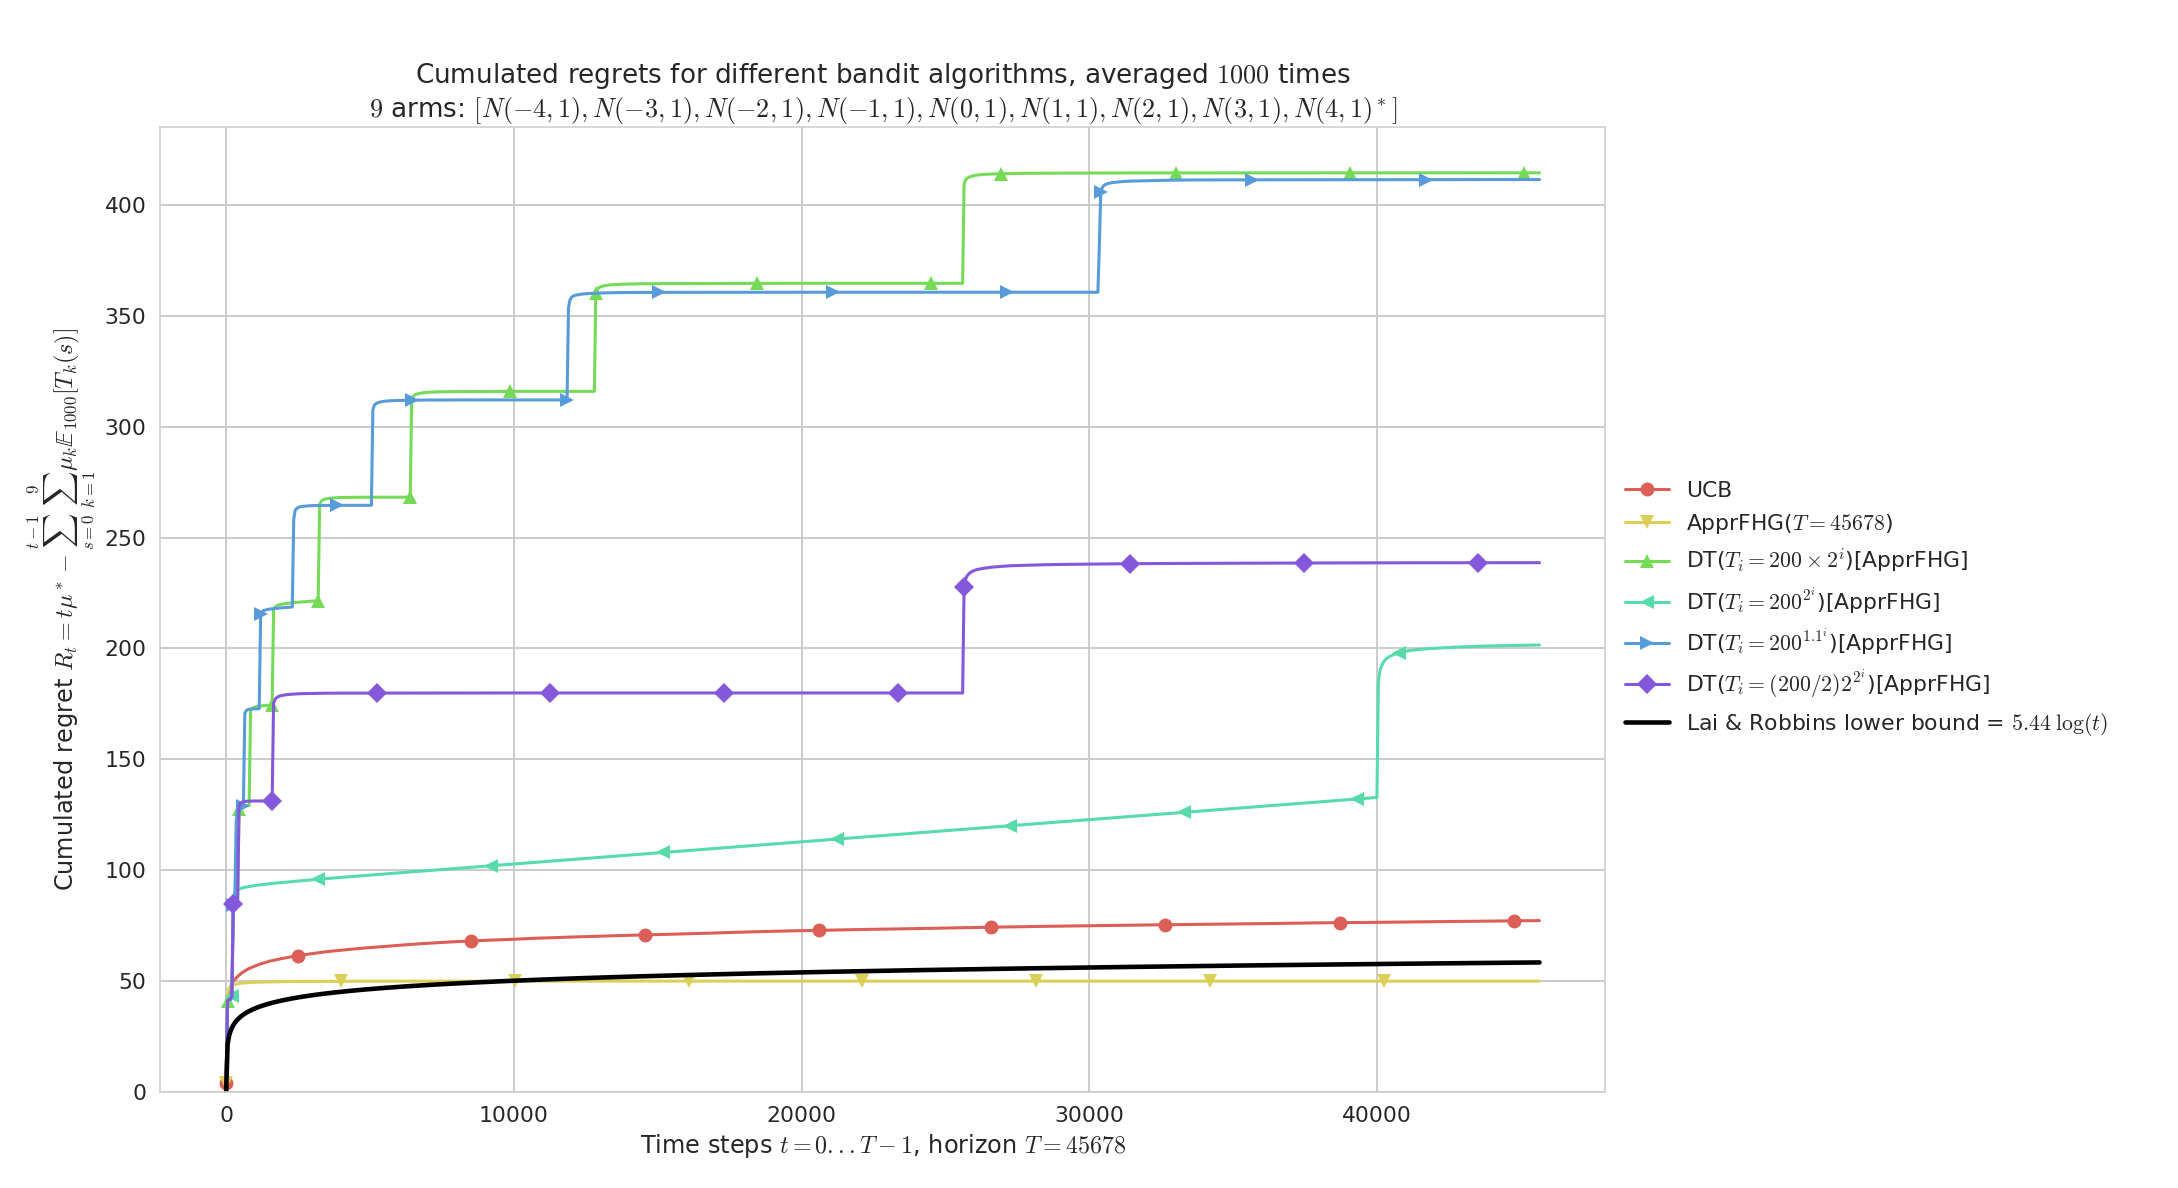
\includegraphics[width=1.00\textwidth]{figures/main____env1-1_6979515539977716717.pdf}
    % \end{subfigure}
    % % ~
    % \begin{subfigure}[!h]{0.49\textwidth}
    %   \includegraphics[width=1.00\textwidth]{XXX.pdf}
    % \end{subfigure}
    \caption{Regret for \DT, for $K=9$ Gaussian arms $\cN(\mu, 1)$, horizon $T=45678$, $n=1000$ repetitions and $\boldsymbol{\mu}$ uniformly spaced in $[-5,5]^K$. On ``easy'' problems like this one, both \UCB{} and \AFHG{} perform similarly and attain near constant regret (identifying the best Gaussian arm is very easy here as they are sufficiently distinct). Each doubling trick also appear to attain near constant regret, but geometric doubling ($b=2$) and slow exponential doubling ($b=1.1$) are slower to converge and thus less efficient.}
    \label{fig:gaussianBandits_DoublingTrick_Restart_fixedProblem2}
    % \vspace*{-15pt}  % XXX remove if problem
\end{figure}

% We include here some experiments on truncated Gaussian Bandits, \ie, bandit problems were each arm has a Gaussian distribution
% % ${\mathcal{N}}_{[a,b]}(\mu, \sigma)$,
% ${\mathcal{N}}(\mu, \sigma)$,
% with known and fixed $\sigma$.
% % and truncated to the interval $[a, b]$.
% In practice, we use
% % $[a, b] = [0, 1]$, $\sigma=0.05$ and $\mu\in[0,1]$.
% $\sigma=1$ and $\mu\in[-5, 5]$.
% %
% We consider a similar setup as the one used for the experiments presented above in Section~\ref{sec:experiments}.

% \FIXME{Copy some figures, include them, talk about it quickly}


\subsection{Experiments with \DTnr}\label{sub:experimentsDTnr}

As mentioned previously, the \DTnr{} algorithm (Algorithm~\ref{algo:DTnr})
is only a heuristic so far, as no theoretical guarantee was proved for it.
%
For the sake of completeness, we also include results from numerical experiments with it, to compare its performance against the ``with restart'' version \DTr.

As expected, \DTnr{} enjoys much better empirical performance,
and in Figs.~\ref{fig:bernoulliBandits_DoublingTrick_noRestart_BayesianProblem} and \ref{fig:bernoulliBandits_DoublingTrick_noRestart_fixedProblem} we see that a geometric or a slow exponential doubling trick with no restart with \KLUCBpp{} can outperform \KLUCB{} and perform similarly to the non-anytime \KLUCBpp.
%
But as observed before, the regret blows up after the beginning of each new sequence if the doubling sequence increase too fast (\eg, exponential doubling).
Despite what is proved theoretically in Theorem~\ref{thm:LowerBoundGeom_log}, here we observe that the geometric doubling is the only one to be slow enough to be efficient.



%
% Regular plots of centralized regrets
%
\begin{figure}[H]
    \centering
    % \begin{subfigure}[H]{0.49\textwidth}
    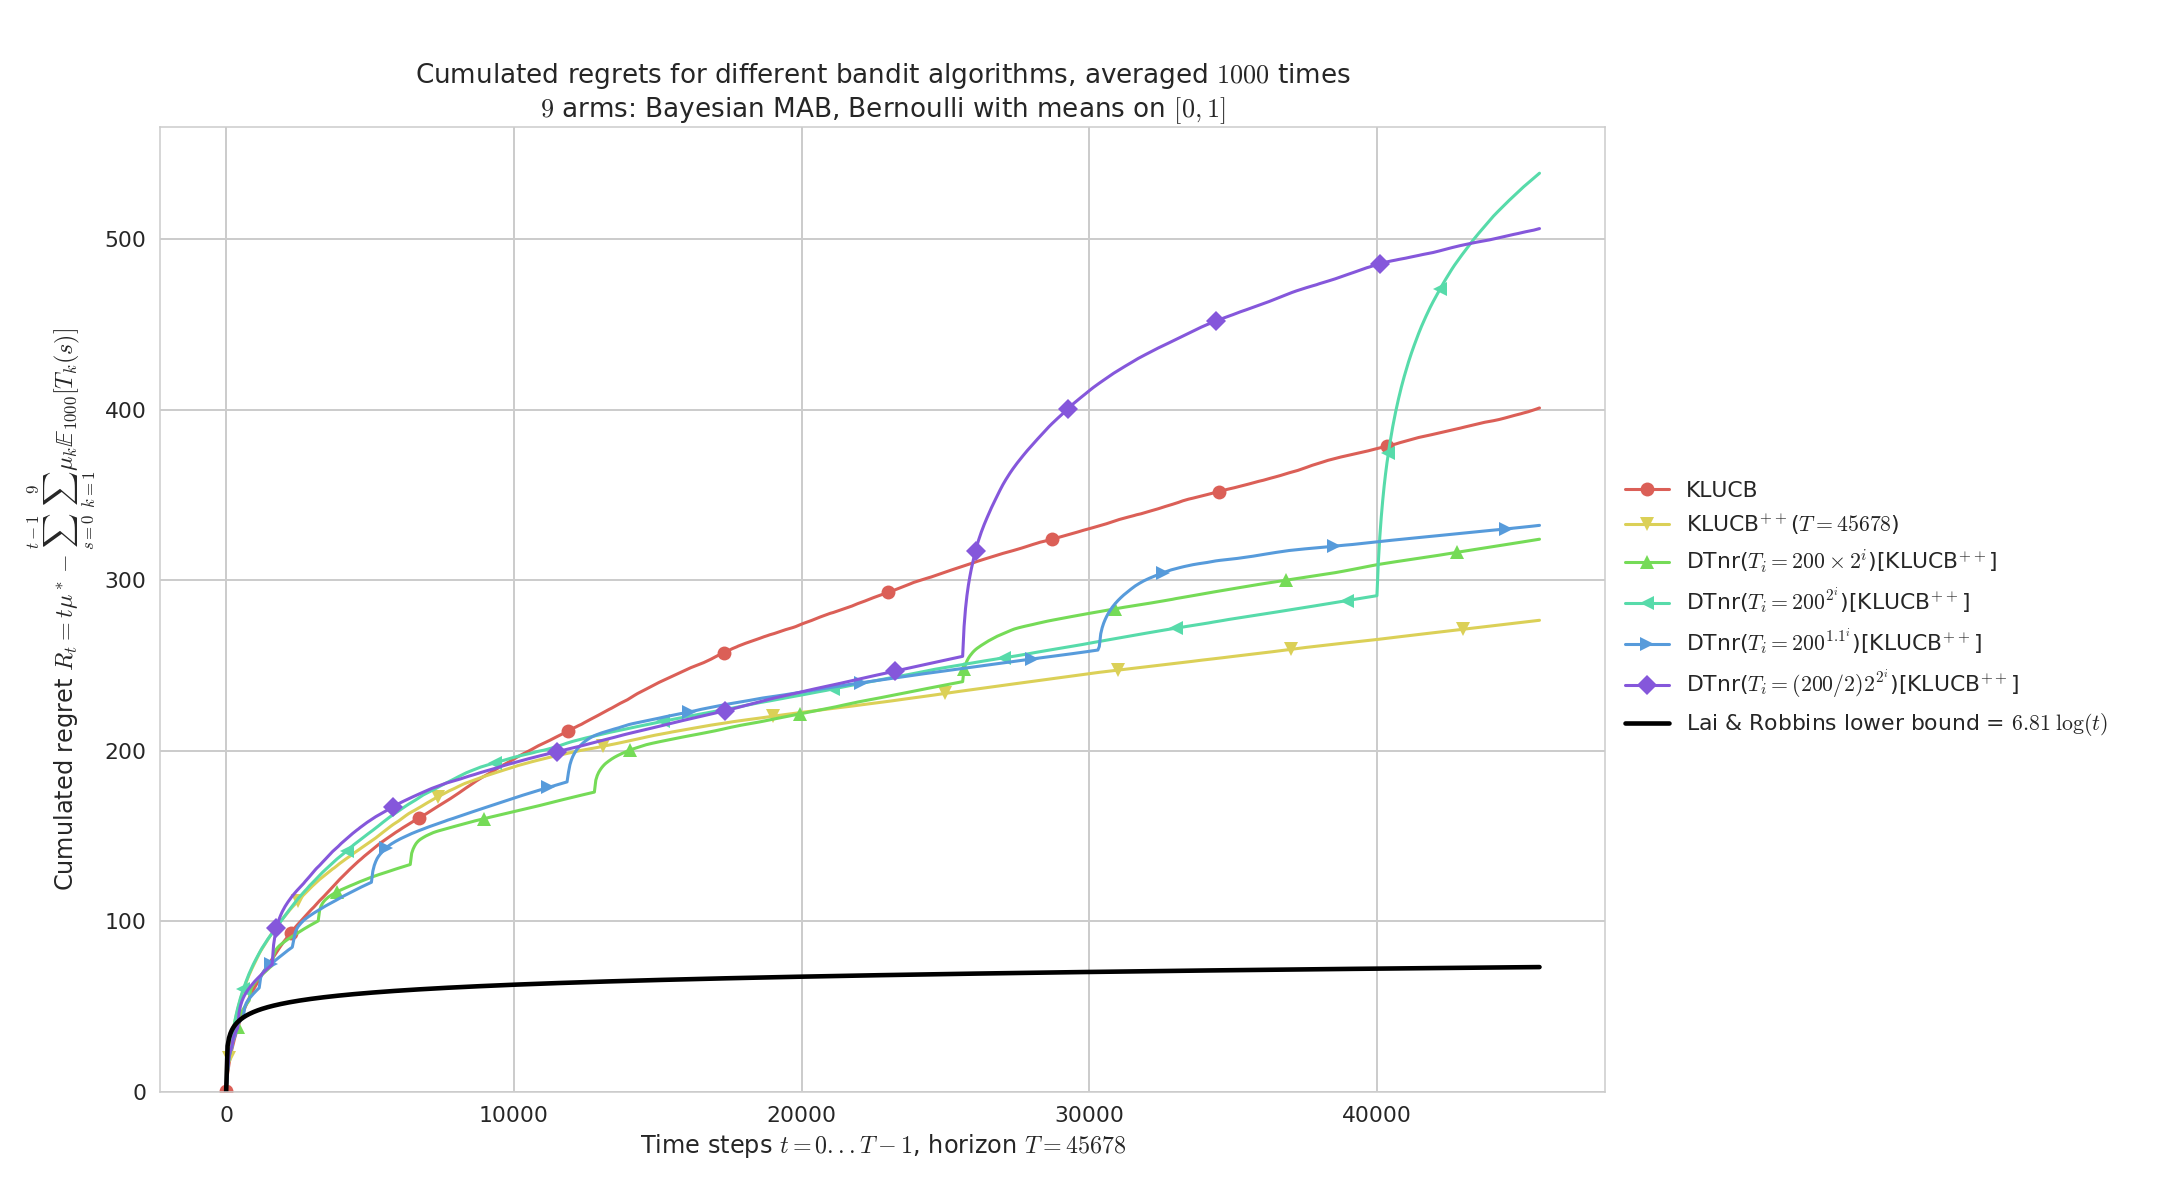
\includegraphics[width=0.92\textwidth]{figures/main____env1-1_5964629015089571121.pdf}
    % \end{subfigure}
    % % ~
    % \begin{subfigure}[H]{0.49\textwidth}
    %   \includegraphics[width=0.92\textwidth]{XXX.pdf}
    % \end{subfigure}
    \caption{Regret for $K=9$ Bernoulli arms, horizon $T=45678$, $n=1000$ repetitions and $\boldsymbol{\mu}$ taken uniformly in $[0,1]^K$, for \DTnr. Geometric doubling (\eg, $b=2$) and slow exponential doubling (\eg, $b=1.1$) are too slow, and short first sequences make the regret blow up in the beginning of the experiment. At $t=40000$ we see clearly the effect of a new sequence for the best doubling trick ($T_i = 200 \times 2^i$). As expected, \KLUCBpp{} outperforms \KLUCB, and if the doubling sequence is growing fast enough then $\DTnr(\KLUCBpp)$ can perform as well as \KLUCB.}
    \label{fig:bernoulliBandits_DoublingTrick_noRestart_BayesianProblem}
    \vspace*{-15pt}  % XXX remove if problem
\end{figure}
%
%
% Regular plots of centralized regrets
%
\begin{figure}[H]
    \centering
    % \begin{subfigure}[H]{0.49\textwidth}
    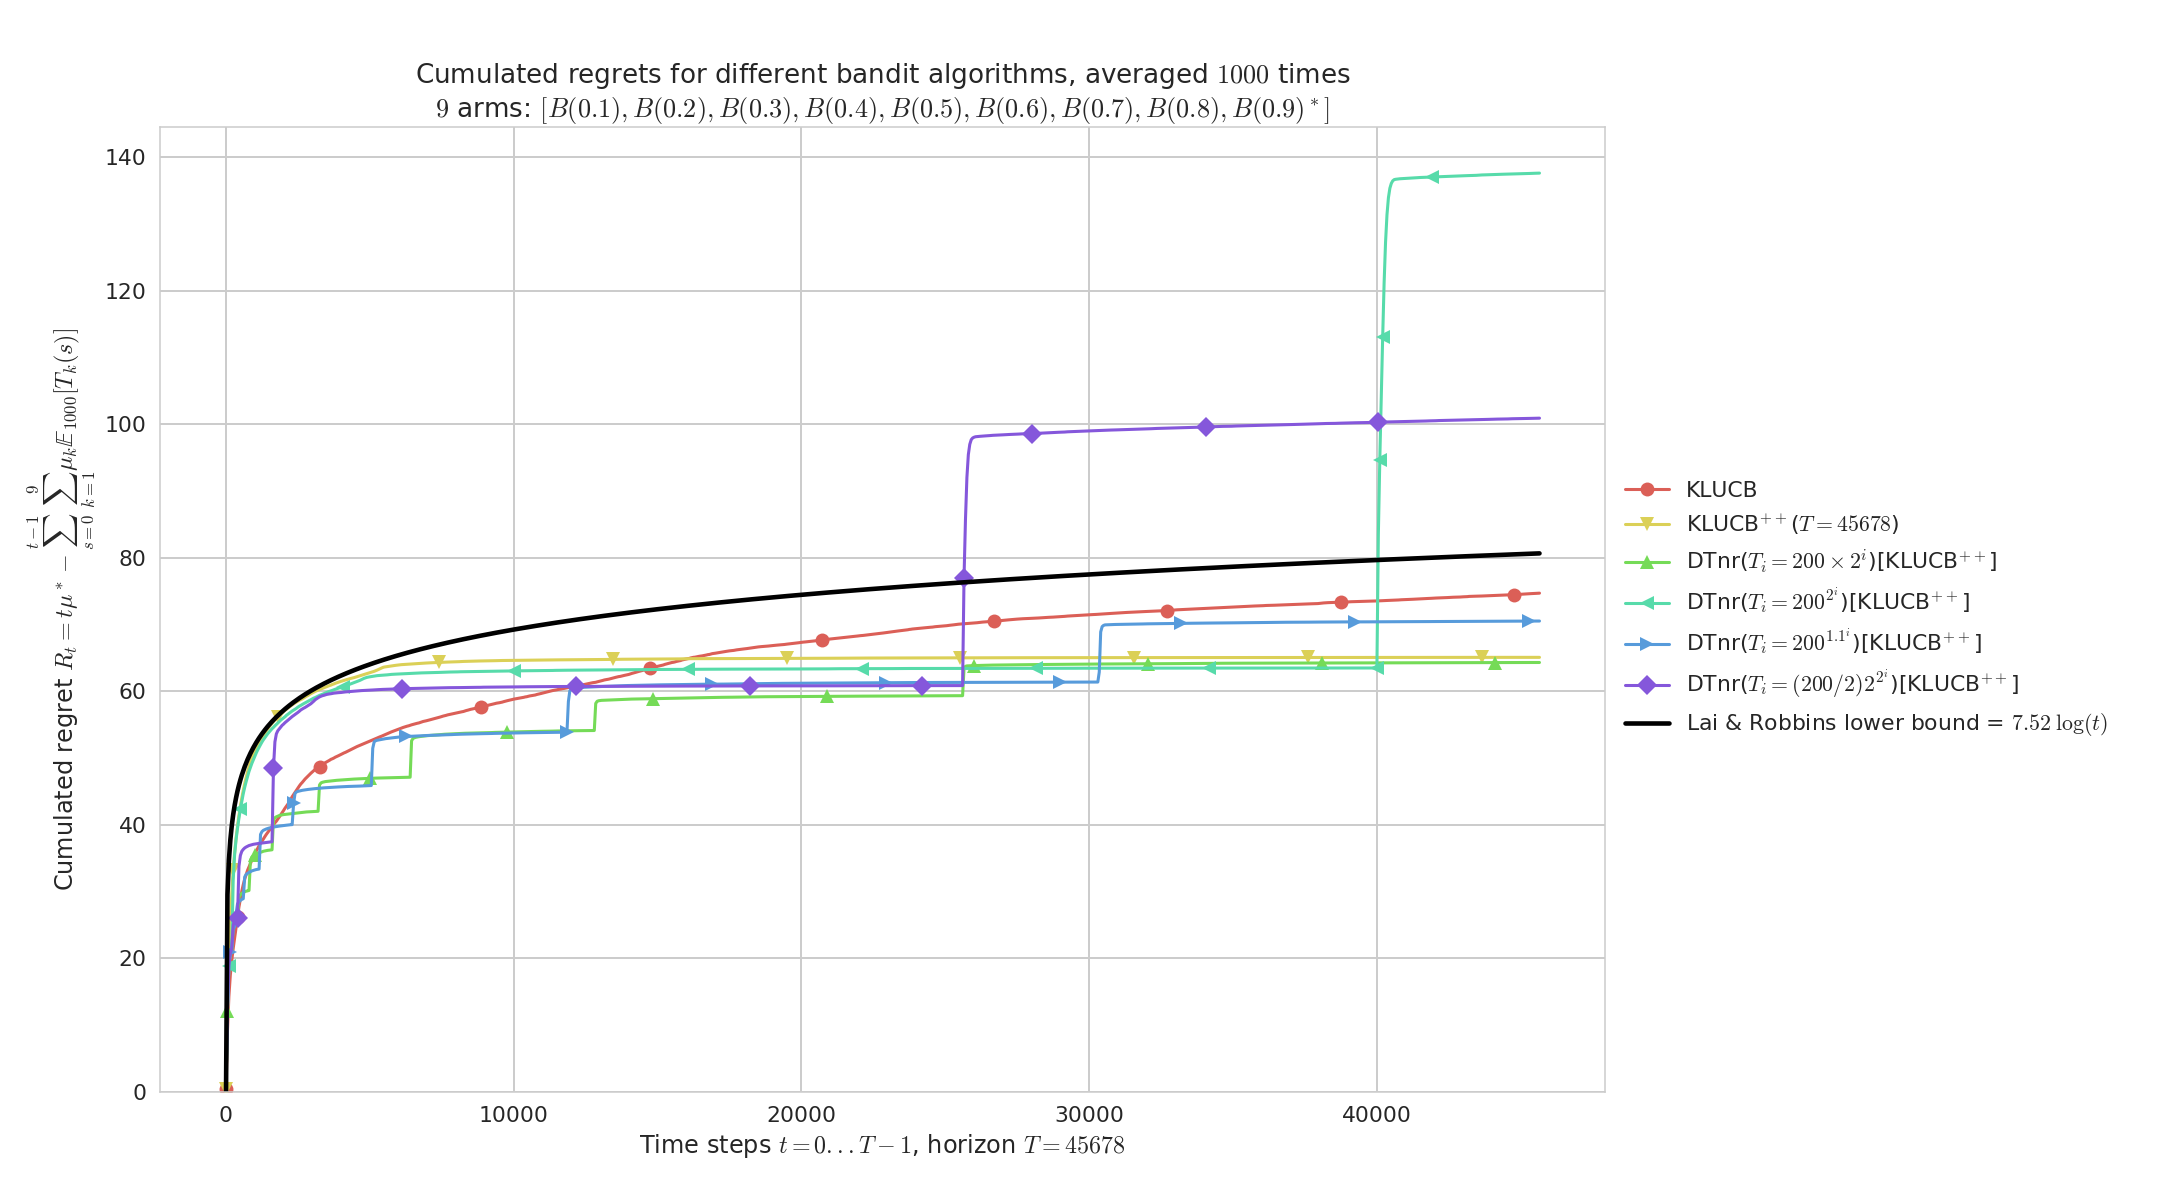
\includegraphics[width=0.92\textwidth]{figures/main____env1-1_5972568793654673752.pdf}
    % \end{subfigure}
    % % ~
    % \begin{subfigure}[H]{0.49\textwidth}
    %   \includegraphics[width=0.92\textwidth]{XXX.pdf}
    % \end{subfigure}
    \caption{$K=9$ Bernoulli arms with $\boldsymbol{\mu}$ evenly spaced in $[0,1]^K$. On easy problems like this one, both \KLUCB{} and \KLUCBpp{} are very efficient, and here the geometric allows the \DTnr{} anytime version of \KLUCBpp{} to outperform both \KLUCB{} and \KLUCBpp.}
    \label{fig:bernoulliBandits_DoublingTrick_noRestart_fixedProblem}
    % \vspace*{-15pt}  % XXX remove if problem
\end{figure}


\hr{}

\section{New Lower Bound in the Intermediate Regime}

\TODO{Lilian: remove all the explanations that are now useless as I extended them in a section above.}
\TODO{Q : for all choices of $f$, do we have that $T_i - T_{i-1}$ (which is increasing) tends to infinity?}

Defining $T_i = \lfloor \exp(\alpha \exp(f(i)))\rfloor$ where $f$ is some increasing function that tends to infinity. The last term operator is
\begin{eqnarray*}
    L_T & = & \min \{ i \in \N : T_{i-1} < T \leq T_i \} \\
    &= & \min \{ i \in \N : f(i) \geq \log\left(\log(T)/\alpha\right)\}.
\end{eqnarray*}
Therefore, it holds that $L_T \geq f^{-1}\left(\log\left(\log(T)/\alpha\right)\right)$.

The usual geometric doubling trick corresponds to $f(i) = \log(i)$, while the exponential doubling trick corresponds to $f$ being a linear function. We provide lower bounds in this section showing that some type of doubling sequence cannot preserve logarithmic bounds.

\begin{theorem}\label{thm:LowerBounds}
    Fix $c$ some constant and let $\cA$ be an online algorithm against a stochastic adversary satisfying
    \[ \forall T \in \N,  R_T(\cA_T) \geq c \; (\log T).\]
    Fix $\alpha \in \R^+$, $b \in (0,1]$ and let $f_b(t) = t^b$. Let $(T_i)_{i\in\N}$ be the doubling sequence associated to $f_b$ and $\alpha$ and denote by $\cA'$ the corresponding doubling algorithm. There exists $\tilde{T}_b$ such that
    \begin{equation}\label{eq:LowerBoundGeom_log_1}
        \forall T \geq \tilde{T}_b, \ \
        R_T(\cA') \geq
        c' \; \left(\log T\right)(\log \log T)^{\frac{1-b}{b}}.
    \end{equation}
\end{theorem}

\TODO{What if we have $\log(T)^{\delta}$ in place of $\log(T)$? the initial common lower bound may not be valid any more}

\TODO{Either fit the $f(t) =\log(t)$ bound in this theorem or state a specific result}

\begin{proof}

We will repeatedly use the fact that for all $x \geq 3$, $\log (x-1) \geq (1/2)\log(x)$. Let $n_1 \in \N^*$ such that for all $i \geq n_1$,
\[\exp\left(\alpha e^{f_b(i)}\right) - \exp\left(\alpha e^{f_b(i-1)}\right) \geq 3 \ \ \text{and} \ \ e^{f_b(i)} - e^{f_b(i-1)} \geq \frac{\log 3}{\alpha}\]
(this is possible as in the two expressions the left hand-side tends to infinity as $i$ tends to infinity).
Note that for all $i\geq 0$,
\begin{eqnarray*}
    T_{i} - T_{i-1} & \geq & \exp\left(\alpha e^{f_b(i)}\right) - \exp\left(\alpha e^{f_b(i-1)}\right) - 1.
\end{eqnarray*}

Using the lower bound \eqref{eq:decompositionIneq_LB} from Lemma~\ref{lem:decomposition} together with the assumption on algorithm $\cA$ yields, for all $T$ such that $L_T \geq n_1 + 1$,
\begin{eqnarray*}
    R_T(\cA') & \geq & c\sum_{i=0}^{L_T-1} (\log(T_i - T_{i-1})) \\
    & \geq & c\sum_{i=0}^{L_T-1} \log\left(\exp\left(\alpha e^{f_b(i)}\right) - \exp\left(\alpha e^{f_b(i-1)}\right) - 1\right)\\
    & \geq & \frac{c}{2}\sum_{i=n_1}^{L_T-1} \log\left(\exp\left(\alpha e^{f_b(i)}\right) - \exp\left(\alpha e^{f_b(i-1)}\right)\right)\\
    & \geq & \frac{c}{2}\sum_{i=n_1}^{L_T-1}\left[\alpha e^{f_b(i-1)} + \log \left(\exp\left(\alpha \left[e^{f_b(i)} - e^{f_b(i-1)}\right]\right) - 1\right)\right] \\
    & \geq & \frac{c}{2}\sum_{i=n_1}^{L_T-1}\left[\alpha e^{f_b(i-1)} + \frac{1}{2} \alpha \left(e^{f_b(i)} - e^{f_b(i-1)}\right)\right] \\
    & = & \frac{c}{2} \left[\sum_{i=n_1}^{L_T-1}\alpha e^{f_b(i-1)} + \frac{1}{2} \alpha \left(e^{f_b(L_T-1)} - e^{f_b(T_1-1)}\right)\right] \\
    & \geq & \frac{\alpha c}{4}\sum_{i=n_1-1}^{L_T-1} e^{f_b(i)} - \frac{c}{4}\alpha e^{f_b(n_1-1)} \\
    & \geq & \frac{\alpha c}{4}\underbrace{\int_{n_1}^{L_T-1} e^{f_b(t)} \dt}_{:=\cI_T} - \frac{c}{4}\alpha e^{f_b(n_1-1)}.
\end{eqnarray*}
In order to prove a lower bound for a specific sequence characterized by $\alpha$ and $f_b$, it is thus sufficient to lower bound the integral $\cI_T$ defined above.

Note that $L_T \geq \left(\log\left(\frac{\log(T)}{\alpha}\right)\right)^{\frac{1}{b}}$ hence
\begin{eqnarray*}
    \cI_T & \geq & \int_{n_1}^{\left(\log\left(\frac{\log(T)}{\alpha}\right)\right)^{\frac{1}{b}} - 1} e^{t^b} \dt =  \frac{1}{b}\int_{n_1^b}^{B_{T,b}}u^{\frac{1-b}{b}}e^u \du,
\end{eqnarray*}
where $B_{T,b}:=\left[\left(\log\left(\frac{\log(T)}{\alpha}\right)\right)^{\frac{1}{b}} - 1\right]^b$, using the change of variable $u = t^b$ (of class $\cC^1$).
Assume now that $T$ large enough so that $B_{T,b} \geq n_1+1$.
Using that $u \mapsto u^{\frac{1-b}{b}}e^u$ is non-decreasing and positive yields
\begin{eqnarray*}
    \cI_T & \geq & \frac{1}{b}\int_{B_{T,b}-1}^{B_{T,b}} u^{\frac{1-b}{b}}e^u \du \geq \frac{1}{b}(B_{T,b} - 1)^{\frac{1-b}{b}}e^{B_{T,b} - 1} \\
    & = & \frac{1}{b e \alpha} (\log T) \left(\log\left({\log T}/{\alpha}\right)\right)^{\frac{1-b}{b}} \times \underbrace{\left(\frac{B_{T,b} - 1}{\log (\log(T)/\alpha)}\right)^{\frac{1-b}{b}}}_{\cE_1(T)} \times \underbrace{e^{B_{T,b}  - \log (\log(T)/\alpha)}}_{\cE_2(T)}.
\end{eqnarray*}

As $B_{T,b} \sim \log (\log(T)/\alpha)$ when $T \rightarrow \infty$, $\cE_1(T) \sim 1$ and there exists some constant $\tilde{T}_1$
such that if $T$ is larger than $T_1$, $\cE_1(T) \geq \frac{1}{2}$.
As for $\cE_2(T)$, it can be rewritten
\[\cE_2(T) = \exp\left(h(\log(\log(T)/\alpha))\right), \ \ \text{with} \ \ h(u) = (u^{1/b} - 1)^b - u.\]

It can be shown that $h(u) \leq 0$ for all $u \geq 1$ and that $h$ is increasing.
Therefore, there exists a constant $c_2 < 0$ such that $h(u) \geq c_2$ for all $u \geq 1$.
Hence, for $T \geq \tilde{T}_2$ such that $\log (\log(T)/\alpha) \geq 1$, $\cE_2(T) \geq \exp(c_2)>0$.
It follows that for $T \geq \tilde{T}_0 = \max(\tilde{T}_1 ,\tilde{T}_2)$,
\begin{eqnarray*}
    \cI_T \geq \frac{e^{c_2}}{2b e \alpha} (\log T) \left(\log\left({\log T}/{\alpha}\right)\right)^{\frac{1-b}{b}}.
\end{eqnarray*}

% for $b=2$ integrating by parts yields
% \begin{eqnarray*}
%  \cI_T & = & 2\int_{\sqrt{T_1}}^{\sqrt{\left(\log\left(\frac{\log(T)}{\alpha}\right)\right)^2 - 1}} ue^{u} \dt\\
%  & = & 2\exp\left(\sqrt{\left(\log\left(\frac{\log(T)}{\alpha}\right)\right)^2 - 1}\right)\left[\sqrt{\left(\log\left(\frac{\log(T)}{\alpha}\right)\right)^2 - 1} -1\right]- 2(\sqrt{T_1} - 1) e^{\sqrt{T_1}}.
% \end{eqnarray*}

\end{proof}


\hr{}

\section{Some thoughts about an upper bound for the exponential doubling}\label{appendix:equivalence_Ti_and_TimTim1}

We study $f(t) = c t$ in this section and study what happens with an algorithm having a $T^{\gamma}$ regret. Note that setting $c=\log (b)$ and $\alpha = \log(a)$ we recovers our previous $T_i  = \lfloor a^{b^i}\rfloor$.

We convinced ourselves in Toulouse that we cannot improve the upper bound with our current technique of upper bounding everything by the last term and evaluating the last term, as this last term $(T_{L_T})^{\gamma}$ can be shown to be ``of order'' to $T^{\gamma e^c}$ (see details below).

One may think that this approach was sub-optimal and study instead the less crude upper bound
\[\sum_{t=0}^{L_T} (T_{i} - T_{i-1})^{\gamma}\]
We start by providing an equivalent of each term in this sum. First note that we will sometimes get rid of some floors when doing asymptotic developments as $\lfloor x_i \rfloor \sim x_i$ for any sequence $x_i \rightarrow \infty$. As $T_i - T_{i-1}  =  T_{i-1}\left(T_i/T_{i-1} - 1 \right) $, we first study
\begin{eqnarray*}
\frac{T_i}{T_{i-1}} & \sim & \exp\left(\alpha (e^{ci} - e^{c(i-1)}\right) = \exp\left(\alpha e^{c(i-1)}(e^c - 1)\right) \\
& = & \left(\exp\left(\alpha e^{c(i-1)}\right)\right)^{e^c -1} \sim (T_{i-1})^{e^c-1}
\end{eqnarray*}
Hence $T_{i}/T_{i-1} - 1 \sim (T_{i-1})^{e^{c}-1}$ and producting two equivalents yields
\[T_{i} - T_{i-1} \sim (T_{i-1})^{e^c} \sim \exp(\alpha e^c \exp(c(i-1)) = \exp(\alpha \exp(ci)) \sim T_i.\]
This actually shows that there is nothing to gain with using the tighter sum (the ``plot'' should thus have been increasing...)

More precisely, our analysis is tight in the following sense

\begin{lemma} For any exponential doubling sequence,
\[\sum_{i=0}^{n}T_i^{\gamma} \underset{n \rightarrow \infty}{=} \Theta(T_n^{\gamma})\]
\end{lemma}

\TODO{E: I am pretty sure we proved that in Toulouse}

If this is true, then I can prove the following:
\[\limsup_{T\rightarrow \infty} \frac{\log\left[\sum_{i=0}^{L_T} (T_i - T_{i-1})^{\gamma}\right]}{\log [T^{\gamma}]} = e^c\]
and
\[\liminf_{T \rightarrow \infty} \frac{\log\left[\sum_{i=0}^{L_{T}-1} (T_i - T_{i-1})^{\gamma}\right]}{\log [T^{\gamma}]} = e^{-c}\]
which shows that we cannot hope for better than our previous upper and lower bounds if we start from the Lemma~\ref{lem:decomposition}. And as for a non-anytime algorithm, we can never control the intermediate regret $R_t$ for $t\leq T$, we have not hope to be able to use what happens between $L_{T} - 1$ and $L_T$ hence Lemma~\ref{lem:decomposition} was not such a bad start...

\TODO{E: if needeed, I will imput the proof}

Maybe we need something slightly slower, like $f(i) = ci/\log(i)$, I will try to check numerically whether $T_{L_T} = \Theta(T)$ in that case (which is what would make the upper bound work...)

\end{document}
